\documentclass[a4paper, 12pt]{report}

\usepackage[left = 3cm, top = 2.5cm, bottom = 1.5cm, right = 2cm]{geometry}
\usepackage{graphicx}
\usepackage[spanish,es-tabla]{babel} % Idioma español con tablas
\usepackage{amsmath}
\usepackage{amssymb}
\usepackage{amsfonts}
\usepackage[utf8]{inputenc}         % Para escribir en castellano
\usepackage[T1]{fontenc}
\usepackage{color}
\usepackage{alltt}
\usepackage{times}
\usepackage{latexsym}
\usepackage{anyfontsize}
\setcounter{secnumdepth}{3} %para que ponga 1.1.1.1 en subsubsecciones
\setcounter{tocdepth}{3}    % para que ponga subsubsecciones en el indice
\usepackage{setspace}       % Usado para %\onehalfspace  \doublespacing  \singlespace
\usepackage{booktabs}       % Para formar tablas
%\usepackage{longtable}     % Usado para diseñar grandes tablas.

%\usepackage{algorithmic}
%\usepackage{algorithm}


\usepackage{changepage}
\newenvironment{h1}[2][]{\section[#1]{#2}}{}
\newenvironment{h2}[2][]{%
  \begin{adjustwidth}{2em}{}
    \subsection[#1]{#2}%
}{%
  \end{adjustwidth}
}
\newenvironment{h3}[2][]{%
  \begin{adjustwidth}{2em}{}
    \subsubsection[#1]{#2}%
}{%
  \end{adjustwidth}
}



%%%%==nuevos==========%%%%
\usepackage[normalem]{ulem} %%agregado por ul
\useunder{\uline}{\ul}{} %%agregado por ul
\usepackage{float} %% agregado para reconocer H
\usepackage{url}
\usepackage[font=small,skip=0pt]{caption}
\captionsetup{justification=centering,margin=1cm}

\usepackage{parskip}
\setlength{\parindent}{15pt}
%%%%==nuevos==========%%%%

%%%%%%%%%%%%%%%%%%%%%%%%%%%%%%%
%%% Tables-related packages %%%
%%%%%%%%%%%%%%%%%%%%%%%%%%%%%%%
\usepackage{multirow}
\usepackage{multicol}
\usepackage{array,colortbl}

\usepackage[round]{natbib}

\newcommand{\yy}{{\'{\i} }}
\newcommand{\y}{\'{\i}}
\usepackage{xcolor} %para color

\usepackage{lscape} %para landscape pages # 		\being & \end {landscape}

\begin{document}

\baselineskip 1cm
\pagestyle{plain}
	%!TEX root = origin.TEX
%%%%%%%%%%%%%%%%%%%%%%%%%%%%% CARATULA%%%%%%%%%%%%%%%%%%%%%%%
  \textheight 19cm
  \pagestyle{empty}
  \begin{center}
   {\bf {\fontsize{14}{16.8}\selectfont UNIVERSIDAD NACIONAL DE TRUJILLO}}     
   
      {\bf{\fontsize{14}{16.8}\selectfont Facultad de Ciencias Físicas y Matemáticas}} 

    {\bf{\fontsize{14}{16.8}\selectfont Escuela Profesional de Informática}}
  \end{center}  

  \begin{figure}[ht]
  \begin{center}
  
\includegraphics[width=.4\textwidth]{images/unt}
  \end{center}
  \end{figure}

  \vskip 1.15cm
  \begin{center}
    {  
      {\bf \fontsize{17}{20.4}\selectfont{MODELO DE RECONOCIMIENTO AUTOMÁTICO DE SEÑALES DE TRÁNSITO VEHICULAR MEDIANTE APRENDIZAJE PROFUNDO DE REDES NEURONALES CONVOLUCIONALES }}     
      \vskip 3cm
      {\bf \fontsize{14}{16.8}\selectfont {\hspace{-0.4cm}AUTOR: Josué Gastón Távara Idrogo}}\\
      \vskip 0.2cm
      {\bf \fontsize{14}{20.4}\selectfont{\hspace*{-1.7cm} ASESOR: Jorge Luis Gutierrez Gutierrez }}  
    } 
  \end{center}   

  \vskip 1.1cm
  \begin{center}    
  {\bf {\fontsize{14}{16.8}\selectfont Trujillo - Perú
  \vskip 0.0cm
  \hspace*{-0.2cm} 
  2019 }}
  \end{center} 
  \newpage


%%%%%%%%%%%%%%%%%%%%%%%%%%%%CONTRA CARATULA 1 %%%%%%%%%%%%%%%%%%%%%%%%%%%%%
  \newpage
  \pagestyle{plain}
  \pagenumbering{roman}

  \hspace*{6cm}
  \vskip 9cm
  \begin{center}
     {\bf \doublespacing {\fontsize{17}{20.4}\selectfont{MODELO DE RECONOCIMIENTO AUTOMÁTICO DE SEÑALES DE TRÁNSITO VEHICULAR MEDIANTE APRENDIZAJE PROFUNDO DE REDES NEURONALES CONVOLUCIONALES }}}     
  \end{center} 
  \newpage


%%%%%%%%%%%%%%%%%%%%%%%%%%%%% CONTRA CARATULA 2 %%%%%%%%%%%%%%%%%%%%%%%
  \begin{center}
   {\bf {\fontsize{14}{16.8}\selectfont{JOSUÉ GASTÓN TÁVARA IDROGO}}}
   \end{center}   

  \vskip 3.2cm

  \begin{center}
     {\bf \doublespacing {\fontsize{17}{20.4}\selectfont{MODELO DE RECONOCIMIENTO AUTOMÁTICO DE SEÑALES DE TRÁNSITO VEHICULAR MEDIANTE APRENDIZAJE PROFUNDO DE REDES NEURONALES CONVOLUCIONALES }}}     
  \end{center}   
    \vskip 2cm
  \begin{verse}
   \fontsize{12}{14.4}\selectfont{\hspace*{0.6cm}Tesis presentada a la Escuela Profesional de Informática en la Facultad de Ciencias Físicas y Matemáticas de la Universidad Nacional de Trujillo, como requisito para la obtención del Título profesional de Ing. Informático}
  \end{verse}

  \vskip 1.5cm 
  {\fontsize{14}{16.8}\selectfont ASESOR: DR. JORGE LUIS GUTIERREZ GUTIERREZ} 
  \vskip 1cm 
  
  \begin{center}    
  \vskip 1.8cm
  {
  \fontsize{14}{16.8}\selectfont Trujillo - Perú
  \vskip 0.2cm  \hspace*{-0.2cm} 2019
  }
  \end{center} 
  \newpage


%%%%%%%%%%%%%%%%%%%%%%%%%%%%HOJA DE APROBACION %%%%%%%%%%%%%%%%%%%%%%%%%%%%%
\begin{center}
 {\bf {\Large HOJA DE APROBACIÓN }     
 \vskip 1.5cm
  {\Large Modelo De Reconocimiento Automático De Señales De Tránsito Vehicular Mediante Aprendizaje Profundo De Redes Neuronales Convolucionales }}
 \vskip 1cm 
  {\large{Josué Gastón Távara Idrogo}}\\

 \vskip 1cm
\end{center} 
Tesis defendida y aprobada por el jurado examinador:
\vskip 1.2 cm
\begin{flushleft} 
$\overline{\mbox{Prof. Dr. Jorge Luis Gutierrez Gutierrez - Asesor}}$\\
\vskip -0.5cm
Departamento de Informática - UNT
\end{flushleft} 
\vskip 1cm
\begin{flushleft} 
$\overline{\mbox{Prof. Mg. Anthony Gomez Gonzales}}$\\
\vskip -0.5cm
Departamento de Informática - UNT
\end{flushleft} 
\vskip 1cm
\begin{flushleft} 
$\overline{\mbox{Prof. Mg. Jose Luis Peralta Luján}}$\\
\vskip -0.5cm
Departamento de Informática - UNT
\end{flushleft}
\vskip 0.5cm 
\begin{center}    
Trujillo, DIA de MES del 2019
\end{center} 
\newpage
%%%%%%%%%%%%%%%%%%%%%%%%%%%%%%%%%%%%%%%%%%%%%%%%%%%%%%%%%%%%%%%%%%%%%%%%%%%%


%%%%%%%%%%%%%%%%%%%%%%%%%%%% DEDICATORIA %%%%%%%%%%%%%%%%%%%%%%
 
 \addcontentsline{toc}{chapter}{Dedicatoria}
 {\bf\Large {Dedico esta tesis a :}}
 \vskip 1cm
  \begin{quotation}
  {\it Mi madre María y mi padre Gastón; amare et sapere vix deo concesitur.
    \vskip 1cm
    Mis hemanas Carol y Marita por el apoyo continuo.
  }
 \end{quotation}


%%%%%%%%%%%%%%%%%%%%%%%%%%%% AGRADECIMENTOS %%%%%%%%%%%%%%%%%%%%%%
  \newpage
  \addcontentsline{toc}{chapter}{Agradecimientos}
  {\bf\Large {\flushleft{Agradecimientos}}}
  \vskip 1.5cm
  \begin{quotation}
  Agradezco a Dios por haberme bendecido en toda mi vida.
  \vskip 1cm
  A mis profesores del Departamento de Informática, de los cuales recibí una gran cantidad de conocimientos y apoyo que formaron parte fundamental en el desarollo de mi carrera universitaria.
  \vskip 1cm
  A mi asesor Dr. Jorge Luis Gutierrez Gutierrez de la Universidad Nacional de Trujillo, que siempre se mostró disponible, interesado y capacitado para ayudarme, otorgándome las sugerencias necesarias para redactar esta investigación.
  \vskip 1cm
  A la profesora Dra. Roseli Aparecida Francelin Romero de la Universidad de Sao Paulo por haber introducido el tema de Deep Learning en mi instancia como estudiante de esa universidad y haberme sugerido temas de investigación en esta área.

  \vskip 1cm
  \end{quotation}


%%%%%%%%%%%%%%%%%%%%%%%%%%%% RESUMEN%%%%%%%%%%%%%%%%%%%%%%
  \newpage
  \begin{center}
   \addcontentsline{toc}{chapter}{Resumen}
   {\bf\LARGE Resumen}
  \end{center} 
  \vskip 0.5cm
  \begin{quotation}
  
  La presente investigación tiene por objetivo principal implementar un modelo basado en el aprendizaje profundo de redes neuronales convolucionales para reconocer automáticamente señales de tránsito vehicular usando fundamentos de cálculo matemático, técnicas de procesamiento de imágenes y algoritmos de inteligencia artificial.
  \vskip 0.2cm
  El proyecto se centra en un grupo de señales de Tránsito vehicular de Alemania y Perú, identificando 43 y 7 categorías respectivamente. Iniciando con  la adquisición de imágenes, se procedió realizar el procesamiento de estas con la finalidad de aumentar el conjunto de datos y poder ejecutar el aprendizaje profundo a través de diversos diseños de arquitecturas de redes neuronales convolucionales.
  \vskip 0.2cm
  Como resultado final, se obtuvo un modelo con buenos indicadores y resultados en el reconocimiento de señales de tránsito vehicular. De esta manera, se pretende contribuir en los esfuerzos de la industria automotriz en el campo de sistemas avanzados de asistencia al conductor así como también puede formar parte de diversos mecanismos que buscan dar soluciones a la inseguridad vial.

  \vskip 0.2cm
  {\bf Palabras claves:} aprendizaje profundo, redes neuronales convolucionales, procesamiento de imágenes.
  \end{quotation}


%%%%%%%%%%%%%%%%%%%%%%%%%%%%ABSTRACT%%%%%%%%%%%%%%%%%%%%%%
  \newpage
  \begin{center}
   \addcontentsline{toc}{chapter}{Abstract}
   {\bf\LARGE Abstract}\vskip 1.5cm
  \end{center} 
  \begin{quotation}

  The main objective of this research is to implement a model based on the deep learning through convolutional neural networks to automatically recognize vehicular traffic signals using mathematical calculation funds, image processing techniques and artificial intelligence algorithms.
  \vskip 0.2cm
  
  The project focuses on a group of traffic signals from Germany and Peru, identifying 43 and 7 categories respectively. Starting with the acquisition of images, the processing of these activities is carried out with the purpose of increasing the data set so then be able to carry out in-depth learning through various designs of convolutional neural network architectures.
  \vskip 0.2cm

  As a final result, a model with good indicators and results in the recognition of vehicular traffic signals was obtained. In this way, it is intended to contribute to the efforts of the automotive industry in the field of Advanced driver-assistance systems(ADAS), as well as being part of various mechanisms that seek to provide solutions to road safety.
  \vskip 0.3cm
  \hspace*{-0.6cm}{\bf Keywords:} deep learning, convolutional neural networks, image processing.
  \end {quotation}



%%%%%%%%%%%%%%%%%%%%%%%%%%% LISTA DE SIMBOLOS %%%%%%%%%%%%%%%%%%%%%%
%\newpage
%\addcontentsline{toc}{chapter}{Lista de símbolos}
% {\bf\LARGE Lista de símbolos(FALTA POR PRECISAR)}
% \vskip 1.5cm
%Constantes: 
%\begin{enumerate}
%\item[(1)]$\otimes$ \hspace*{0.8cm}Simbolo de convolución}
%\item[(2)] $n $ \hspace*{1.1cm} Indice de bienes finales deseados por los consumidores.
%\item[(3)] ...
%%\vskip 3cm
%\end{enumerate} 
%%\vskip 0.3cm
%Variables:
%\begin{enumerate}
%\item[(5)] $ x^{r} $ \hspace*{1cm} Vector columna que denota la actividad de producción.
%\item[(6)] $ u^{r} $ \hspace*{1.2cm} . . .
%\end{enumerate}
    % caratula del trabajo
\listoffigures      % indice de figuras
\addcontentsline{toc}{chapter}{Índice de Figuras}
\listoftables       % indice de tablas
\addcontentsline{toc}{chapter}{Índice de Tablas}
\textheight 24cm 	% footer height
\tableofcontents    % indice de materias
	%!TEX root = origin.TEX
\chapter{Introducción}
	\pagenumbering{arabic}
	\setcounter{page}{1}
	\renewcommand{\baselinestretch}{1} %doble espacio paratodo el texto
	Al conducir en carreteras congestionadas, a veces es difícil mantener los ojos en todas partes a la vez, comprobando el camino por delante, el tráfico venidero, lo que está detrás de usted, tratar de mantener su velocidad; es por ello, que existen mecanismos destinados a reglamentar el tránsito, advertir o informar a los usuarios mediante palabras, sonidos o símbolos determinados. Un claro ejemplo de ello, es la policía de tránsito o las señalizaciones vehiculares que según sea el caso, en todos los países regulan el tránsito e informan al usuario sobre direcciones, rutas, destinos, así como dificultades existentes en las carreteras y previenen cualquier peligro que podría presentarse en la circulación vehicular.

	\vskip 0.15cm
	Sin embargo, cuando estos mecanismos no son conocidos o percibidos pueden ocasionar no solo que la congestión del tráfico aumente, sino que también se produzcan accidentes que en muchos casos derivan en consecuencias fatales, generando inseguridad vial.

	\vskip 0.15cm
	La inseguridad vial es un problema de interés mundial, según el último informe de la OMS (Organización Mundial de la salud) anualmente cerca de 1,3 millones de personas mueren alrededor del mundo y entre 20 y 50 millones padecen traumatismos no mortales \citep{OMS}. Esto representa la segunda de las principales causas de muerte a nivel mundial entre los jóvenes de 5 a 29 años de edad, y la tercera entre la población de 30 a 44 años. Son distintas las causas que conllevan a este problema, de las cuales las principales pueden ser la falta de concientización y educación vial. 
	
	\vskip 0.15cm	
	Es un problema para la economía mundial de los países, así también para los hogares. A pesar de ello, se invierte muy poco dinero en prevenir los accidentes y las lesiones causadas por el tránsito. El sector salud se beneficiaría mucho de una mejor prevención de las lesiones porque se reducirían las hospitalizaciones y la gravedad de los traumatismos \citep{CNSV}.

	\vskip 0.15cm
	Los usuarios vulnerables de la vía pública representan la mitad de todas las muertes por accidente de tránsito a nivel mundial y es mayor en países de ingresos bajos, siendo la causa principal, el aumento de velocidad durante la conducción de los vehículos \citep{OMS}.

	\vskip 0.15cm
	\begin{figure}[H]
	\begin{center}
	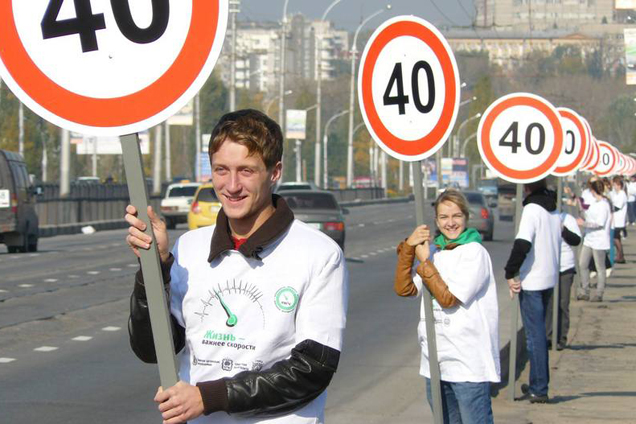
\includegraphics[width=0.5\textwidth]{images/intro/velocidad}
	\end{center}
	\begin{center}
	\caption{\small{Señalización de velocidad}}
	{\small{Fuente: \cite{OMS}}}
	\end{center}
	\vspace{-1.5em}
	\end{figure}
	
	Por otra parte, de los vehículos que se venden en el 80\% de los países no cumplen las normas básicas de seguridad, es por ello que se debe trabajar en obtener vehículos más seguros ya que es un factor fundamental para prevenir de alguna forma los accidentes de tránsito o reducir la probabilidad de traumatismos graves en caso de que estos se produzcan \citep{OMS}.
	
	\vskip 0.15cm
	En lo que respecta al sector nacional, es decir en el Perú, la inseguridad vial es un problema constante ya que los peruanos mueren más por los accidentes de tránsito que por la inseguridad ciudadana según datos mostrados por María Edith Baca de la Organización Panamericana de la Salud \citep{OPS}. Adicionalmente, según un estudio realizado por RPPData en base a reportes de la Policía publicados entre el 2010 y el 2016, en el país cada día fallecen 8 personas en accidentes de tránsito, \citep{RPPData}. El costo de estas muertes, calculado en S/ 19,165 millones por la consultora Alauda especializada en mantenimiento de infraestructura, representó un 3.1\% del PBI \citep{Gestion2}.  
	
	
	\vskip 0.15cm
	En el 2016 se obtuvo un índice Global de Satisfacción del Conductor \citep{CNN} en el cual, Perú y la capital Lima se encuentran respectivamente en la lista de peores países y ciudades para conducir en América Latina, esto se ve reflejado en que los últimos años se ha incrementado el índice de mortandad originados por los accidentes de tránsito siendo las principales causas de los mismos el exceso de velocidad, estado de ebriedad del conductor, imprudencia temeraria y el desacato a las señales de tránsito, todas ellas de responsabilidad directa del conductor del vehículo motorizado al no respetar las señales de tránsito\citep{SUTRAN}. 
	
	\begin{figure}[H]
	\begin{center}
	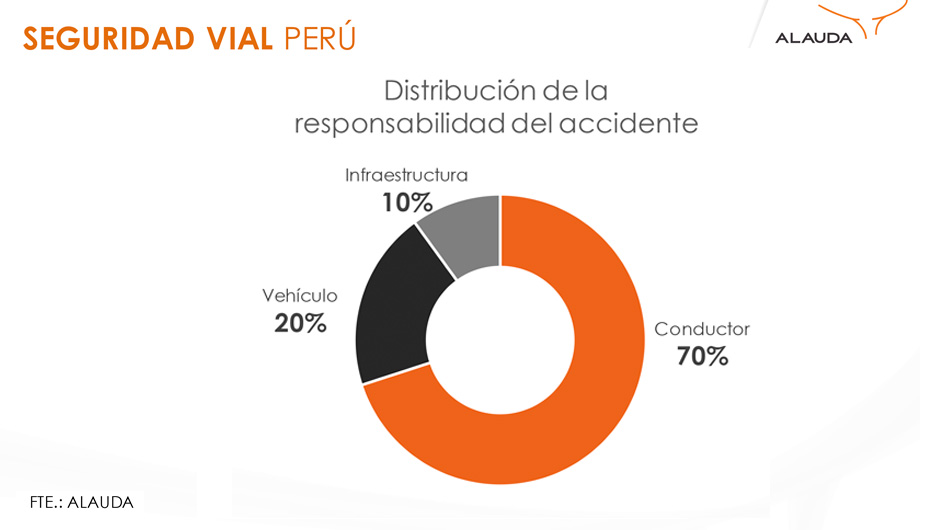
\includegraphics[width=0.5\textwidth]{images/intro/responsabilidad_cond}
	\end{center}
	\begin{center}
	\caption{\small{Análisis de responsabilidad de accidentes}}
	{\small{Fuente acceso: \cite{Gestion1}}}
	\end{center}
	\vspace{-1.5em}
	\end{figure}

	\begin{figure}[H]
	\begin{center}
	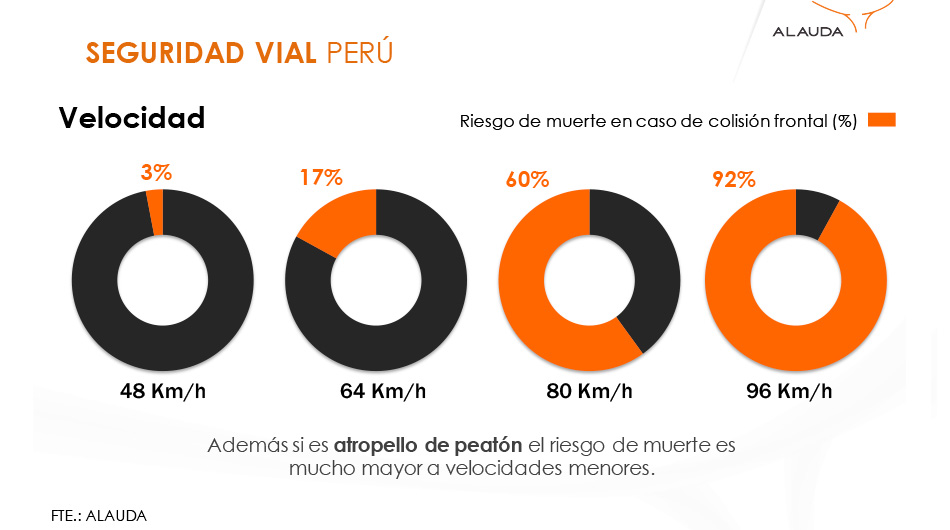
\includegraphics[width=0.6\textwidth]{images/intro/velocidad_ind}
	\end{center}
	\begin{center}
	\caption{\small{Influencia de velocidad en accidentes}}
	{\small{Fuente acceso: \cite{Gestion1}}}
	\end{center}
	\vspace{-1.5em}
	\end{figure}
	
	%Aunque se han publicado algunos estudios sobre este tema, aún no existen comparaciones sistemáticas de enfoques que sean imparciales y no se dispone de conjuntos de datos de referencia completos. 
	
	El reconocimiento de estas señales es un problema de clasificación multi-categórica que comúnmente presenta desigualdades en las frecuencias de aparición de sus clases. Además, las señales de tránsito muestran una amplia gama de variaciones entre las clases en términos de color, forma y la presencia de símbolos, leyendas o texto. Además, existen subconjuntos de clases (por ejemplo, signos de límite de velocidad) que son muy similares entre sí, lo que representa un reto para un reconocedor  automático, el cual tiene que hacer frente a grandes variaciones en las apariencias visuales debido a cambios de iluminación, oclusiones parciales, rotaciones, condiciones meteorológicas, escalamiento, etc.
    

	
\section{Justificación de la investigación} 

	\subsection{Justificación Académica}

	Recientemente las redes convolucionales profundas han superado los métodos tradicionales de aprendizaje en la clasificación de imágenes. Con los rápidos avances de las estructuras de algoritmos de aprendizaje profundo y la factibilidad de su implementación de alto rendimiento con unidades de procesamiento gráfico (GPU), es ventajoso investigar en problemas de clasificación de imágenes desde la perspectiva de un aprendizaje profundo eficiente. Sin embargo, realizar esto no es tarea simple, ya que se requiere de un modelo de reconocimiento que funcione para imágenes que se encuentran comúnmente influenciadas por la iluminación, la orientación, la variación de velocidad de los vehículos, entre muchos otros problemas más.  \vskip 0.2cm

	En este sentido, esta investigación pretende la elaboración de un modelo basado en el aprendizaje profundo de redes convolucionales que permita el reconocimiento de señales de tránsito vehicular. La siguiente figura muestra un diagrama de bloques con la secuencia de actividades que demanda el reconocimiento.

	\begin{figure}[H]
	\begin{center}
	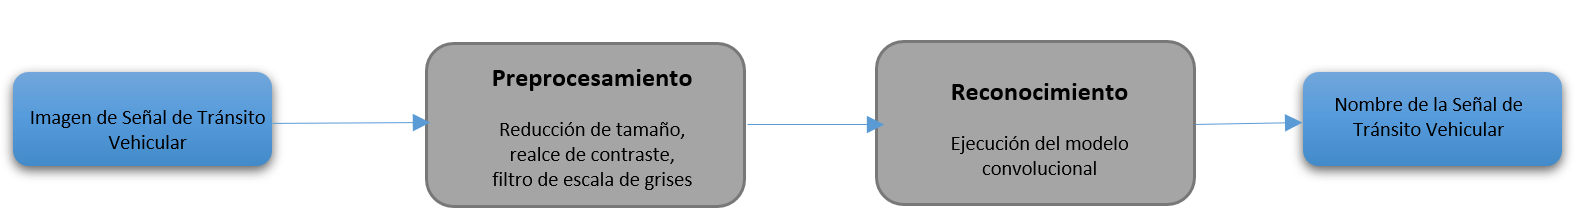
\includegraphics[width=0.8\textwidth]{images/intro/bloque}
	\end{center}
	\begin{center}
	\caption{\small{Diagrama de bloques para el reconocimiento}}
	{\small{Fuente: Elaboración propia}}
	\end{center}
	\vspace{-1.5em}
	\end{figure}


	Por lo tanto, la importancia de esta investigación en el punto de vista de ciencias de la computación se justifica en poner en práctica los conocimientos adquiridos en la formación académica, siendo los más resaltables el tema de procesamiento de imágenes e inteligencia artificial con la finalidad de obtener un modelo robusto de redes neuronales convolucionales basadas en el aprendizaje profundo (deep learning) que permita analizar el contenido de imágenes para el reconocimiento de señales de tránsito vehicular. 


	\subsection{Justificación Social}
	
	Teniendo conocimiento de lo descrito al inicio de este capítulo, la visibilidad y conocimiento de señales de tráfico es crucial para la seguridad de los conductores y es por ello que la introducción de un modelo de reconocimiento de señales de tránsito que funcione en diferentes contextos puede formar parte de la solución a que se puedan evitar constantes infracciones y muertes, y en consecuencia reducir estos índices progresivamente. Por ejemplo, el reconocimiento de estas señales en el momento de la conducción puede ofrecer la posibilidad de dar una notificación al no darse cuenta de un cambio en el límite de velocidad, el aviso de que se está cometiendo una infracción al girar o estacionarse donde no se debe o la advertencia de un peligro potencial por delante. Por otro lado, cuando usuarios desconocen de alguna señal de tránsito, una aplicación móvil que dé la posibilidad de reconocer automáticamente aquella señal serviría como aporte en la educación vial.\vskip 0.2cm

	Por lo tanto, esta investigación es importante porque a través de un modelo que reconozca señales de tránsito vehicular se podría contribuir en la industria automotriz, específicamente en los sistemas avanzados de asistencia al conductor (del inglés, \textit{ADAS}); así como también se ha descrito anteriormente, el modelo pretendido puede ser usado en diferentes plataformas y formar parte de diversos mecanismos que buscan dar soluciones a la inseguridad vial. \vskip 0.2cm
	
	Todos los hechos descritos hacen que el reconocimiento de las señales de tránsito sea un reto desafiante y esencial en muchos aspectos, no solo para contribuir en los esfuerzos de la industria automotriz en el campo de la asistencia al conductor, sino también incluso para organismos gubernamentales quienes se dan cuenta de la problemática que representa la inseguridad vial y buscan constantemente introducir nuevos mecanismos y tecnologías que faciliten y mejoren la conducción vehicular para el beneficio propio del conductor y en general para la seguridad vial en la sociedad.


\section{Formulación del problema}

  En este trabajo, se propone discutir el modelo de redes neuronales convolucionales basado en el problema del reconocimiento de imágenes para responder a la siguiente pregunta:
 \begin{center} 
     ¿Cómo se puede reconocer de manera automática señales de tránsito vehicular?
 \end{center}

\section{Hipótesis}
	 Un modelo basado en el aprendizaje profundo de redes neuronales convolucionales permitirá el reconocimiento automático de señales de tránsito vehicular.



\section{Objetivos}
	\subsection{Objetivo general}
	La investigación tiene por objetivo principal implementar un modelo basado en el aprendizaje profundo de redes neuronales convolucionales para reconocer automáticamente señales de tránsito vehicular.
	
	\vskip 0.2cm
		
	\subsection{Objetivos específicos}
	\begin{enumerate}
	
	\item[a)] Obtener un conjunto de imágenes(dataset) donde se muestren diferentes señales de tránsito vehicular.
	\item[b)] Dividir un conjunto de imágenes 3 grupos, uno para el entrenamiento, uno para validación del entrenamiento y un tercero para evaluación del modelo. 
	\item[c)] Analizar el dataset de entrenamiento a través de métodos de procesamiento de imágenes. De ser necesario, con estos mismos, aumentar la cantidad de imágenes.
	\item[d)] Implementar diferentes arquitecturas de redes convolucionales profundas en las cuales el dataset de entrenamiento será procesado.
	\item[e)] Experimentar el uso de diversas funciones de activación, funciones de costo, ajuste de hiperparámetros y métodos de optimización para dichas arquitecturas. 
	\item[f)] Evaluar individualmente el rendimiento que se obtiene de las arquitecturas implementadas en el dataset de entrenamiento y evaluación.
	\item[g)] Elaborar un modelo computacional basado en las evaluaciones realizadas.
	\end{enumerate}



\section{Estructura de la tesis}

	\vskip 0.1cm
	El presente trabajo está dividido en cinco capítulos. El primer capítulo presenta los aspectos generales de la investigación realizada tal como justificación, formulación del problema, hipótesis, los objetivos y la estructura de la tesis.

	El capítulo describe los materiales y las técnicas de recolección de datos, se presenta el referencial teórico, soporte del tema, contemplando los conceptos de inteligencia artificial, aprendizaje automático basado en redes neuronales detallando y diferenciando sus características en el área de aprendizaje profundo. Además, se analiza las características y procesos de una red convolucional a detalle. Finalmente se describe el método empleado durante la investigación.

	En el tercer capítulo es el desarrollo de la tesis, diseñándose los modelos propuestos y explicando la implementación de cada uno de ellos.
	
	En el cuarto capítulo se presentan los resultados y discusión obtenidos en la investigación.

	En el capítulo cinco se presentan las consideraciones finales obtenidas en esta tesis. Inicialmente se presentan las conclusiones, seguida de las recomendaciones para futuras investigaciones relacionadas al tema en cuestión.

	Finalmente, se describen las referencias bibliográficas usadas para la investigación en esta tesis y los anexos donde se presentan pseudocódigos de los programas elaborados.

    % capitulo de introduccion
	%!TEX root = origin.TEX
\chapter{Materiales y Métodos}
\pagenumbering{arabic}
\setcounter{page}{20}
\renewcommand{\baselinestretch}{1.2} %doble espacio paratodo el texto

\section{Marco Teórico} 

En este capítulo se presenta una reseña del material bibliográfico investigado con relación a los temas considerados en esta investigación. Los conocimientos investigados son muy amplios, principalmente aquel que ayudó a consolidar las bases del conocimiento científico para elaborar esta tesis, como lo son los temas de aprendizaje artificial profundo, redes neuronales convolucionales, metaheurísticas, procesamiento de imágenes, conocimientos sin los cuales sería difícil de modelar y solucionar computacionalmente cualquier tipo de problema de reconocimiento de imágenes.

\subsection{Antecedentes de la Investigación}

	En este capítulo se presentan 7 trabajos previos con relación a al tema abordado en la investigación y que sirven de base para este.
	\vskip 0.4cm

	\subsubsection
	{INTERNACIONALES:}
		\citep{VicenBueno2007} en la investigación denominada "Traffic Sign Classification by Image Preprocessing and Neural Networks", propusieron clasificar 9 tipos de señales de tráfico de circulación(color azul) de España utilizando una combinación de diferentes técnicas de preprocesamiento de imágenes junto con una red perceptron de 2 capas la cual produjo un acierto de 98.72\% sobre un conjunto de 78 imágenes para la evaluación. El orden de aplicación de técnicas de preprocesamiento de imágenes es lo más destacable de este antecedente, recomendando usar el filtro mediano para suavizar la imagen, ecualización de histogramas e histogramas vertical y horizontal con un umbral fijo de 185.
		\vskip 0.4cm

		\citep{Rocha2010} en su investigación "Sistema de Visión Artificial para la Detección y el Reconocimiento de Señales de Tráfico basado en Redes Neuronales", diseñaron un sistema de detección basado en redes neuronales feedfoward y descriptores de forma conocidos como momentos invariantes. Este sistema fue capaz de entrenarse con algunas señales de tránsito con la meta de asistir al conductor de no cometer una infracción o en el peor de los casos un accidente, reconociendo una señal de tránsito a cierta distancia para que así el conductor a priori tenga el conocimiento de esta. El sistema fue implementado en MATLAB y presentó mejorías frente a sistemas basados en lógica difusa o basados únicamente en procesamiento de imágenes, sin embargo la tasa de acierto no es tan buena obteniéndose un 88.6\% y se recomendó buscar otro método de invarianza que conjuntamente a una red neuronal pueda conseguir mejores resultados. Así el antecedente contribuye a descartar algunos métodos que no puedan presentar mejoras en el reconocimiento de señales de tránsito.
		\vskip 0.4cm

		\citep{Krizhevsky2012} en su investigación """The ImageNet Classification with Deep Convolutional Neural Networks", desarrollaron una red neuronal convolucional grande y profunda para clasificar 1,2 millones de imágenes de alta resolución del concurso ImageNet LSVRC-2010 que categorizaban 1000 clases diferentes de imágenes. Como dato destacable utilizaron un método de regularización muy efectivo para evitar el overfitting de la red denominado dropout, que permitió alcanzar mejores tasas de error en la clasificación que las anteriores técnicas en el estado del arte.
		\vskip 0.4cm	

		\citep{Hannan2014} en la investigación realizada en Malasia "Traffic Sign Classification based on Neural Network for Advance Driver Assistance System", elaboraron un sistema con pasos de preprocesamiento y extracción de características para clasificar señales de tránsito usando una red perceptron multicapa que funcione en diferentes condiciones de luminosidad. Lo destacable de la investigación, a parte de que el sistema fue capaz de superar la mayor parte del efecto de iluminación en las imágenes, es el tiempo computacional requerido para el análisis de una imagen, siendo en promedio 0.134s, sin embargo la tasa de precisión no fue buena obteniendose un 84.4\% de acierto para un conjunto de evaluación compuesta por 300 imágenes. 
		\vskip 0.4cm	

		\citep{Hai2014} en su artículo "Morphological Classification for Traffic Sign Recognition", propone un nuevo método para el Reconocimiento de Señales de Tránsito usando el Análisis de Componentes Principales (PCA) y una red Perceptron de Multi-Capa (MLP). En este método propuesto, las señales se detectan individualmente a partir de dos componentes, uno es el color y luego se clasifican en tres clases según la forma: círculo, cuadrado y triángulo. Las características basadas en PCA de estas señales se utilizarán como entrada para la MLP durante la fase de entrenamiento o para responder a clases previamente determinadas. Como contribución resaltante, este enfoque no sólo redujo el tiempo sino que también aumentó el rendimiento en el proceso de reconocimiento. En la simulación, el método propuesto fue evaluado con más de 500 imágenes y su tasa de precisión llegó a cerca del 96\%. 

		\vskip 0.4cm	
		Como antecedente más relavante para clasificación de señales de tránsito es el realizado en base a datos de Alemania, GTSRB (German Traffic Sign Benchmark) cuenta con más de 50 mil imágenes a color distribuidas en 43 clases, dicha base de datos ha sido tomada como base en la realización de estudios de diferentes métodos tales como: Clasificación basada en la Representación Dispersa (Sparse Representation-based Classification), el algoritmo de Vecinos Más Cercanos (Nearest Neightbor Classifier), Máquina de Soporte de Vectores (Support Vector Machine), entre otros. El mejor resultado fue usando redes neuronales convolucionales \citep{Ciresan}.
		Este conjunto de datos refleja las fuertes variaciones en la apariencia visual de las señales debido a la distancia, la iluminación, las condiciones climáticas, las oclusiones parciales y las rotaciones. %Las imágenes se complementan con varios conjuntos de características precalculadas para permitir, de ser necesario, la aplicación de algoritmos de aprendizaje automático sin conocimientos básicos en el procesamiento de imágenes.
		\vskip 0.4cm

		%\citep{Ciresan}, utilizó una arquitectura que consistía en 3 capas convolucionales usando 100, 150 y 250 filtros cuyos tamaños por cada capa fueron de 42x42, 18x18 y 6x6 neuronas respectivamente, 3 capas pooling con estructuras parecidas a la convolucionales y 1 capa totalmente conectada compuesta por 300 neuronas de entrada para las 43 neuronas de salida que representaban a cada clase.
		%\vskip 0.4cm
		\begin{figure}[H]
		\begin{center}
		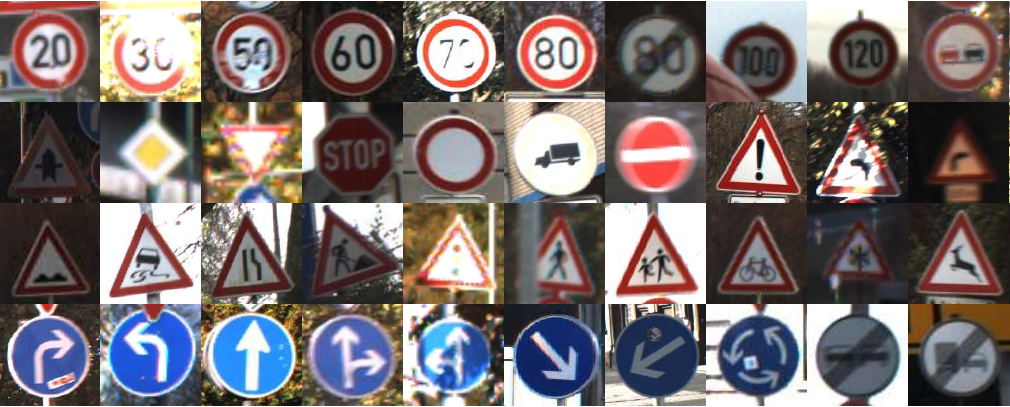
\includegraphics[width=0.7\textwidth]{images/intro/GTSRB}
		\end{center}
		\begin{center}
		\caption{\small{Algunas muestras de la base de datos GTSRB }}
		{\small{Fuente: \cite{Stallkamp2012}}}
		\end{center}
		\vspace{-1.5em}
		\end{figure}

		Los resultados sobre la base de datos GTSRB producieron un acierto del 99.46\% para el conjunto de imágenes evaluadas, \citep{Stallkamp2012}; sin embargo, desde entonces se han propuesto nuevas variantes de redes neuronales convolucionales, ya sea usando una funciones de activación diferentes, usando más capas en la red, mas filtros o introduciendo nuevos métodos de optimización. Lo importante del antecendente es que servirá como elemento de comparación para la investigación propuesta. 


	\newpage		
	\subsubsection
	{NACIONALES:}

		\citep{Vargas2015} en su tésis ”Implementación de un Sistema Inteligente para el Reconocimiento de Señales Preventivas de Seguridad vial", desarrolló un sistema basado enteramente en procesamiento de imágenes para la detección y el reconocimiento de señales de tránsito del tipo preventivas, usando para la detección la técnica de segmentación por color y luego un análisis por la forma y posteriormente para el reconocimiento se usó el algoritmo Speed Up Robust Features (SURF). Todo el proceso fue implementado utilizando la herramienta OpenCV, obteniendose un acierto del 88\% en un total de 100 señales evaluadas. De este antecedente se analizará la importancia de introducir la segmentación por color al modelo de reconocimiento que se pretende elaborar.
		\vskip 0.4cm

		\citep{Ayuque2016} en su tésis "Diseño de un sistema de clasificación de señales de tránsito vehicular utilizando redes neuronales convolucionales", diseñó 6 modelos de arquitecturas de redes convolucionales para clasificar diversas señales de tránsito de Alemania usando el dataset GTSRB, de los cuales el mejor resultado logró un acierto de 95.29\% en un total de 12630 señales evaluadas, cercano al 99.46\% \citep{Ciresan}. Lo importante del antecendente es que servirá como elemento de comparación para la investigación propuesta. 
		

%***********************************************************************************************************
%***********************************************************************************************************%***********************************************************************************************************

\section{Aprendizaje Profundo} 
	En los primeros días de la inteligencia artificial, el campo atacó y resolvió rápidamente problemas que son intelectualmente difíciles para los seres humanos pero relativamente sencillos para las computadoras, problemas que pueden describirse mediante una lista de reglas formales y matemáticas. El verdadero desafío para la inteligencia artificial fue y es resolver las tareas que son fáciles de realizar para las personas pero difíciles de describir de manera formal, problemas que resolvemos intuitivamente, que se sienten automáticos, como reconocer palabras, rostros u objetos en las imágenes \citep{Goodfellow-et-al-2016}.

	\vskip 0.4cm  
	Si bien aprendizaje automático(del inglés, {\bf machine learning}) se describe a menudo como una subdisciplina de la inteligencia artificial(IA), es mejor considerarla como la mejor técnica de la disciplina; es decir, es el campo de la IA que hoy en día muestra la mayor promesa al proporcionar herramientas que la industria y la sociedad pueden usar para producir algún cambio. En tal sentido,el aprendizaje automático toma algunas de las ideas centrales de la inteligencia artificial y las enfoca en resolver problemas del mundo real con redes neuronales diseñadas para imitar nuestra propia toma de decisiones; sin embargo, el {\bf aprendizaje profundo} o avanzado de máquinas (del inglés, {\bf deep learning}) se centra aún más estrechamente en un subconjunto de herramientas y técnicas del aprendizaje automático y los aplica a la solución de casi cualquier problema que requiera "pensamiento", ya sea humano o artificial.

	\vskip 0.4cm  
	El aprendizaje profundo es un enfoque específico utilizado para construir y entrenar redes neuronales para la toma de decisiones altamente prometedoras. Se considera que un algoritmo es profundo si los datos de entrada se pasan a través de una serie de no linealidades o transformaciones no lineales antes de que se emita. Este enfoque permitir que las computadoras aprendan de la experiencia y entiendan el mundo en términos de una jerarquía de conceptos, con cada concepto definido a través de su relación con conceptos más simples. Al reunir el conocimiento de la experiencia, este enfoque evita la necesidad de que los operadores humanos especifiquen formalmente todo el conocimiento que necesita la computadora. La jerarquía de conceptos permite que la computadora aprenda conceptos complicados mediante la construcción de los más simples. Si dibujamos un gráfico que muestra cómo estos conceptos se construyen uno encima del otro, el gráfico es profundo, con muchas capas. Por esta razón, este enfoque se conoce como el aprendizaje profundo de la inteligencia artificial \citep{Goodfellow-et-al-2016}.

	\vskip 0.4cm 
	El aprendizaje profundo elimina el hecho que se tenga que realizar una identificación manual de las características en los datos y, en cambio, depende del proceso de capacitación que tenga para descubrir los patrones útiles en los ejemplos de entrada. Esto hace que el entrenamiento de la red neuronal sea más fácil y más rápido \citep{Goodfellow-et-al-2016}. Las imágenes son un gran ejemplo de cómo funciona esto, ya que contienen muchos elementos diferentes y no es fácil para nosotros comprender cómo una computadora, con su mente o proceso centrado en el cálculo y direccionado en un solo sentido, puede aprender a interpretarlas de la misma manera que nosotros. Pero el aprendizaje profundo se puede aplicar a cualquier forma de datos (señales de máquina, audio, video, voz, palabras escritas) para producir conclusiones que parecen haber sido alcanzadas por simples humanos.

	\vskip 0.4cm 
	%\newpage
	Por el contrario, la mayoría de los algoritmos modernos de machine learning se consideran "poco profundos" porque la entrada solo puede abarcar unos pocos niveles de llamadas en subrutinas. El rendimiento de estos algoritmos simples de aprendizaje automático depende en gran medida de la presentación de los datos que se les proporcionan. Por ejemplo, cuando se usa la regresión logística para recomendar una cesárea, el sistema de IA no examina al paciente directamente. En cambio, el médico le dice al sistema varias piezas de información relevante, como la presencia o ausencia de una cicatriz uterina. Cada pieza de información incluida en la representación del paciente se conoce como una característica. La regresión logística aprende cómo cada una de estas características del paciente se correlaciona con diversos resultados. Sin embargo, no puede influir en cómo se definen las características de todos modos. Si a la regresión logística se le realizara una resonancia magnética del paciente, en lugar del informe formal del médico, no sería capaz de hacer predicciones útiles. Los píxeles individuales en una exploración de la resonancia tienen una correlación insignificante con cualquier complicación que pueda ocurrir durante el parto. Esta dependencia de las representaciones es un fenómeno general que aparece no solo en la vida cotidiana sino también en las ciencias de la computación. En tal sentido, operaciones como buscar una colección de datos puede avanzar exponencialmente más rápido si la colección está estructurada e indexada de forma inteligente. La gente puede realizar fácilmente números aritméticos arábigos, pero encuentra que la aritmética en números romanos consume mucho más tiempo. No es sorprendente que la elección de la representación tenga un enorme efecto en el rendimiento de los algoritmos de aprendizaje automático \citep{Goodfellow-et-al-2016}.

	\vskip 0.4cm 
	Para muchas tareas, sin embargo, es difícil saber qué características se deben extraer. Por ejemplo, un programa para detectar automóviles en fotografías. Se sabe que los autos tienen ruedas, por lo que sería importante utilizar la presencia de una rueda como característica. Desafortunadamente, es difícil describir exactamente cómo es una rueda en términos de valores de píxel. Una rueda tiene una geometría simple, pero su imagen puede verse complicada por las sombras que caen sobre la rueda, el sonido de las partes metálicas de la rueda, el guardabarros del automóvil o un objeto en el primer plano que oscurece la rueda, y así sucesivamente. 

	\vskip 0.4cm 
	Una solución a este problema es utilizar el aprendizaje automático para descubrir no solo el mapeo que inicia en la representación hasta el resultado sino también la representación en sí misma. Este enfoque se conoce como aprendizaje representativo(del inglés, {\bf representation learning}). Las representaciones aprendidas a menudo dan como resultado un rendimiento mucho mejor que el que se puede obtener con representaciones diseñadas a mano. También permiten que los sistemas de IA se adapten rápidamente a nuevas tareas, con una intervención humana mínima. Un algoritmo de aprendizaje de representación puede descubrir un conjunto de características para una tarea simple en minutos o para una tarea compleja en horas. El diseño manual de funciones para una tarea compleja requiere una gran cantidad de tiempo humano y esfuerzo; puede llevar décadas para toda una comunidad de investigadores, \citep{Goodfellow-et-al-2016}.
	\vskip 0.4cm 
	Al diseñar algoritmos para el aprendizaje de características, el objetivo suele ser separar los factores de variación que explican los datos observados. En este contexto, se usa la palabra "factores" simplemente para referirse a fuentes de influencia separadas; los factores generalmente no se combinan por multiplicación. Tales factores a menudo no son cantidades que se observan directamente. En cambio, pueden existir como objetos no observados o fuerzas no observadas en el mundo físico que afectan las cantidades observables. También pueden existir como constructores en la mente humana que proporcionan una simplificación útil de las explicaciones o causas inferidas de los datos observados. Pueden considerarse como conceptos o abstracciones que nos ayudan a dar sentido a la rica variabilidad de los datos. Al analizar una grabación de voz, los factores de variación incluyen la voz del hablante, su sexo, su acento y las palabras que están hablando. Al analizar la imagen de un automóvil, los factores de variación incluyen la posición del automóvil, su color y el ángulo y el brillo del sol.
	\vskip 0.4cm 
	Una fuente importante de dificultad en muchas aplicaciones de inteligencia artificial del mundo real es que muchos de los factores de variación influyen en cada pieza de datos que podemos observar. Los píxeles individuales en una imagen de un automóvil rojo pueden ser muy cercanos al negro en la noche. La forma de la silueta del automóvil depende del ángulo de visión. La mayoría de las aplicaciones nos exigen separar los factores de variación y descartar las que no nos interesan. Por supuesto, puede ser muy difícil extraer tales características abstractas de alto nivel a partir de datos en bruto. Muchos de estos factores de variación, como el acento de un hablante, solo se identifican mediante una comprensión sofisticada y casi humana de los datos. Cuando es casi tan difícil obtener una representación como para resolver el problema original, el aprendizaje de la representación, a primera vista, no parece ayudarnos.
	\vskip 0.4cm 
	El aprendizaje profundo resuelve este problema central en el aprendizaje representativo mediante la introducción de representaciones que se expresan en términos de otras representaciones más simples. El aprendizaje profundo permite a la computadora construir conceptos complejos a partir de conceptos más simples. La Figura 2.2 muestra cómo un sistema de aprendizaje profundo puede representar el concepto de una imagen de una persona combinando conceptos más simples, como esquinas y contornos, que a su vez se definen en términos de bordes.
		\begin{figure}[H]
		\begin{center}
		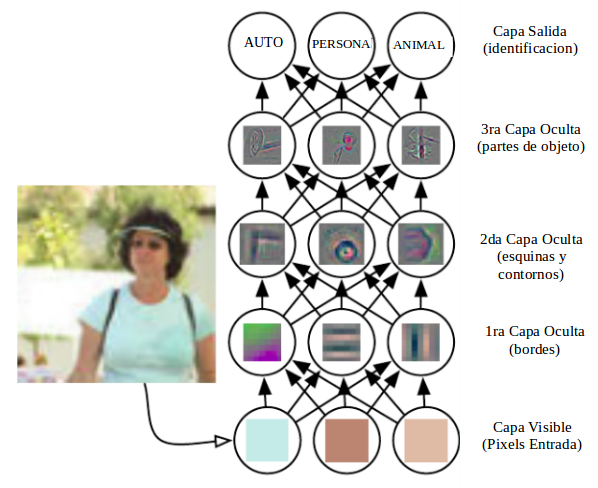
\includegraphics[width=0.7\textwidth]{images/marcoteorico/deepExam}
		\end{center}
		\begin{center}
		\caption{\small{Ilustración de un modelo de aprendizaje profundo}}
		\vskip -0.25cm
		{\small{Fuente: Elaboración propia}}
		\end{center}
		\vspace{-1.5em}
		\end{figure}
	\vskip 0.4cm 
	La idea de aprender la representación correcta de los datos proporciona una perspectiva para el aprendizaje profundo.\citep{Goodfellow-et-al-2016}. Otra perspectiva del aprendizaje profundo es que la profundidad permite que la computadora aprenda un programa de computadora de varios pasos. Cada capa de la representación se puede considerar como el estado de la memoria del computador después de ejecutar otro conjunto de instrucciones en paralelo. Las redes con mayor profundidad pueden ejecutar más instrucciones en secuencia. Las instrucciones secuenciales ofrecen gran poder porque las instrucciones posteriores pueden referirse a los resultados de instrucciones anteriores. De acuerdo con esta visión del aprendizaje profundo, no toda la información en las activaciones de una capa necesariamente codifica los factores de variación que explican la entrada. La representación también almacena información del estado que ayuda a ejecutar un programa el cual puede dar sentido a la entrada. Esta información de estado podría ser análoga a un contador o puntero en un programa informático tradicional. No tiene nada que ver con el contenido de la entrada específicamente, pero ayuda al modelo a organizar su procesamiento.
	\vskip 0.4cm 
	Hay dos formas principales de medir la profundidad de un modelo, \citep{Goodfellow-et-al-2016}. La primera vista se basa en la cantidad de instrucciones secuenciales que se deben ejecutar para evaluar la arquitectura. Podemos considerar esto como la longitud de la ruta más larga a través de un diagrama de flujo que describe cómo calcular cada una de las salidas del modelo a partir de sus entradas. Otro enfoque, utilizado por modelos probabilísticos profundos, considera que la profundidad de un modelo no es la profundidad del gráfico computacional sino la profundidad del gráfico que describe cómo los conceptos se relacionan entre sí. En este caso, la profundidad del diagrama de flujo de los cálculos necesarios para calcular la representación de cada concepto puede ser mucho más profunda que la gráfica de los conceptos mismos. Esto se debe a que la comprensión del sistema de los conceptos más simples puede ser refinado dada la información sobre conceptos más complejos.
	\vskip 0.4cm 
	Debido a que no siempre está claro cuál de estos dos puntos de vista (la profundidad del gráfico computacional o la profundidad del gráfico de modelado probabilístico) es más relevante, y debido a que diferentes personas eligen diferentes conjuntos de elementos más pequeños para construir sus gráficos, no hay un solo valor correcto para la profundidad de una arquitectura, así como no hay un solo valor correcto para la longitud de un programa de computadora. Tampoco hay consenso sobre la profundidad que requiere un modelo para calificar como "profundo", \citep{Goodfellow-et-al-2016}. Sin embargo, el aprendizaje profundo puede considerarse con seguridad como el estudio de modelos que implican una mayor cantidad de composición de funciones o conceptos aprendidos en comparación con el aprendizaje automático tradicional.
	\vskip 0.4cm 
	En resumen, el aprendizaje profundo, es un enfoque a la IA. Específicamente, es un tipo de aprendizaje automático, una técnica que permite que los sistemas computacionales mejoren con la experiencia y los datos. En este sentido, se puede sostener que el aprendizaje automático es el único enfoque viable para construir sistemas de inteligencia artificial que puedan operar en entornos complicados del mundo real y el aprendizaje profundo es un tipo particular de aprendizaje automático que logra gran poder y flexibilidad al representar el mundo como una jerarquía de conceptos anidados, con cada concepto definido en relación con conceptos más simples y representaciones más abstractas calculadas en base a representaciones menos abstractas. La siguiente imagen es un diagrama de Venn que muestra cómo el aprendizaje profundo es una especie de aprendizaje de representación, que a su vez es una especie de aprendizaje automático, que se utiliza para muchos, pero no todos los enfoques de la IA. 

	\begin{figure}[H]
		\begin{center}
		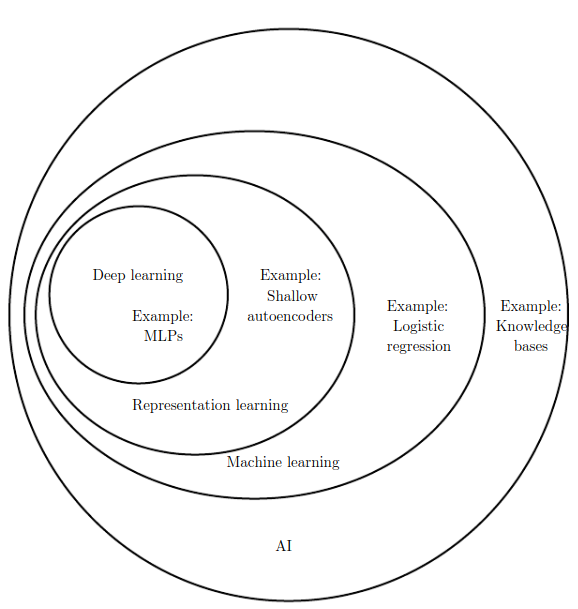
\includegraphics[width=0.8\textwidth, height=12.5cm]{images/marcoteorico/venn_diag}
		\end{center}
		\begin{center}
		\vskip -0.1cm
		\caption{\small{Diagrama de Venn donde cada sección incluye un ejemplo de una tecnología de IA(ilustra la relación entre estas diferentes disciplinas de la IA)}}
		{\small{Fuente: \cite{Goodfellow-et-al-2016}}}
		\end{center}
		\vspace{-1.5em}
		\end{figure}

\section{Red Convolucional} 

	Nueve de cada diez veces, cuando se escucha que el aprendizaje profundo rompe una nueva barrera tecnológica, las redes neuronales convolucionales están involucradas. También llamados CNN(del inglés , {\bf Convolutional Neural Networks}) o  {\bf ConvNets}, estas son las preferidas del campo de redes neuronales profundas. Han aprendido a clasificar las imágenes en categorías incluso mejor que los humanos en algunos casos, \citep{Rohrer}.
	
	\vskip 0.4cm  
	Las arquitecturas de redes convolucionales siempre suponen explícitamente que las entradas deben ser mapeadas en forma de imágenes, lo que nos permite configurar parte inicla de las propiedades o características de la arquitectura a diseñar.  Debido a esta característica la limitación de las ConvNets radica en que solo capturan patrones espaciales locales en datos. Es decir, si no se puede hacer que los datos se vean como una imagen, las ConvNets son practicamente muy poco útiles,\citep{Rohrer}.

	\vskip 0.4cm  
	Las redes neuronales convolucionales son muy similares a las redes neuronales ordinarias, están formadas por neuronas que tienen pesos y biases(sesgos) que se pueden aprender durante el entrenamiento de estas. Cada neurona recibe algunas entradas y realiza operaciones matemáticas. Toda la red expresa una única función de puntuación diferenciable: desde el contenido de los píxeles de la imagen en un extremo(entrada) hasta los puntajes que definen la clase o resultado correspondiente en el otro extremo(salida).

	\begin{figure}[H]
	\begin{center}
	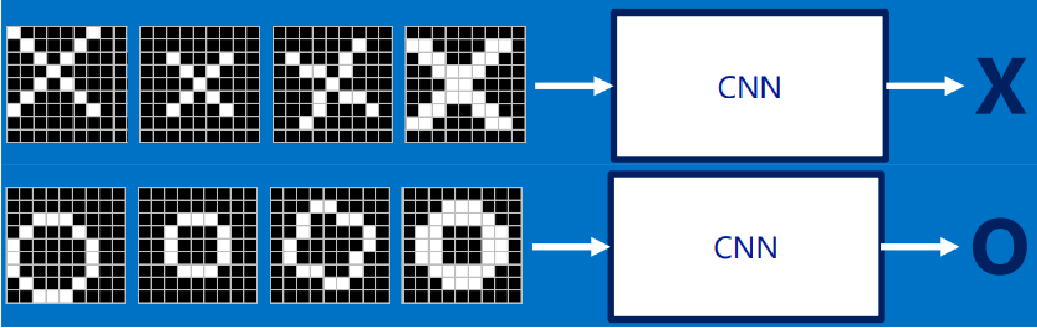
\includegraphics[width=0.7\textwidth]{images/marcoteorico/entr_salida}
	\end{center}
	\begin{center}
	\caption{\small{Entrada y salida de una CNN}}
	\vskip -0.25cm
	{\small{Fuente: \cite{Rohrer}}}
	\end{center}
	\vspace{-1.5em}
	\end{figure}

	El resultado de las CNNs es que pueden encontrar si una característica está en una imagen sin preocuparse exactamente de donde está. Esto ayuda a resolver el problema de las computadoras al comparar imágenes de manera hiper-literal, es decir, que coincida pixel a pixel para que se trate de imágenes iguales.

	\begin{figure}[H]
	\begin{center}
	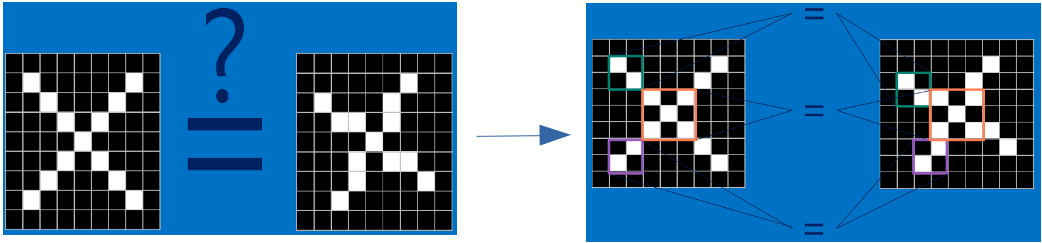
\includegraphics[width=0.8\textwidth]{images/marcoteorico/literalcomp}
	\end{center}
	\begin{center}
	\caption{\small{Analisis de una CNN}}
	\vskip -0.25cm
	{\small{Fuente: \cite{Rohrer}}}
	\end{center}
	\vspace{-1.5em}
	\end{figure}

	Una ConvNet se caracteriza por tener una secuencia de capas donde cada una de estas transforma un volumen de activaciones en otro nuevo a través de funciones y el aprendizaje profundo se produce cuando se utilizan varias de estas capas variando los parámetros de configuación dentro y entre dichas capas. 
	\vskip 0.4cm  
	Existen dos conjuntos de terminologías para describir estas capas. Una es cuando la red convolucional es vista como un número largo de capas simples y cada paso del procesamiento se considera como una capa en sí misma. Otra terminología es cuando la red convolucional es vista como un número pequeño de capas relativamente complejas, donde cada capa tiene multiples etapas. En esta terminología, existe un mapeo directo entre los volumenes de activaciones y las capas de red. En esta investigación se usará esta terminología.

	
	\begin{figure}[H]
	\begin{center}
	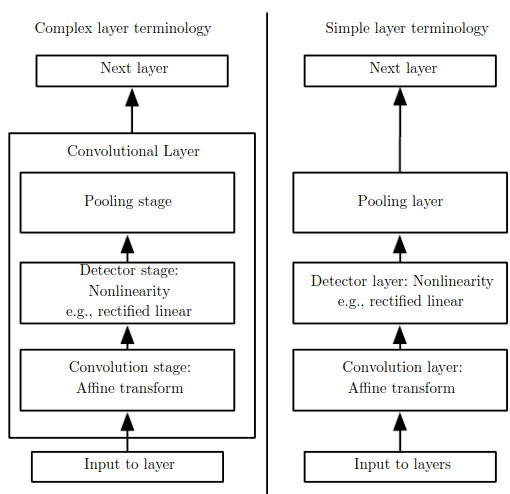
\includegraphics[width=0.6\textwidth]{images/marcoteorico/types}
	\end{center}
	\begin{center}
	\caption{\small{Terminología de capas complejas(izquierda) y de capas simples(derecha)}}
	{\small{Fuente: \cite{Goodfellow-et-al-2016}}}
	\end{center}
	\vspace{-1.5em}
	\end{figure}
	
	\subsection{Capa Convolucional}

		Los parámetros de la capa convolucional consisten basicamente en dos datos. La entrada y todo lo que respecta a un conjunto de filtros(también denomidados kernels) cuyos valores se aprenden, es decir, empiezan con datos aleatorios y conforme avance el entrenamiento se van alterando. 
		\vskip 0.3cm 
		\subsubsection {Etapa de Convolución} 
		  
		Para el proceso convolucional cada filtro es pequeño espacialmente (a lo ancho y alto), incluso se extiende a través de la profundidad total del volumen de entrada(imagen). Por ejemplo, un filtro típico en una primera capa de una ConvNet podría tener un tamaño de 5x5x3 (es decir, 5 píxeles de ancho y alto, y 3 de profundidad debido a que los canales de color - RGB). Durante el proceso hacia adelante, se desliza (más precisamente, convolve) cada filtro a través del ancho y alto(incluso produnfidad) del volumen de entrada para calcular los productos de puntos entre las entradas del filtro y la entrada en cualquier posición.

		\begin{figure}[H]
		\begin{center}
		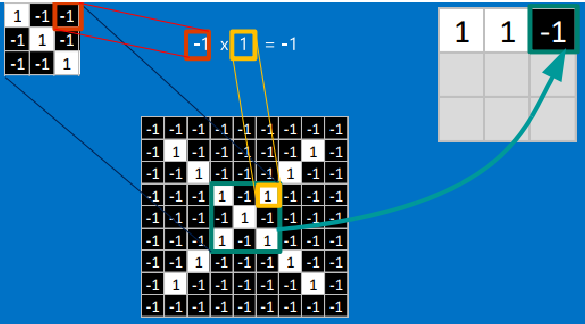
\includegraphics[width=0.75\textwidth]{images/marcoteorico/generate_filt1}
		\end{center}
		\begin{center}
		\caption{\small{Convolucion entre el filtro y parte de la imagen}}
		\vskip -0.25cm
		{\small{Fuente: \cite{Rohrer}}}
		\end{center}
		\vspace{-1.9em}
		\end{figure}

		\begin{figure}[H]
		\begin{center}
		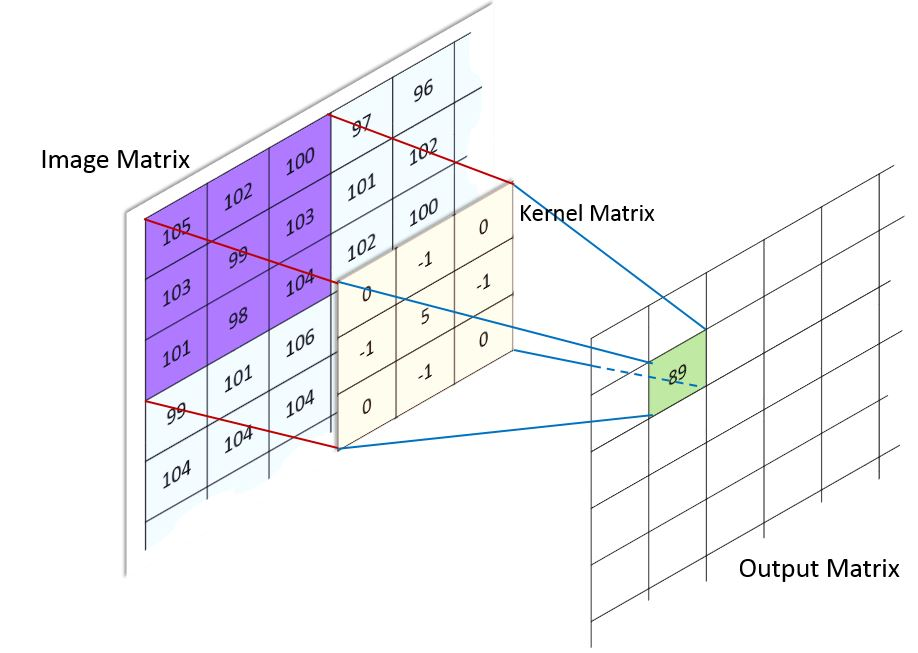
\includegraphics[width=0.75\textwidth]{images/marcoteorico/Convolution_calculation1}
		\end{center}
		\begin{center}
		\caption{\small{Posicionamiento del kernel/filtro por pixel}}
		{\small{Fuente: Fuente: Elaboración propia}}
		\end{center}
		\vspace{-1.9em}
		\end{figure}

		A medida que deslizamos el filtro sobre el ancho y la altura del volumen de entrada produciremos un mapa de activación bidimensional que proporciona las respuestas de ese filtro en cada posición espacial. Es decir, el proceso en esta capa consiste en calcular la coincidencia de un filtro con una parte de la imagen,y para conseguirlo simplemente se multiplica cada píxel en el filtro por el valor del píxel en la imagen. Para luego, sumar las respuestas y dividirlas por el número total de píxeles en el filtro.

		\begin{figure}[H]
		\begin{center}
		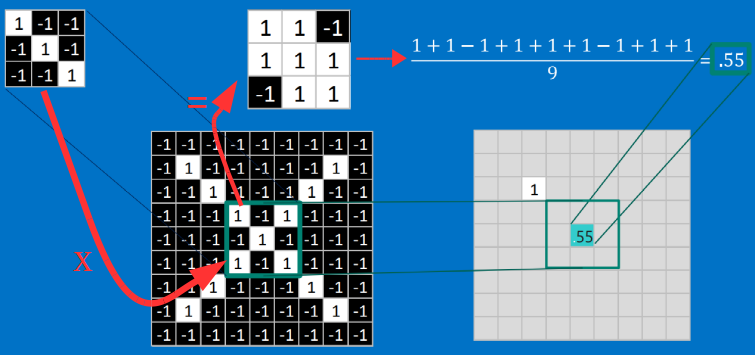
\includegraphics[width=0.75\textwidth]{images/marcoteorico/conv_filt1}
		\end{center}
		\begin{center}
		\caption{\small{Proceso matemático convolucional}}
		{\small{Fuente:\cite{Rohrer}}}
		\end{center}
		\vspace{-1.5em}
		\end{figure}

		\begin{figure}[H]
		\begin{center}
		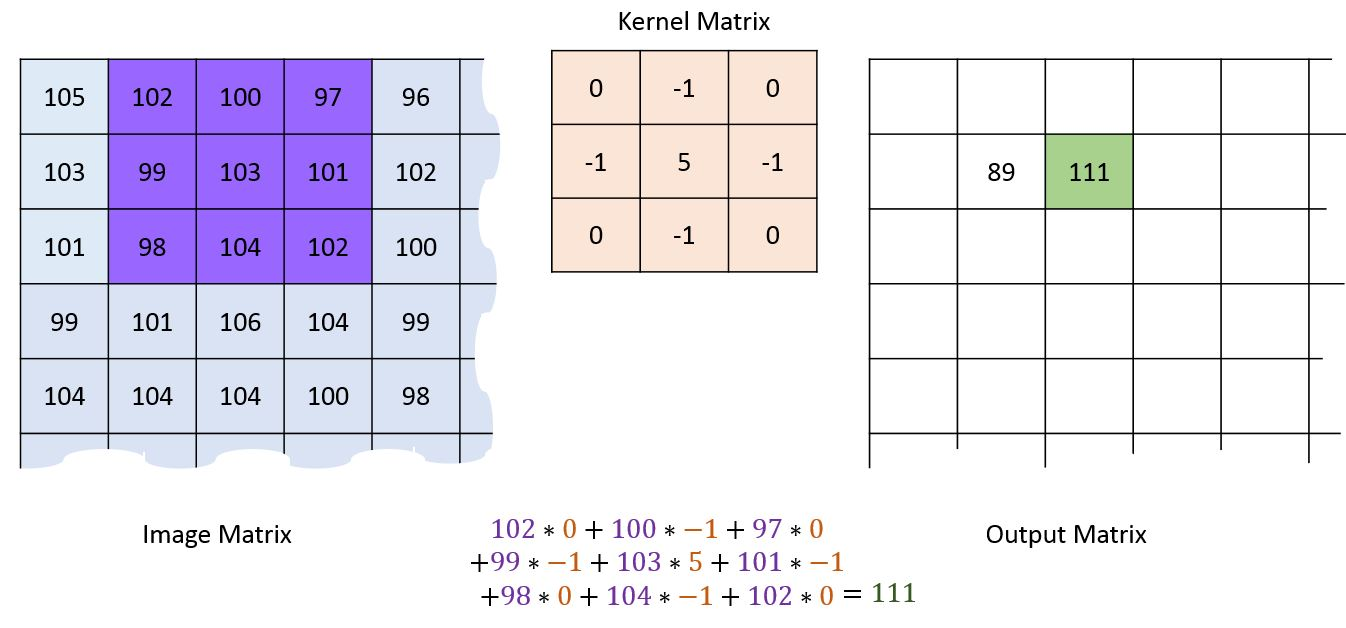
\includegraphics[width=0.75\textwidth]{images/marcoteorico/Convolution_calculation2}
		\end{center}
		\begin{center}
		\caption{\small{Cálculo Convolucional}}
		{\small{Fuente: Fuente: Elaboración propia}}
		\end{center}
		\vspace{-1.9em}
		\end{figure}

		Cada filtro puede ser representado como una neurona de salida, cuyo valor se halla usando la sumatoria de pesos como se muestra en la figura 11. Intuitivamente, la red aprenderá los filtros que se activan cuando ven algún tipo de característica visual, como un borde o contorno en alguna orientación específica. 
		
		\vskip 0.4cm  
		
		La convolución aprovecha tres ideas importantes que pueden ayudar a mejorar un sistema de aprendizaje automático: {\bf interacciones dispersas}, {\bf uso compartido de parámetros} y {\bf representaciones equivalentes}.
		
		\vskip 0.4cm  
		Las capas de redes neuronales tradicionales usan la multiplicación de matrices mediante una matriz de parámetros con un parámetro separado que describe la interacción entre cada unidad de entrada y cada unidad de salida. Esto significa que cada unidad de salida interactúa con cada unidad de entrada. Sin embargo, las redes convolucionales suelen tener {\bf interacciones dispersas} (también conocidas como conectividad dispersa o ponderaciones dispersas). Esto se logra haciendo que el kernel sea más pequeño que la entrada. Por ejemplo, al procesar una imagen, la imagen de entrada puede tener miles o millones de píxeles, pero podemos detectar características pequeñas y significativas, como bordes con núcleos que ocupan solo decenas o cientos de píxeles. Esto significa que necesitamos almacenar menos parámetros, lo que reduce los requisitos de memoria del modelo y mejora su eficiencia estadística. También significa que el cálculo de la salida requiere menos operaciones.
		
		\begin{figure}[H]
		\begin{center}
		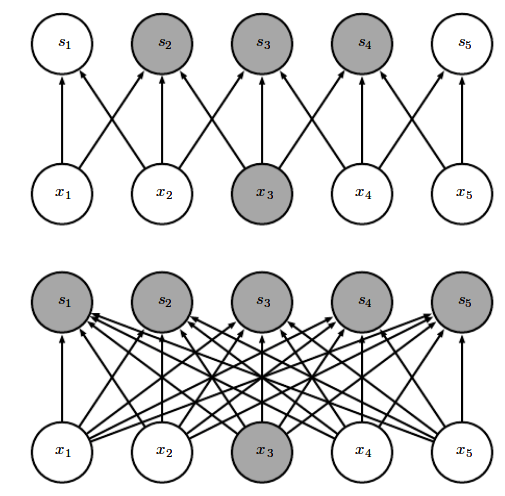
\includegraphics[width=0.5\textwidth]{images/marcoteorico/sparceCon}
		\end{center}
		\begin{center}
		\caption{\footnotesize \small{Conectividad dispersa vs No Dispersa}}
		\vskip -0.3cm  
		{\small{Fuente:\cite{Goodfellow-et-al-2016}}}
		\end{center}
		\vspace{-1.5em}
		\end{figure} 	

		Estas mejoras en la eficiencia suelen ser bastante grandes. Si hay entradas y salidas, la multiplicación de la matriz requiere $m \times n$ parámetros, y los algoritmos utilizados en la práctica por ejemplo tienen complejidad de tiempo de ejecución $O(m \times n)$. Si limitamos el número de conexiones que cada salida puede tener a {\textit k}, entonces el enfoque dispersamente conectado requiere solo $k \times n$ parámetros y $O(k \times n)$ en tiempo de ejecución. Para muchas aplicaciones prácticas, es posible obtener un buen rendimiento en la tarea de aprendizaje automático mientras se mantienen {\textit k} distintos órdenes de magnitud menores que {\textit m}. Para demostraciones gráficas de conectividad dispersa, vea la figura 2.10, donde se resalta una unidad de entrada $x_{3}$, y las unidades de salida que son afectadas por esta unidad. (Arriba) Cuando {\bf {\textit {s}}} está formado por convolución con un kernel de ancho 3, solo tres salidas se ven afectadas por {\bf \textit  x}. (Abajo) Cuando {\bf \textit s} está formado por la multiplicación de la matriz, la conectividad ya no es dispersa, por lo que todos los resultados se ven afectados por $x_{3}$.

		\vskip 0.4cm  
		En una red convolucional profunda, las unidades en las capas más profundas pueden interactuar indirectamente con una porción más grande de la entrada. Esto permite que la red describa de manera eficiente las interacciones complicadas entre muchas variables mediante la construcción de tales interacciones a partir de bloques de construcción simples que describen cada una de ellas. Entonces, aunque las conexiones directas en una red convolucional son muy dispersas, las unidades en las capas más profundas pueden conectarse indirectamente a la totalidad o a la mayoría de la imagen de entrada,\citep{Goodfellow-et-al-2016}.
		
		\vskip 0.4cm  
		
		El uso {\bf compartido de parámetros} hace referencia al uso del mismo parámetro para más de una función en un modelo. En una red neuronal tradicional, cada elemento de la matriz de pesos se usa exactamente una vez cuando se calcula la salida de una capa. Se multiplica por un elemento de la entrada y luego nunca se vuelve a visitar. Como sinónimo de compartición de parámetros, se puede decir que una red tiene ponderaciones vinculadas, porque el valor de la ponderación aplicada a una entrada está vinculado al valor de una ponderación aplicada a otra parte. En una red neuronal convolucional, cada miembro del kernel se utiliza en cada posición de la entrada (excepto tal vez algunos de los píxeles de los bordes, dependiendo de las decisiones de diseño con respecto al límite). El uso compartido de parámetros utilizado por la operación de convolución significa que en lugar de aprender conjuntos de parámetros para cada ubicación por separado, aprendemos un solo conjunto, \citep{Goodfellow-et-al-2016}.
		\vskip 0.4cm  

		En el caso de la convolución, la forma particular de compartir los parámetros hace que la capa tenga una propiedad llamada {\bf representaciones equivalentes}. Decir que una función es equivalente significa que si la entrada cambia, la salida cambia de la misma manera.
		La convolución crea un mapa en 2-D de donde aparecen ciertas características en la entrada. Si movemos el objeto en la entrada, su representación se moverá la misma cantidad en la salida. Esto es útil cuando sabemos que se utiliza alguna función de un número pequeño de píxeles vecinos cuando se aplica a ubicaciones de entrada múltiples. Por ejemplo, al procesar imágenes, es útil detectar bordes en la primera capa de una red convolucional. Los mismos bordes aparecen más o menos en todas partes en la imagen, por lo que es práctico compartir los parámetros en toda la imagen.

		\begin{figure}[H]
		\begin{center}
		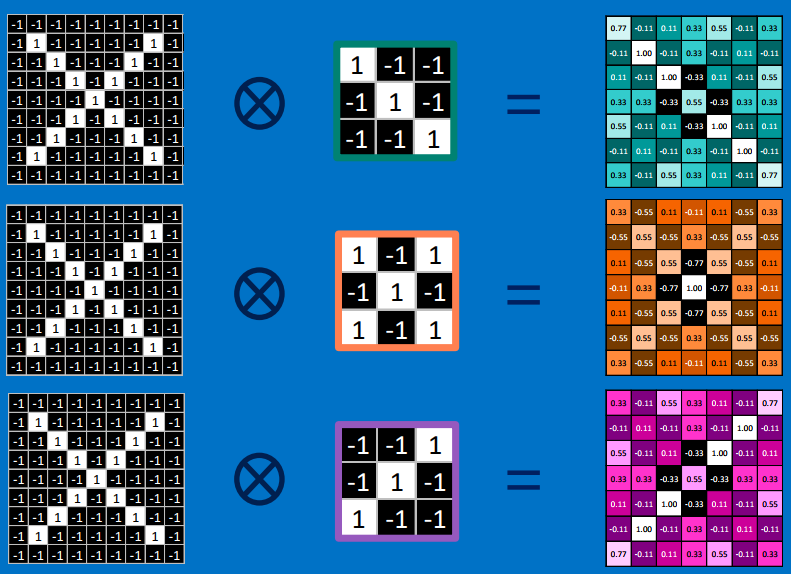
\includegraphics[width=0.6\textwidth]{images/marcoteorico/result_conv}
		\end{center}
		\begin{center}
		\vskip 0.1cm  
		\caption{\small{Resultado de Convolución(conjunto de mapas de activación. generado a partir de 3 filtros para 3 carecteristicas: diagonal derecha, cruzamiento central y diagonal izquierda). Simbolo de convolución: $\otimes$}}
		\vskip -0.1cm  
		{\small{Fuente: \cite{Rohrer}}}
		\end{center}
		\vspace{-1.9em}
		\end{figure}

		En resumen, se tiene un conjunto completo de "n"  filtros en cada capa convolucional(determinando la profundidad de la capa) y cada uno de estos filtros producirá un mapa de activación bidimensional por separado. Apilaremos estos mapas de activación a lo largo de la dimensión de profundidad y produciremos el volumen de salida, es decir el resultado es un conjunto de imágenes que muestran un versión filtrada de la imagen original resaltando características o patrones importantes de ella, como puede ser visto en la figura 2.11.

		\vskip 0.4cm  
		Cabe resaltar que para la construcción de un filtro o kernel, es necesario considerar tres aspectos importantes: la extensión espacial (spatial extent), el paso (stride) y la cantidad de zero a rellenar (zero-padding).
		\newpage
		
		\begin{enumerate}
			\item La extensión espacial es el tamaño del filtro, comúnmente es de tamaño impar tanto en largo y ancho.
			
			\item El stride es otra pieza del bloque de construcción básico de los filtros convolucionales. Este representa el {\textit 'paso'} en la operación de convolución indicando cuánto es que se debe desplazar un filtro en una imagen con cada paso. El filtro se desliza sobre la imagen, se detiene en cada longitud de salto y realiza las operaciones necesarias en ese paso.

				\begin{figure}[H]
				\begin{center}
				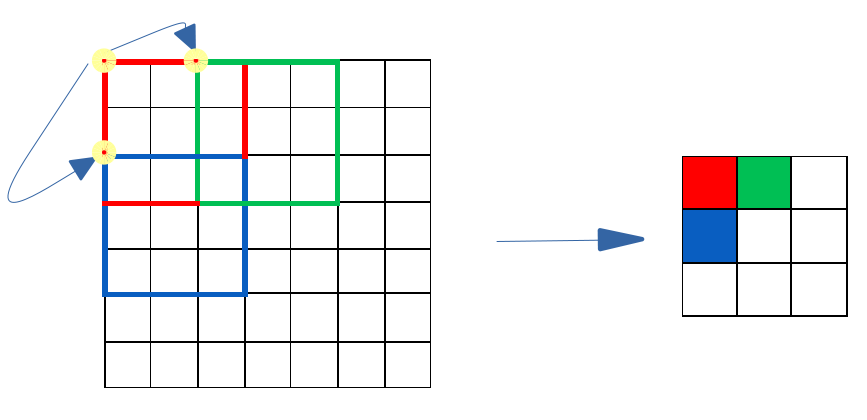
\includegraphics[width=0.65\textwidth]{images/marcoteorico/stride}
				\end{center}
				\begin{center}
				\caption{\small{Imagen con stride igual a 2, para el filtro tanto en largura como anchura}}
				\vspace{-0.5em}
				{\small{Fuente: Elaboración propia}}
				\end{center}
				\vspace{-1.9em}
				\end{figure}
			\item Zero-padding agrega ceros alrededor del borde de una imagen.
				\begin{figure}[H]
				\begin{center}
				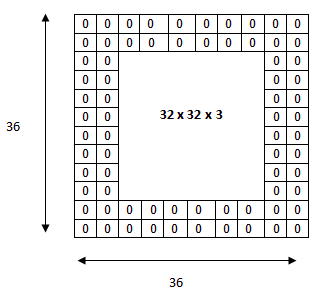
\includegraphics[width=0.4\textwidth]{images/marcoteorico/PAD2}
				\end{center}
				\begin{center}
				\caption{\small{Ejemplo de zero-padding con tamaño 2}}
				\vspace{-0.5em}
				{\small{Fuente: Elaboración propia}}
				\end{center}
				\vspace{-1.9em}
				\end{figure}

				Los principales beneficios del relleno son los siguientes:
				\begin{itemize}
				\item Le permite usar una capa de convolución sin necesariamente reducir la altura y el ancho de los volúmenes. Esto es importante para construir redes más profundas, ya que de lo contrario la altura / ancho se reduciría a medida que se avanza hacia capas más profundas.
				\item Nos ayuda a mantener más información en el borde de una imagen. Sin relleno, muy pocos valores en la siguiente capa se verían afectados por los píxeles como los bordes de una imagen.
				\end{itemize}
			
		\end{enumerate}
		%\vskip 0.4cm  

		\noindent Cada capa convolucional recibe como dato de entrada llos parámetros:
		${W_{0}}\times{H_{0}}\times{D_{0}}$ \newline
		Produce un dato de salida con los siguiente parámetros: ${W_{1}}\times{H_{1}}\times{D_{1}}$\newline
		Estas salidas, son influenciadas por la manera de configuración de los filtros.\newline
		\vspace{-2em} 
		
		\begin{minipage}[t]{0.5\textwidth}
		En el que:
		\begingroup\makeatletter\def\f@size{12.4}\check@mathfonts
		\begin{center}
		 ${W_{1}} = \frac{{W_{0}} - F + 2P}{S} +1$ 
		\vskip 0.4cm 
		 ${H_{1}} = \frac{{H_{0}} - F + 2P}{S} +1$ 
		\vskip 0.4cm 
		 ${D_{1}} = K$ 
		 \end{center}
		\endgroup
		\end{minipage}
		%second column
		\begin{minipage}[t]{0.55\textwidth}
		Donde:
		\vskip 0.1cm 
		$W$ es el ancho (width) de la imagen, \vskip 0.4cm  
		$H$ es la altura (height) de la imagen,\vskip 0.4cm 
		$D$ es la profundidad (depth)de la imagen,\vskip 0.4cm 
		$F$ es la extensión espacial (spatial extent) del filtro,\vskip 0.4cm 
		$S$ es el paso (stride) del filtro,\vskip 0.4cm 
		$P$ es la cantidad de zero padding del filtro,\vskip 0.4cm 
		$K$ es el número de filtros (filters).\vskip 0.4cm 
		\end{minipage}
		\vskip 0.4cm 
		\noindent La ecuación de convolución de manera generalizada es:
		
		\begingroup\makeatletter\def\f@size{14.4}\check@mathfonts
		\begin{center}
		${conv_j^n} ={\sum_{k=1}^k x_k^n \times w_{kj} ^n + b_n}$
		\end{center}
		\endgroup
		
		En el que:\vskip 0.1cm
		\begin{itemize}
			\item $x,w,b$ son valores de entrada, pesos y biases(sesgos), respectivamente
			\item $n$ es el número de la capa
			\item $j$ es el número del filtro de salida
			\item $k$ es la cantidad de filtros en la capa $n-1$ o $n$
		\end{itemize}


		\begin{figure}[H]
		\begin{center}
		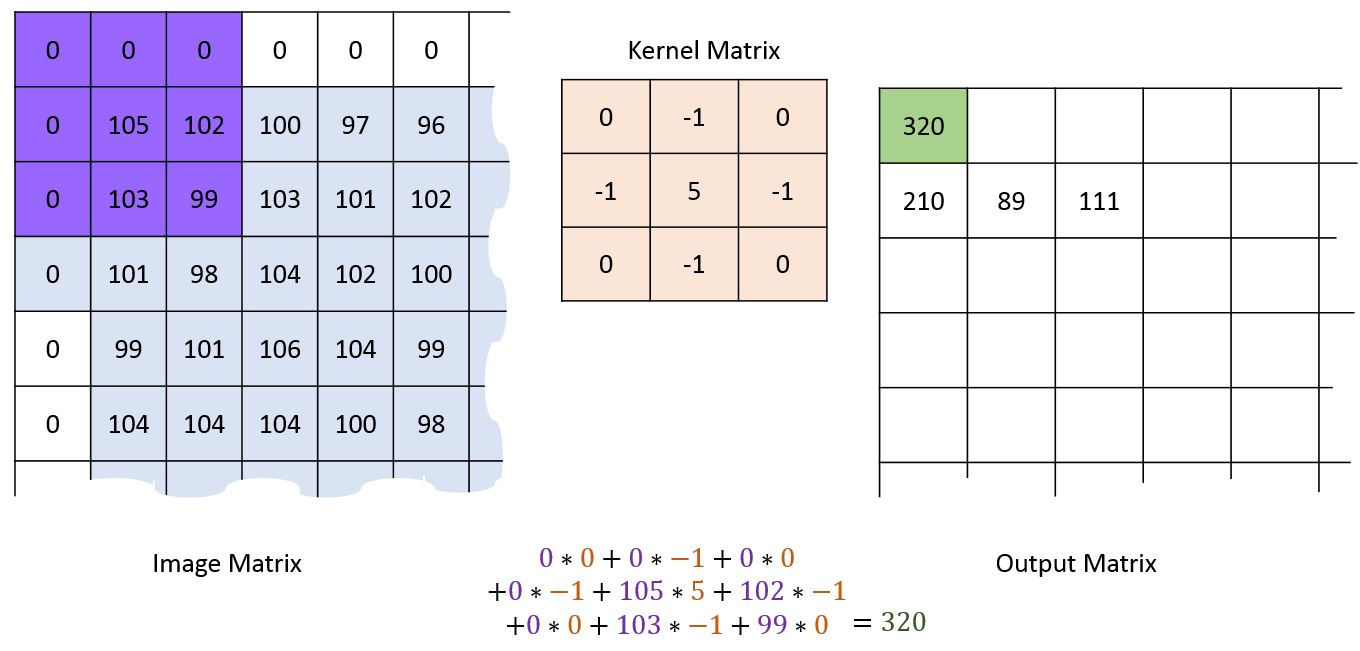
\includegraphics[width=0.75\textwidth]{images/marcoteorico/Convolution_calculation_borders}
		\end{center}
		\begin{center}
		\caption{\small{Ejemplo de filtro crado apartir de los 3 aspectos mencionados}}
		{\small{Fuente: Elaboración propia}}
		\end{center}
		\vspace{-1.9em}
		\end{figure}
 
	\subsubsection  {Capa ReLU(Rectified Linear Units)}
		\vskip 0.4cm 
		Debido al hecho que todas las capas en una red neuronal no son lineales. Después de calcular los valores para cada una de las neuronas en la red neuronal, colocamos estos valores a través de una función de activación. Una red neuronal artificial consiste básicamente en multiplicaciones y suma de matrices. Si solo utilizáramos estos cálculos lineales, podríamos apilarlos uno encima del otro y esa no sería una red muy profunda. Por lo tanto, a menudo se utiliza funciones de activación no lineales en cada capa de la red. Al apilar capas de funciones lineales y no lineales una encima de la otra, teóricamente podemos modelar cualquier problema.
		\vskip 0.4cm 
		Estas son las tres funciones de activación no lineal más populares:
		\begin{enumerate}
		\item[1)] Sigmoid (analiza un valor entre 0 y 1)  \vspace{-0.5em}
		\item[2)] TanH (analiza un valor entre -1 y 1) \vspace{-0.5em}
		\item[3)] ReLU (si el valor es negativo, se convierte en 0, de lo contrario, permanece igual) \vspace{-0.5em}
		\end{enumerate}

		\begin{figure}[H]
		\begin{center}
		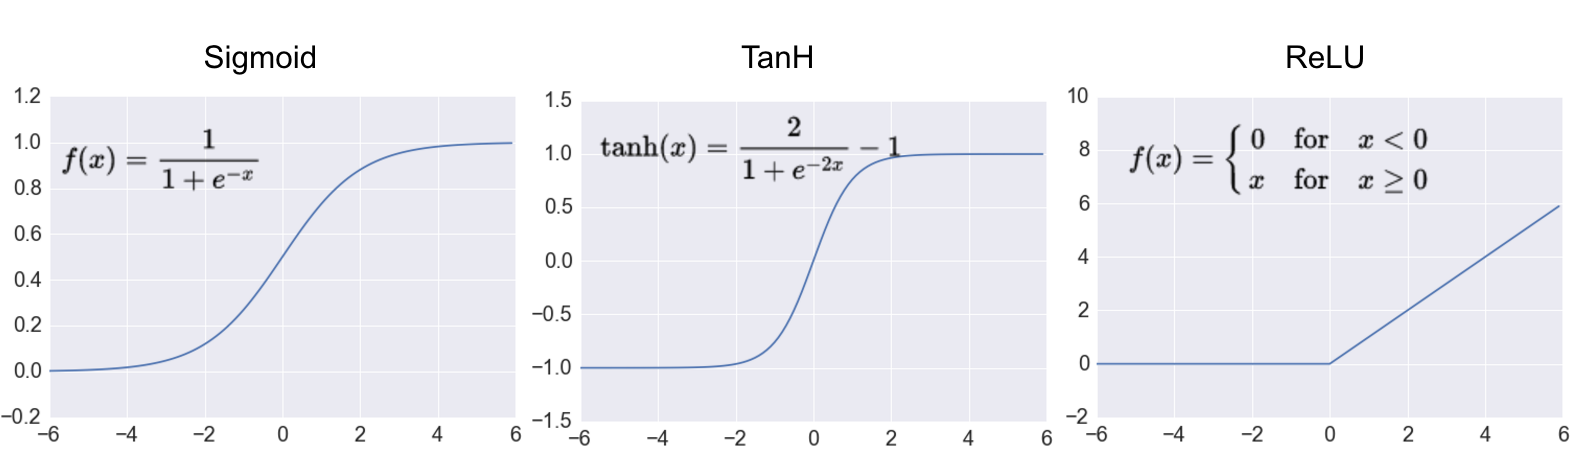
\includegraphics[width=0.8\textwidth]{images/marcoteorico/activfunct}
		\end{center}
		\begin{center}
		\caption{\small{Funciones de activación}}
		\vskip -0.2cm  
		{\small{Fuente: Elaboración propia}}
		\end{center}
		\vspace{-1.5em}
		\end{figure}

		Actualmente, ReLU es la función de activación no lineal más utilizada \citep{cs231n}. La razón principal de esto es porque la red puede entrenar mucho más rápido (debido a la eficiencia computacional) sin hacer una diferencia significativa en la precisión. También ayuda a aliviar el problema del gradiente de fuga, que es el problema donde las capas inferiores de la red entrenan muy lentamente porque el gradiente de optimización	disminuye exponencialmente a través de las capas. La capa ReLU aplica la función ${f(x)} = {max (0, x)} $ a todos los valores en el volumen de entrada. En términos básicos, esta capa simplemente cambia todas las activaciones negativas a 0. Esta capa aumenta las propiedades no lineales del modelo y la red global sin afectar los campos receptivos de la capa conv. El hecho de que entradas en la función de activación de valores menores o iguales a cero resulten cero, induce a la dispersión en las unidades ocultas, que según lo comentado anteriormente, produce representaciones dispersas las cuales se consideran más valiosas, \citep{RELU}. 
		
		\begin{figure}[H]
		\begin{center}
		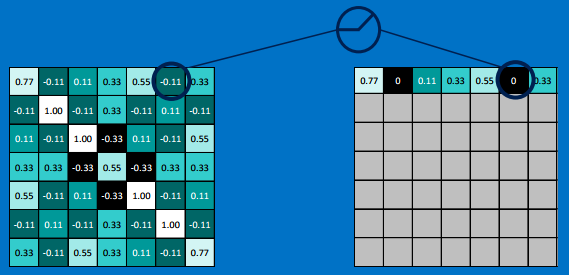
\includegraphics[width=0.8\textwidth, height=6cm]{images/marcoteorico/relu}
		\end{center}
		\begin{center}
		\caption{\small{Procedimiento de la función ReLU}}
		\vskip -0.2cm  
		{\small{Fuente: \cite{Rohrer}}}
		\end{center}
		\vspace{-1.5em}
		\end{figure}
		\vskip 0.4cm
		
		Es por ello que entre la capa(etapa) de convolucion y la capa(etapa) de pooling puede encontrarse la capa ReLU que esta compuesta por neuronas que poseen una funcion de activación llamada Función Lineal Rectificada que deriva de la función de activación sigmoidal, pero tiene mayores ventajas que esta última y tambien de la tangencial. Las activaciones de ReLU se sobreponen más fácilmente que los sigmoides, esto los prepara muy bien para ser utilizados en combinación con la técnica DROPOUT.
		
		\vskip 0.4cm 
	\subsubsection {Técnica Dropout}
		\vskip 0.4cm 
		Combinar las predicciones de muchos modelos diferentes es una forma muy exitosa de reducir los errores de prueba, pero parece ser demasiado costoso para las redes neuronales de gran tamaño debido a que pueden tardar varios días en entrenar. Sin embargo, dropout es una técnica de regularización que tiene por objetivo de reducir el sobreajuste que puede darse durante el entrenamiento de una red neuronal. Consiste en establecer a cero la salida de cada neurona oculta con una probabilidad 0.5(comúnmente). Las neuronas que se abandonan de esta manera no contribuyen al pase directo y no participan en las siguientes etapas de entrenamiento.

		\begin{figure}[H]
		\begin{center}
		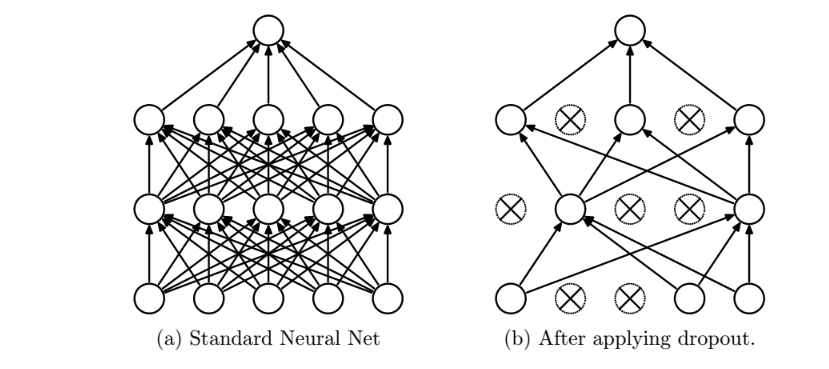
\includegraphics[width=0.8\textwidth]{images/marcoteorico/dropout_sample}
		\end{center}
		\begin{center}
		\caption{\small{En la izquierda la red neuronal común y a la derecha la red neuronal diluida producida por la aplicación de dropout}}
		{\small{\cite{AulaDNN}}}
		\end{center}
		\vspace{-1.5em}
		\end{figure}
		

		\vskip 0.4cm 
		Por lo tanto, cada vez que se presenta una entrada, la red neuronal muestra una arquitectura diferente, pero todas estas arquitecturas comparten ponderaciones. Esta técnica reduce las coadaptaciones complejas de las neuronas, ya que una neurona no puede depender de la presencia de otras neuronas particulares. Por lo tanto, se ve forzado a aprender características más robustas que son útiles en conjunción con muchos subconjuntos aleatorios diferentes de las otras neuronas.
		\begin{figure}[H]
		\begin{center}
		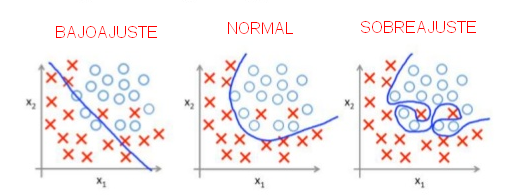
\includegraphics[width=0.8\textwidth]{images/marcoteorico/dropout}
		\end{center}
		\begin{center}
		\caption{\small{Procesos que pueden ocurrir durante entrenamiento. Dropout evita el sobreajuste}}
		\vskip -0.3cm  
		{\small{Fuente: Elaboración propia}}
		\end{center}
		\vspace{-1.5em}
		\end{figure}

		\vskip 0.4cm 
	\subsubsection {Capa de Agrupación(Pooling)}
		\vskip 0.4cm 

		Una variedad de cálculos que reducen la dimensionalidad de un mapa de características se conocen como agrupación. La agrupación, que se aplica a cada canal por separado, permitiendo que la red sea robusta e invariante a pequeños cambios y distorsiones. La capa Pooling(también conocida como una capa de reducción de resolución) combina o agrupa, un conjunto de valores en su campo receptivo en un menor número de valores. Puede ser configurado en función del tamaño de su campo receptivo (por ejemplo, 2 x 2) y en función a la operación de agrupamiento (por ejemplo, máximo-max o promedio-average), como se muestra en Fig. 2.19. Normalmente, la agrupación se produce en bloques que no se solapan (es decir, el paso o stride es igual al tamaño de la agrupación). Usualmente se usa una stride mayor que uno cuando se quiere que haya una reducción en la dimensión de la representación(mapa de características).

		\begin{figure}[H]
		\begin{center}
		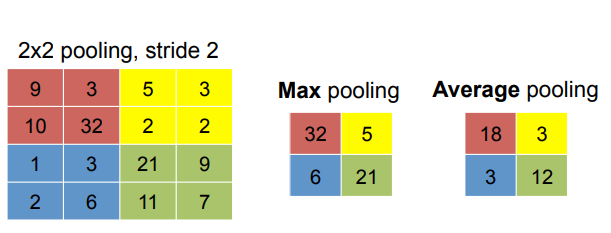
\includegraphics[width=0.8\textwidth]{images/marcoteorico/pooling}
		\end{center}
		\begin{center}
		\caption{\small{Formas de agrupamiento(pooling)}}
		\vskip -0.2cm  
		{\small{Fuente: \cite{caffe}}}
		\end{center}
		\vspace{-1.5em}
		\end{figure}

		Después de algunas capas ReLU, es común optar por aplicar una capa de agrupamiento. En esta categoría, la operación MAX(conocida como Max-pooling) es la más popular reduciendo progresivamente el tamaño espacial de la representación de una imágen(mapa de características) mientras conserva la información más importante en ella, esto se ejecuta con dos objetivos, el primero de reducir la cantidad de parámetros y el cálculo en la red. El segundo es que controlará el sobreajuste.
		\vskip 0.4cm 
		La capa de agrupación opera independientemente en cada segmento de profundidad de la entrada y la cambia de tamaño espacialmente(reduce su resolución). El proceso matematico consiste en pasar una pequeña ventana(kernel) através de una imagen y tomar el valor máximo de la ventana en cada paso. 


		\begin{figure}[H]
		\begin{center}
		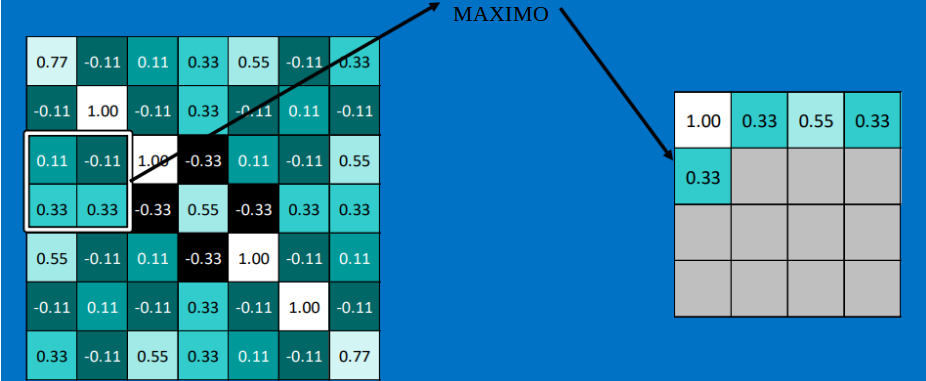
\includegraphics[width=0.75\textwidth]{images/marcoteorico/pool1}
		\end{center}
		\begin{center}
		\caption{\small{Operación MAX-pooling en capa de Agrupación}}
		\vskip -0.2cm  
		{\small{Fuente: \cite{Rohrer}}}
		\end{center}
		\vspace{-1.5em}
		\end{figure}

		Este proceso es aplicado para cada mapa de activación(salida de la capa de convolución). Análogamente con la capa de convolución, el resultado en esta capa es un conjunto de imágenes que muestran un versión agrupada de las imágenes de entrada.

		\begin{figure}[H]
		\begin{center}
		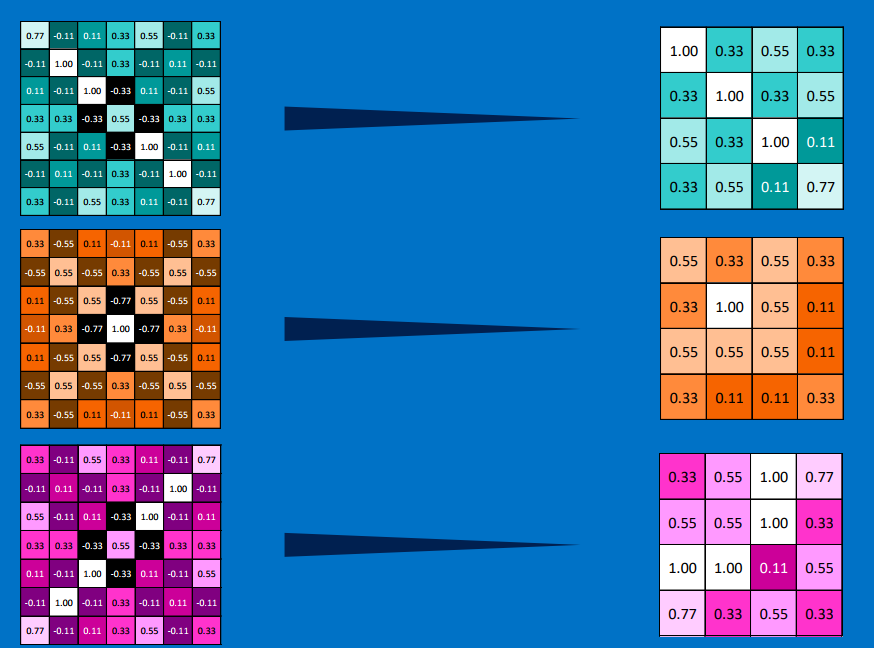
\includegraphics[width=0.7\textwidth]{images/marcoteorico/pool2}
		\end{center}
		\begin{center}
		\caption{\small{Resultado de Agrupación}}
		\vskip -0.2cm  
		{\small{Fuente: \cite{Rohrer}}}
		\end{center}
		\vspace{-1.5em}
		\end{figure}


		\noindent Esta capa pooling recibe como dato de entrada los parámetros:
		${W_{0}}\times{H_{0}}\times{D_{0}}$ \newline
		Y produce un dato de salida con los siguiente parámetros: ${W_{1}}\times{H_{1}}\times{D_{1}}$\newline
		
		% first column
		\begin{minipage}[t]{0.5\textwidth}
		En el que:
		\begin{center}
		 ${W_{1}} = \frac{{W_{0}} - F }{S} +1$ 
		\vskip 0.4cm 
		 ${H_{1}} = \frac{{H_{0}} - F }{S} +1$ 
		\vskip 0.4cm 
		 ${D_{1}} = {D_{0}}$ 
		 \end{center}
		\vskip 0.6cm 
		\end{minipage}
		%second column
		\begin{minipage}[t]{0.55\textwidth}
		Donde:
		\vskip 0.1cm 
		$W$ es el ancho (width) de la imagen, \vskip 0.4cm  
		$H$ es la altura (height) de la imagen,\vskip 0.4cm 
		$D$ es la profundidad (depth) de la imagen,\vskip 0.4cm 
		$F$ es la extensión espacial (spatial extent) del kernel,\vskip 0.4cm 
		$S$ es el paso (stride) del kernel,\vskip 0.4cm 
		\end{minipage}

		\begin{figure}[H]
		\begin{center}
		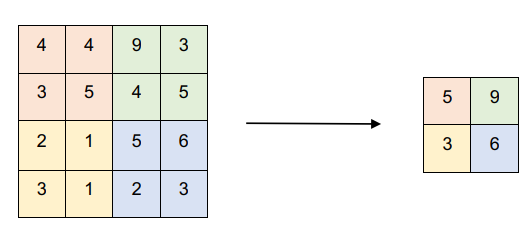
\includegraphics[width=0.5\textwidth]{images/marcoteorico/pool4}
		\end{center}
		\begin{center}
		\caption{\small{Max-pooling con filtro 2x2 y paso 2}}
		{\small{Fuente: Elaboración propia}}
		\end{center}
		\vspace{-1.5em}
		\end{figure}

	\subsection{Capa totalmente conectada (Fully-connected layer)}

		Esta capa por lo general aparece al final de la arquitectura y es similar al Perceptrón multicapa(MultilayerPerceptron -MLP), en el cual la neurona de salida se conecta a todas las neuronas de entrada y el peso de las conexiones son actualizadas usando el método de retropropagación.
		\vskip 0.4cm  
		Eventualmente, con un mapa de características lo suficientemente pequeño, el contenido se aplastará en un vector de una sola dimensión y será entrada para en un MLP totalmente conectado para su procesamiento.
		\vskip 0.4cm  
		Habiendo detallado que la función ReLU es la más utilizada en las capas anteriores, en esta última capa del modelo generalmente se utiliza una función de activación diferente, porque en esta capa se pretende que tenga una salida determinada. La {\bf función softmax} es muy popular cuando se hace la clasificación.
	


En resumen, una arquitecuta o modelo de red convolucional estará compuesto de varias capas y ejecutará las siguientas actividades:
\begin{figure}[H]
	\begin{center}
	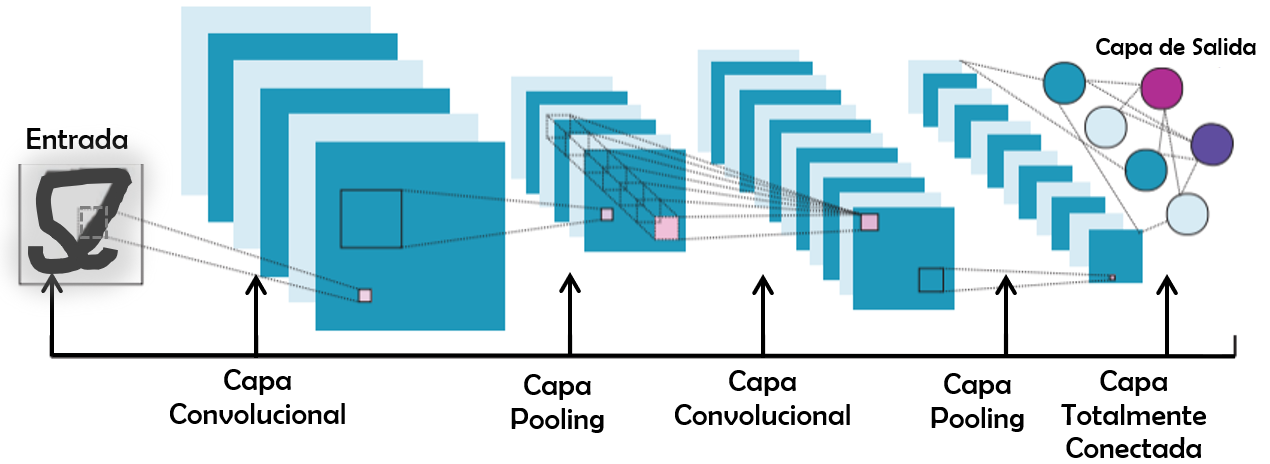
\includegraphics[width=0.8\textwidth]{images/marcoteorico/modelo}
	\end{center}
	\begin{center}
	\caption{\small{Modelo de red neuronal convolucional profunda}}
	{\small{Fuente: Elaboración propia}}
	\end{center}
	\vspace{-1.5em}
	\end{figure}

\begin{itemize}
	\item Se pasa una imagen de entrada a la primera capa convolucional. La salida complicada se obtiene como un mapa de activación. Los filtros aplicados en la capa de convolución extraen características relevantes de la imagen de entrada para pasar más lejos.\vspace{-0.5em}

	\item Cada filtro dará una característica diferente para ayudar a la predicción de clase correcta. En caso de que necesitemos retener el tamaño de la imagen, usamos el mismo relleno (padding cero), de lo contrario se usa el relleno válido ya que ayuda a reducir el número de características. \vspace{-0.5em}

	\item Las capas de agrupamiento se agregan para reducir aún más el número de parámetros.\vspace{-0.5em}

	\item Se agregan varias capas de convolución y agrupación antes de realizar la predicción. \vspace{-0.5em}

	\item A medida que profundizamos en la red, se extraen características más específicas en comparación con una red superficial donde las características extraídas son más genéricas. \vspace{-0.5em}

	\item La capa de salida en una CNN, como se mencionó anteriormente, es una capa totalmente conectada, donde la entrada de las otras capas se aplana y se envía para transformar la salida en el número de clases que desea la red. \vspace{-0.5em}

	\item La salida se genera a través de la capa de salida y se compara con la capa de salida para la generación de errores. Una función de pérdida se define en la capa de salida totalmente conectada para calcular el gradiente de error. \vspace{-0.5em}

	\item El error se retroproyecta para actualizar los valores de filtro (pesos) y sesgo(bias). \vspace{-0.5em}
	
	\item Finalmente, un ciclo de entrenamiento se completa en un solo pase hacia adelante y hacia atrás. Por lo que se tiene que repetir todo el proceso durante varios iteraciones para obtener mejores resultados.\vspace{-0.5em}

\end{itemize}
\newpage
\section{Entrenamiento y Validación}

	La red procesa los registros en los datos de entrenamiento uno a la vez, usando los pesos y las funciones en las capas ocultas, luego compara las salidas resultantes con las salidas deseadas. Los errores se propagan a través del sistema, lo que hace que el sistema ajuste los pesos y biases que serán procesados en la siguiente iteracion de entrenamiento. Este proceso ocurre una y otra vez para el mismo conjunto de datos, a medida que los pesos se ajustan(refianan)continuamente. Para realizar este proceso, existe una método de optimización muy popular denominado {\bf Descenso de gradiente}(Gradient Descent).

	\subsection{Descenso de Gradiente}

		Un gradiente mide cuánto cambia la salida de una función si se cambia un poco las entradas.

		En el caso del entrenamiento de una red neuronal, el gradiente simplemente mide el cambio en todos los pesos con respecto al cambio en el error. El gradiente se puede representar como la pendiente de una función. Cuanto más alto es el gradiente, más pronunciada es la pendiente y más rápido puede aprender un modelo. Pero si la pendiente es cero, el modelo deja de aprender. Dicho matemáticamente, un gradiente es una derivada parcial con respecto a sus entradas, \citep{gradient}.

		El descenso de gradiente es un algoritmo de optimización iterativa utilizado al entrenar un modelo de aprendizaje automático, basado en una función convexa, que ajusta sus parámetros iterativamente para minimizar la función de pérdida(error) hasta su mínimo local.\citep{gradient}

		\begin{figure}[H]
		\begin{center}
		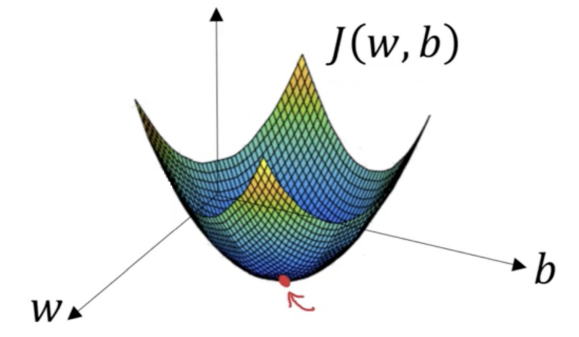
\includegraphics[width=0.8\textwidth,height=6.5cm]{images/desarrollo/entrenamiento/gradient}
		\end{center}
		\begin{center}
		\caption{\small{Establecimiento de la Tasa de Aprendizaje}}
		\vspace{-0.5em}
		{\small{\cite{gradientimg}}}
		\end{center}
		\vspace{-1.5em}
		\end{figure}
		

		La idea detrás del descenso de gradiente es disminuir de forma gradual, pero constante, el error de salida ajustando los pesos. Intuitivamente, se conoce que si un cambio en un peso aumentará (disminuirá) el error, entonces queremos disminuir (aumentar) ese peso. Matemáticamente, representa el cambio en el error dado un cambio de unidad en el peso:

		\begingroup\makeatletter\def\f@size{20.8}\check@mathfonts
		\begin{center}
		$ \frac{{\partial E}}{\partial w_{ij}}$
		\end{center}
		\begin{center}
		{\small{La derivada del error con respecto al peso}}
		\end{center}
		\endgroup
		
		Una vez que encontremos esta derivada, actualizamos el peso a través de lo siguiente:

		\begingroup\makeatletter\def\f@size{17.8}\check@mathfonts
		\begin{center}
		$  \triangle w_{ij} = -\eta\frac{{\partial E}}{\partial w_{ij}} $
		\end{center}
		\begin{center}
		{\small{Representación de la distancia por la dirección del cambio. $\eta$  es tasa de aprendizaje}}
		\end{center}
		\endgroup

		La tasa de Aprendizaje suele disminuir gradualmente durante las épocas de la fase de entrenamiento. Si actualizamos todos los pesos usando esta misma fórmula, esto equivale a moverse en la dirección de descenso más pronunciado a lo largo de la superficie de error, de ahí el nombre, descenso de gradiente.

		Se tienen diversos tipos, estos son:
		%con el objetivo principal de optimizar la funcion de error o pérdida de la red y por consecuente garantizar que el modelo neuronal pueda generalizar las clasificaciones a realizar. 
		\subsubsection{Gradiente Descendiente por Lotes(Batch Gradient Descent)}
		
			Calcula el error para cada ejemplo dentro del conjunto de datos de entrenamiento, pero el modelo se actualiza solo después de que se hayan evaluado todos los ejemplos de entrenamiento Todo este proceso es como un ciclo y se denomina época de entrenamiento.

		\subsubsection{Gradiente Descendiente Estocástico(Stochastic Gradient Descent-SGD)}

			Por el contrario, hace esto para cada ejemplo de entrenamiento dentro del conjunto de datos. Esto significa que actualiza los parámetros para cada ejemplo de entrenamiento, uno por uno. Esto puede hacer que el SGD sea más rápido que el Descenso de gradiente por lotes, dependiendo del problema. Una ventaja es que las actualizaciones frecuentes nos permiten tener una tasa de mejora bastante detallada. El hecho es que las actualizaciones frecuentes son más costosas desde el punto de vista computacional que el enfoque del BGD y La frecuencia de esas actualizaciones también puede generar gradientes ruidosos, lo que puede hacer que la tasa de error salte, en lugar de disminuir lentamente.

			El MOMENTUM es otro argumento en el optimizador SGD que podríamos ajustar para obtener una convergencia más rápida. Ayuda al vector de parámetros a aumentar la velocidad en cualquier dirección con un descenso constante del gradiente para evitar oscilaciones. Una elección típica de momento es entre 0.5 a 0.9.

		\subsubsection{Mini-batch Gradient Descent}

			Es el método de más usado, ya que es una combinación de los conceptos de SGD y Batch Gradient Descent. Simplemente divide el conjunto de datos de entrenamiento en pequeños lotes y realiza una actualización para cada uno de estos lotes. Por lo tanto, crea un equilibrio entre la robustez del descenso del gradiente estocástico y la eficiencia del descenso del gradiente discontinuo.





	\subsection{Tasa de Aprendizaje (Learning Rate)}
		Uno de los hiperparámetros clave durante el entrenamiento deuna red neuronal es la velocidad/tasa de aprendizaje para el descenso del gradiente.
		Este parámetro puede entenderse como el tamaño del paso en la optimización para minimizar la función de pérdida de la red, es decir, es un parámetro que determina cuánto influye un paso de actualización en el valor actual de los pesos, por ejemplo, el tamaño del paso en el que el gradiente cae en la dirección máxima de la pendiente, \citep {AdamImg}.

		\begin{figure}[H]
		%\begin{center}
		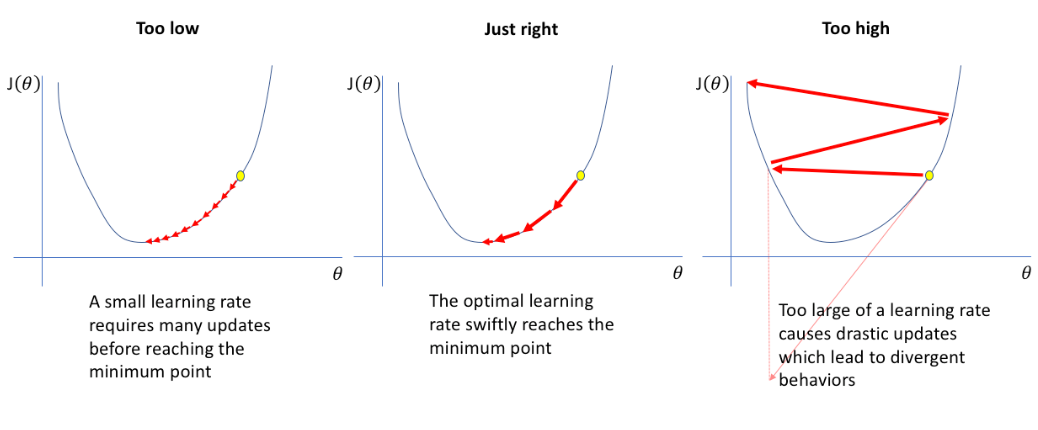
\includegraphics[width=1\textwidth]{images/desarrollo/entrenamiento/LR}
		%\end{center}
		\begin{center}
		\caption{\small{Establecimiento de la Tasa de Aprendizaje}}
		\vspace{-0.5em}
		{\small{\cite{AdamImg}}}
		\end{center}
		\vspace{-1.5em}
		\end{figure}

		Cuando la tasa de aprendizaje es demasiado pequeña, es necesario realizar muchas iteraciones de aprendizaje; pero cuando la tasa de aprendizaje es demasiado grande, el resultado se moverá hacia adelante y hacia atrás en ambos sentidos de los valores extremos(oscila), y no se podrá lograr la solución óptima como puede ser observado en la figura 2.25.

		Debido a esto es que al entrenar redes neuronales profundas, a menudo es útil reducir la tasa de aprendizaje a medida que avanza el entrenamiento y no mantenerlo constante y asi evitar la divergencia(Punto apartir del cual la pérdida ya no se reduce y en lugar de eso comienza a incrementarse).


		\begin{figure}[H]
		%\begin{center}
		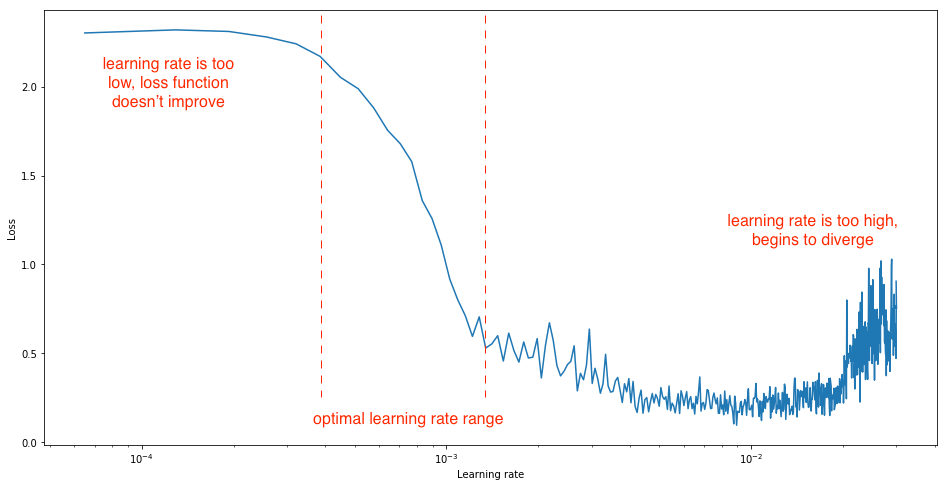
\includegraphics[width=1\textwidth]{images/desarrollo/entrenamiento/lr_finder}
		%\end{center}
		\begin{center}
		\caption{\small{Problemas con la Tasa de Aprendizaje}}
		{\small{\cite{AdamImg}}}
		\end{center}
		\vspace{-1.5em}
		\end{figure}

		Reduciendo lentamente la tasa de aprendizaje a lo largo del tiempo ayuda a acelerar el aprendizaje. Esto es lo que se conoce como tasa de decaimiento de aprendizaje{\bf(learning rate decay)}.
			\begin{figure}[H]
				\begin{center}
				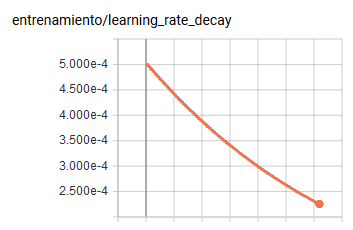
\includegraphics[width=0.6\textwidth,height=5.5cm]{images/desarrollo/entrenamiento/LR_decay} 
				\end{center}
				\begin{center}
				\caption{\small{Ejemplo de Tasa de decaimiento de aprendizaje por época  }}
				\vspace{-0.5em}
				{\small{\fontsize{10}{16.8}\selectfont {Fuente: Elaboración propia}}}
				\end{center}
				\vspace{-1.5em}
			\end{figure}
		Sin embargo, el optimizador Gradient Descent(en cualquiera de sus tipos) con una tasa de decaimiento de aprendizaje, no es usado a menudo para entrenar redes neuronales profundas ya que genera un desafío el determinar los hiperparámetros que deben definirse de antemano y dependen en gran medida del tipo de modelo y problema. Además de que la misma tasa de aprendizaje se aplica a todas las actualizaciones de los parámetros. Por lo que opta en usar optimizadores más avanzados que tienen una tasa de convergencia más rápida y adaptable a diversas situaciones. Proporcionan una alternativa a los clásicos y son conocidos como optimizadores de descenso de gradiente de segundo orden; algunos de ellos son: Adagrad, Adadelta, RMSprop, Adam. 

		%AdaGrad or adaptive gradient allows the learning rate to adapt based on parameters. It performs larger updates for infrequent parameters and smaller updates for frequent one. Because of this it is well suited for sparse data (NLP or image recognition). Another advantage is that it basically illiminates the need to tune the learning rate. Each parameter has its own learning rate and due to the peculiarities of the algorithm the learning rate is monotonically decreasing. This causes the biggest problem: at some point of time the learning rate is so small that the system stops learning.AdaDelta resolves the problem of monotonically decreasing learning rate in AdaGrad. In AdaGrad the learning rate was calculated approximately as one divided by the sum of square roots. At each stage you add another square root to the sum, which causes denominator to constantly decrease. In AdaDelta instead of summing all past square roots it uses sliding window which allows the sum to decrease. RMSprop is very similar to AdaDelta. Adam or adaptive momentum is an algorithm similar to AdaDelta. But in addition to storing learning rates for each of the parameters it also stores momentum changes for each of them separately

		En esta investigación se usaran los métodos de Descenso de Gradiente Mini-batch y optimzador Adam, conjuntamente con una tasa de decaimiento de aprendizaje.

	\subsection{Optimizador ADAM}
	
		El método calcula las tasas de aprendizaje individuales de manera adaptativa para diferentes parámetros a partir de las estimaciones de los primeros y segundos momentos de los gradientes; el nombre Adam deriva de Estimación del Momento Adaptativo \citep {Adam},

		Permite que la tasa de aprendizaje se adapte según los parámetros. Realiza actualizaciones más grandes para parámetros infrecuentes y actualizaciones más pequeñas para los frecuentes. Debido a esto, es adecuado para datos dispersos (NLP o reconocimiento de imágenes). Otra ventaja es que básicamente simplifica la necesidad de ajustar la tasa de aprendizaje. Cada parámetro tiene su propia tasa de aprendizaje, sin embargo, la tasa de aprendizaje no disminuye monótonamente. Además de almacenar las tasas de aprendizaje para cada uno de los parámetros, también almacena los cambios de momento para cada uno de ellos por separado .

	\subsection{Validación Cruzada}
	
		%Cross-entropy loss, or log loss, measures the performance of a classification model whose output is a probability value between 0 and 1. Cross-entropy loss increases as the predicted probability diverges from the actual label. So predicting a probability of .012 when the actual observation label is 1 would be bad and result in a high loss value. A perfect model would have a log loss of 0.

		Para el entrenamiento, el conjunto de datos se divide en un subconjunto de entrenamiento y otro para validación. En esta investigación se dividirá el 75\% para entrenamiento y 75\% para validación, {\citep {Elkan12evaluatingclassifiers}}. La división en subgrupos de entrenamiento y validación generalmente se realiza de manera aleatoria, para garantizar que ambos subconjuntos sean muestras aleatorias de la misma distribución. Puede ser razonable realizar un muestreo estratificado, lo que significa asegurar que cada clase esté presente en la misma proporción en los subconjuntos de entrenamiento y prueba. En esta investigación se trabajará con 2 tipos de muestreos (balanceado/estratificado y no balanceado)

		Se utiliza el subconjunto de validación para evaluar el desempeño de diferentes arquitecturas del modelo (diferentes topologías), para luego escoger una de ellas. Este subconjunto(de validación) se usa para verificar si el error está dentro de algún rango y no se usa directamente para ajustar los pesos, por el contrario \textbf{se usa para indicar el número óptimo de neuronas ocultas o determina el punto de parada para el entrenamiento}.  Por lo tanto, el modelo es entrenado sobre el conjunto de entrenamiento completo y la capacidad de generalización es medida en el conjunto de validación. 

		La validación cruzada o cross-validation es una técnica utilizada para evaluar los esultados de un análisis estadístico y garantizar que son independientes de la partición entre datos de entrenamiento y validación, \citep{moore2001cross}. En problemas de clasificación, debido a que los datos se dividen en clases finitas, es natural pensar que la categoría al cual pertenece cierto resultado se dará a través de probabilidades. En probabilidad, la entropía cruzada es la distancia entre las dos distribuciones de probabilidad y se usa generalmente como la función de pérdida. Es por ello que el resultado de la validación cruzada representa la pérdida de la entropía del conjunto de datos. La entropía se suele utilizar en la teoría de la información para medir la pureza o impureza de un conjunto determinado. La pregunta a la que responde es: ¿Cuánto diferente esos elementos son entre sí?.  

			\begingroup\makeatletter\def\f@size{17.8}\check@mathfonts
			\begin{center}
			$H(p,q) = -\sum_{\forall x} p(x) log(q(x))$
			\end{center}
			\begin{center}
			{\small{Fórmula de entropía cruzada con dos distribuciones sobre la variable discreta $x$, donde $q(x)$ es la estimación para la clasificación verdadera $p(x)$}}
			\end{center}
			\endgroup		

		Para una red neuronal, normalmente verá la ecuación escrita en una forma donde $y$ es el vector de verdad y la variable $\hat{y}$ (o algún otro valor tomado directamente de la última salida de la capa) es la estimación, y se vería así para un solo ejemplo:
			
			\begingroup\makeatletter\def\f@size{17.8}\check@mathfonts
			\begin{center}
			$L = - \mathbf{y} \cdot log(\mathbf{\hat{y}})$
			\end{center}
			%\begin{center}
			%{\small{El valor es independiente de cómo la probabilidad restante se divide entre clases incorrectas}}
			%\end{center}
			\endgroup		
		
		A menudo esta ecuación es promediada sobre todos los ejemplos como una función de costo. No siempre se cumple estrictamente en las descripciones, pero generalmente una función de pérdida es de nivel inferior y describe cómo una sola instancia o componente determina un valor de error, mientras que una función de costo es de nivel superior y describe cómo se evalúa un sistema completo para la optimización. Una función de costo basada en pérdida de clasificación multiclase para un conjunto de datos de tamaño N podría verse así:
		
			\begingroup\makeatletter\def\f@size{17.8}\check@mathfonts
			\begin{center}
			$J = - \frac{1}{N}(\sum_{i=1}^{N} \mathbf{y_i} \cdot log(\mathbf{\hat{y}_i}))$
			\end{center}
			\begin{center}
			{\small{Cálculo de la función de costo en la validación de clasificación de datos}}
			\end{center}
			\endgroup		
	

		Es por ello que la la función de costo/pérdida dada por la validacion cruzada ayuda para decidir cuándo se debe terminar el entrenamiento de una red.\citep{AulaMLP}. Usualmente se utiliza el error cuadrático medio como función de pérdida para medir el rendimiento de un modelo de regresion. Sin embargo, en casos de clasificación, la función de costo de pérdida a través del cálculo de la entropía cruzada es preferible, ya que tiende a no causar saturación de las neuronas de salida, convirtiendo el aprendizaje más rápido,\citep{AulaDNN}.

		La pérdida de entropía cruzada aumenta a medida que la probabilidad prevista diverge de la clasificación real. Por lo tanto, un modelo casi perfecto tendría una pérdida de entropía cercana a cero, \citep{crossMSE}.
		


	\subsection{Función Softmax}
		Conocida tambien como función exponencial normalizada, es la funcion de activación utilizada en la última capa de una red neuronal. La salida de una red neuronal completamente conectada no es una distribución de probabilidad, sin embargo, el uso de esta función ayuda a obternela. Por lo que esta función permitirá estimar la probabilidad de que la imagen de entrada pertenezca a cada una de las clases al realizar una normalización con el objetivo que el valor de cada neurona esté limitado entre cero y uno y así permitir que el resultado de las neuronas de salida sumen a uno. 

			\begingroup\makeatletter\def\f@size{17.8}\check@mathfonts
			\begin{center}
			${\displaystyle P(y=j\mid \mathbf {x} )={\frac {e^{\mathbf {x} ^{\mathsf {T}}\mathbf {w} _{j}}}{\sum _{k=1}^{K}e^{\mathbf {x} ^{\mathsf {T}}\mathbf {w} _{k}}}}}$
			\end{center}
			\begin{center}
			{\small{Función Softmax}}
			\end{center}
			\endgroup
			
		Esto se puede ver como la composición de K funciones lineales ${x} \mapsto \mathbf {x} ^{\mathsf {T}}\mathbf {w} _{1},\ldots ,\mathbf {x} \mapsto \mathbf {x} ^{\mathsf {T}}\mathbf {w} _{K}$, donde ${\mathbf {x} ^{\mathsf {T}}\mathbf {w}}$ denota el producto interno de $x$(entrada) y $w$(peso).	La operación es equivalente a aplicar un operador lineal definido por $ w $ a vectores $ x $, transformando así la entrada original, probablemente altamente dimensional(reales arbitrarios), en vectores K-dimensional de valores reales en el rango [0, 1] que suman 1. \citep{Bishop}. 

		Esta función permite que al estar normalizadas las salidas de la segunda capa totalmente conectada, pueda ser aplicada la validación cruzada y conocer la pérdida de entropía.

	
	\subsection{Método de Regularización L2}
		En la regularización, lo que se hace normalmente es mantener el mismo número de funciones, pero se reduce la magnitud de los coeficientes.

		

		El método de Regularización L2 o también conocido como Regresión Lasso (Lasso Regression - Least Absolute Shrinkage and Selection Operator), trata de agregar un término adicional(lambda) a la función de pérdida, la cual penaliza parametrizaciones con pesos más elevados,\citep{AulaMLP}, es decir, reduce el coeficiente de la función menos importante a cero, eliminando así algunas características. Por lo tanto, esto funciona bien para la selección de funciones en caso de que tengamos una gran cantidad de funciones.

		Si $L(\theta, D)$ es la función de pérdida (en esta investigación - entropía cruzada), $\theta$ es el conjunto de parámetros libres y $D$ es un ejemplo de entrenamiento, entonces a la función de pérdida regularizada será:

			\begingroup\makeatletter\def\f@size{17.8}\check@mathfonts
			\begin{center}
			$E(\theta,D) =L(\theta,D) +\lambda R(\theta)$
			\end{center}
			\endgroup
		

		Donde $R(\theta)$ caracteriza la complejidad del modelo y $\lambda$ representa la proporción de la pérdida total del modelo, generalmente $\lambda$ estará cerca de 0 porque si $\lambda$ es demasiado grande, conducirá a un ajuste insuficiente(underfitting). Por otro lado, para evitar el exceso de ajuste(overfitting) cuando se tiene una gran cantidad de características en su conjunto de datos, no optimizamos directamente $L(\theta,D)$ (cross entropy), sino que optimizamos $L(\theta,D) +\lambda R(\theta)$

		Se usará una constante {\bf lambda($\lambda$) = 0.0001}, por defecto. La regularización de pérdida L2 solo debe incluir los pesos de las capas totalmente conectadas, y normalmente no incluye a los bias(sesgos). La intuición detrás de esto es que el bias contribuye al overfitting(sobreajuste), y no estaría agregando ningún nuevo grado de libertad al modelo.



%============================================================================================================%============================================================================================================%============================================================================================================%============================================================================================================


\section{Método de la investigación}

\subsection{ Tipo de investigación}
	De acuerdo al fin que se persigue es una investigación de tipo tecnológica y de acuerdo al diseño es una investigación experimental de tipo cuantitativa donde se analizará el rendimiento del modelo algorítmico.

\subsection{Variables de la Investigación}
		
		\subsubsection{Variable Dependiente}
		\indent Reconocimiento automático de señales de tránsito vehicular
		\subsubsection {Variable Independiente}
		\indent Modelo basado en el aprendizaje profundo de redes neuronales convolucionales	
		
\subsection{Indicadores}
		\renewcommand{\baselinestretch}{2}
		Los indicadores nos permiten realizar mediciones y a su vez determinan la validez de la hipótesis planteada en la presente investigación. El desempeño de la clasificación se puede verificar con los siguinetes cinco indicadores: 
		\begin{table}[H]
		\centering
		\caption{\small{Indicadores para la investigación}}
		\begin{tabular}{|>{\small}c|>{\small}c|>{\small}c|}
		\hline
		{\ul \textbf{Indicador}} & {\ul \textbf{Descripcion}} & {\ul \textbf{Instrumento}} \\ \hline
		\multirow{2}{*}{\begin{tabular}[c]{@{}c@{}}Tasa de Verdaderos Positivos\\ (Efectividad - Sensibilidad)\end{tabular}} & \multirow{2}{*}{$ \frac{Verdaderos\,Positivos}{{Verdaderos\,Positivos}+{Falsos\,Negativos}}$} & \multirow{2}{*}{\begin{tabular}[c]{@{}c@{}}Modelo de\\ Reconocimiento\end{tabular}} \\
		 &  &  \\ \hline
		\multirow{2}{*}{\begin{tabular}[c]{@{}c@{}}Tasa de Verdaderos Negativos \\ (Especificidad)\end{tabular}} & \multirow{2}{*}{$ \frac{Verdaderos\,Negativos}{{Verdaderos\,Negativos}+{Falsos\,Positivos}}$} & \multirow{2}{*}{\begin{tabular}[c]{@{}c@{}}Modelo de\\ Reconocimiento\end{tabular}} \\
		 &  &  \\ \hline
		 \multirow{2}{*}{\begin{tabular}[c]{@{}c@{}}Valor Predictivo Positivo \\ (Precisión)\end{tabular}} & \multirow{2}{*}{$ \frac{Verdaderos\,Positivos}{{Verdaderos\,Positivos}+{Falsos\,Positivos}}$} & \multirow{2}{*}{\begin{tabular}[c]{@{}c@{}}Modelo de\\ Reconocimiento\end{tabular}} \\
		 &  &  \\ \hline
		 \multirow{2}{*}{\begin{tabular}[c]{@{}c@{}}Curvas PR \\ (Precision - Recall)\end{tabular}} & \multirow{2}{*}{Relación entre Efectividad(Recall) y Precision} & \multirow{2}{*}{\begin{tabular}[c]{@{}c@{}}Modelo de\\ Reconocimiento\end{tabular}} \\
		 &  &  \\ \hline
		%\multirow{2}{*}{\begin{tabular}[c]{@{}c@{}}Tiempo de\\ Procesamiento\end{tabular}} & \multirow{2}{*}{$S= \frac{\sum_{i=1}^{Total} tiempo_{i}}{Total\,de\,muestras}$} & \multirow{2}{*}{\begin{tabular}[c]{@{}c@{}}Cronometro\\ Computacional\end{tabular}} \\
		\multirow{2}{*}{\begin{tabular}[c]{@{}c@{}}Curvas ROC \\ (Receiver Operating Characteristic)\end{tabular}} & \multirow{2}{*}{Relación entre Efectividad y Especificidad} & \multirow{2}{*}{\begin{tabular}[c]{@{}c@{}}Modelo de\\ Reconocimiento\end{tabular}} \\
		 &  &  \\ \hline
		\multirow{2}{*}{\begin{tabular}[c]{@{}c@{}}Tasa de Acuracia \\ (Exactitud)\end{tabular}} & \multirow{2}{*}{$ \frac{Verdaderos\,Positivos+Verdaderos\,Negativos}{Total\,de\,Imagenes}$} & \multirow{2}{*}{\begin{tabular}[c]{@{}c@{}}Modelo de\\ Reconocimiento\end{tabular}} \\
		 &  &  \\ \hline		 
		\end{tabular}
		\vspace{-1.0em}
		\end{table}

	\newpage
\subsection{Recolección de Datos para la Construcción del Modelo}
		%\renewcommand{\baselinestretch}{1.2}
		\subsubsection{Técnica de Recolección}
		\begin{enumerate}		
			\item[]   {Revisión de la literatura(análisis de documentos)}
		\end{enumerate}

		\subsubsection{Población}
		\begin{enumerate}		
			\item[] Existen diversas arquitecturas de redes neuronales convolucionales usadas para propósitos específicos. La idea principal es que al principio la arquitectura de la red neuronal toma como entrada una imagen y su especificación de dimensiones en 3 valores(largo, ancho y profundidad). Capas convolucionales y capas de activación(optimización) se apilan juntas y luego son seguidas por capas de agrupamientos. Esta estructura se usa comúnmente y se repite hasta que la entrada (imagen) se fusiona espacialmente a un tamaño pequeño. Después de eso, se envía a capas completamente conectadas y la salida de la última capa completamente conectada, que está al final de la arquitectura, produce los puntajes de clase de la imagen de entrada.
		\end{enumerate}
		
	
		\subsubsection{Muestra}
		\begin{enumerate}		
		\item[] Para el proceso de diseño e implementación de arquitecturas a elaborar se tomarán en cuenta dos modelos mundialmente conocidos e importantes:
		\end{enumerate}
				
		\begin{enumerate}
		\item[] {\bf \underline {Arquitectura AlexNet }}\newline
			Esta arquitectura hizo que las Redes Convolucionales fueran populares en el campo de Visión por Computadora. AlexNet fue desarrollado por \citep{Krizhevsky2012}. La entrada consiste en una imagen de 224x224 pixeles en formato RGB (3 canales). La arquitectura consta de 8 capas, las primeras cinco capas son convolucionales y el resto son capas totalmente conectadas. La primera y segunda capa convolucional son seguidas por capas de normalización de respuesta local, luego estas capas de normalización de respuesta son seguidas por capas de agrupación máxima. La salida de cada capa convolucional y cada capa completamente conectada se activa a través de  una función no linear conocida como RELU. Similar a LenNet-5\citep{LeCun} pero más grande, teniendo aproximadamente 60 millones de parámetros.
		\end{enumerate}

		\begin{enumerate}
		\item[] {\bf \underline {Arquitectura Inception}}\newline
			Es una arquitectura de red neuronal convolucional profunda, creada por un grupo de investigación de Google que fue responsable de establecer el nuevo estado del arte de la técnica para la clasificación y detección en la competencia de reconocimiento visual a gran escala ImageNet 2014(ILSVRC14). 
			\vskip 0.1cm
			El principal sello distintivo de esta arquitectura es la utilización mejorada de los recursos informáticos dentro de la red. Esto fue logrado por un cuidadoso que permite aumentar la profundidad y el ancho de la red mientras se manteniene el costo computacional constante. Para optimizar la calidad, las decisiones para elaborar la arquitectura se basaron en el principio Hebbiano y la intuición de procesamiento a escala múltiple. Una encarnación particular utilizada en la competencia ILSVRC14 es llamada GoogLeNet, una red de 22 capas de profundidad, cuya calidad se evalúa en el contexto de reconocimiento y detección, \citep{Inception}.
		\end{enumerate}
		%====================================================================================
		% subsection Recolección de Datos para la Construcción del Modelo (end)

	\subsection{Recolección de Datos para el Entrenamiento y Evaluación del Modelo}
		
		\subsubsection{Técnica de Recolección}
		\begin{enumerate}		
			\item[]  Revisión de la literatura(análisis de documentos) y captura de imágenes del Perú a través de la aplicación Google Maps
		\end{enumerate}

		\subsubsection{Población} 
		\begin{enumerate}
		\item[]				
		{\bf *) Área:} Imágenes de Señales de Seguridad Vial.\vskip 0.1cm
		{\bf *) Categoría:} Tránsito Vehicular Vertical.\vskip 0.1cm
		{\bf *) Subcategoría:} Señales reguladoras, preventivas e informativas.\vskip 0.1cm
		\end{enumerate}

		\begin{enumerate}		
			\item[]  La población es infinita para esta investigación, debido al número infinito de formas distintas en que una señal de tránsito puede ser capturada.Se tomaran en cuenta imágenes donde se muestren señales de tránsito vehicular del tipo vertical en sus 3 subcategorias.
		\end{enumerate}

		\subsubsection{Muestra} 
		\begin{enumerate}		
			\item[]	Existe una colección(dataset) que se ajusta a las características de nuestra población y será usada para conseguir el objetivo de la investigación, principalmente porque cuenta con abundantes imágenes lo que conforma una muestra representativa y necesaria para hacer generalizaciones. 
		\end{enumerate}

		\begin{enumerate}
			\item[]  {\bf \underline {Señales de Tránsito de Alemania}}\newline
			Conjunto de datos creados a partir de aproximadamente 10 horas de video grabados durante el día mientras se conducía en diferentes tipos de carreteras en Alemania. De las secuencias del video fueron extraídas imágenes de señales de tránsito en formato RGB cuyas dimensiones varían entre 15x15 y 250x250 pixeles. En esta colección se obtuvieron un total de 39209 imágenes distribuidas en 43 clases.  \citep{Stallkamp-IJCNN-2011} 
		\end{enumerate}

		%\item[B)] {\bf Señales de Tránsito de Bélgica} \citep{Timofte-MVA-2011} \newline
		%	Conjunto de datos creados con a la captura simultánea de imágenes durante el día realizada por 8 cámaras mientras se conducía aproximadamente a 35Km/h, con el objetivo de obtener una localización 3D y un refinamiento simultáneo. Las señales de tránsito fueron capturados a una distancia de menos de 50 metros y almacenadas en formato PPM cuyas dimensiones varían entre 25x30 y 260x250 pixeles. En esta colección se obtuvieron un total de 7125 imágenes distribuidas en 62 clases.
		
		
		\begin{enumerate}
			\item[]  {\bf \underline {Señales de Tránsito de Perú}}\newline
			Conjunto de aproximadamente 614 imágenes originalmente tomadas de la aplicación Google Maps agrupadas en 7 categorías. Dado que la población de imágenes es infinita, se optó por usar un muestreo aleatorio simple para poblaciones desconocidas con un nivel de confianza del 95\% y un error de muestreo del 4\%.
		
			\vskip 0.4cm
			\begingroup\makeatletter\def\f@size{17.8}\check@mathfonts
			\begin{center}
				${\bf n} ={\bf \frac{z^2pq}{e^2}}$
			\end{center}
			\endgroup
		
			En el que:\vskip 0.1cm
			\begin{itemize}
				\item $n$ = tamaño de muestra
				\item $z$ = Coeficiente de confiabilidad 95\% al que corresponde (1.96)
				\item $pq$ = Varianza de la población, ponemos la varianza mayor posible porque a mayor varianza hará falta una muestra mayor(0.25)
				\item $e$ = Error muestral(0.04)
			\end{itemize}
		\end{enumerate}
		%====================================================================================
		% subsection Recolección de Datos para el Entrenamiento y Evaluación del Modelo (end)

\subsection{Etapas de la investigación} 
	El desarrollo de la investigación comprenderá las siguientes etapas de trabajo a saber:

		\begin{enumerate}

		\item[a)]	Investigación bibliográfica de los diferentes temas necesarios para la elaboración de la investigación, tales como dispositivos de control de tránsito, vehículos autónomos, sistemas avanzados de asistencia al conductor, aprendizaje profundo (deep learning), procesamiento de imágenes, entre otros.
		
		\item[b)]	Búsqueda de los principales casos de éxito en el reconocimiento de señales de tránsito a tráves de trabajos de investigación en el Perú como tambíen en otros países.

		\item[c)]	Recolección de imágenes de señales de tránsito vehicular que se utilizarán en el desarrollo de la investigación.

		\item[d)]	Análisis e implementación de diversas técnicas de procesamiento de imágenes que serán aplicadas al dataset recolectado con la finalidad de contribuir en el diseño inicial del modelo modelo convolucional.

		\item[e)]	Puesto a que las redes neuronales son heurísticas por naturaleza (requieren un constante ajuste de híper-parámetros para obtener un óptimo resultado), se realizarán diferentes diseños de arquitecturas de modelos convolucionales y se escogerá el modelo que otorge los mejores resultados.
		
		\item[f)]	Para el análisis de resultados, además de los indicadores conocidos com tasa de sensibilidad, especificidad, precisión, se pretende usar una Matriz de confusión. A través de esta matriz se pueden conocer valores estadísticos del espacio ROC(Receiver Operating Characteristic), métrica usada para evaluar la calidad del modelo reconocedor.
		
		\end{enumerate}

		\subsubsection{Metodología para el diseño del Modelo}

			Se utilizará la metodología propuesta por Tammy Noergard (T. Noergaard, 2005) , la cual toma mucha de las claves de las metodologías conocidas como Rational Unified Process (RUP), Attribute Driven Desing (ADD), Object Oriented Process (OOP) y el Model Driven Architecture (MDA), pero las simplifica. La siguiente figura muestra las diferentes fases de la metodología.
			
			\begin{figure}[H]
			\begin{center}
			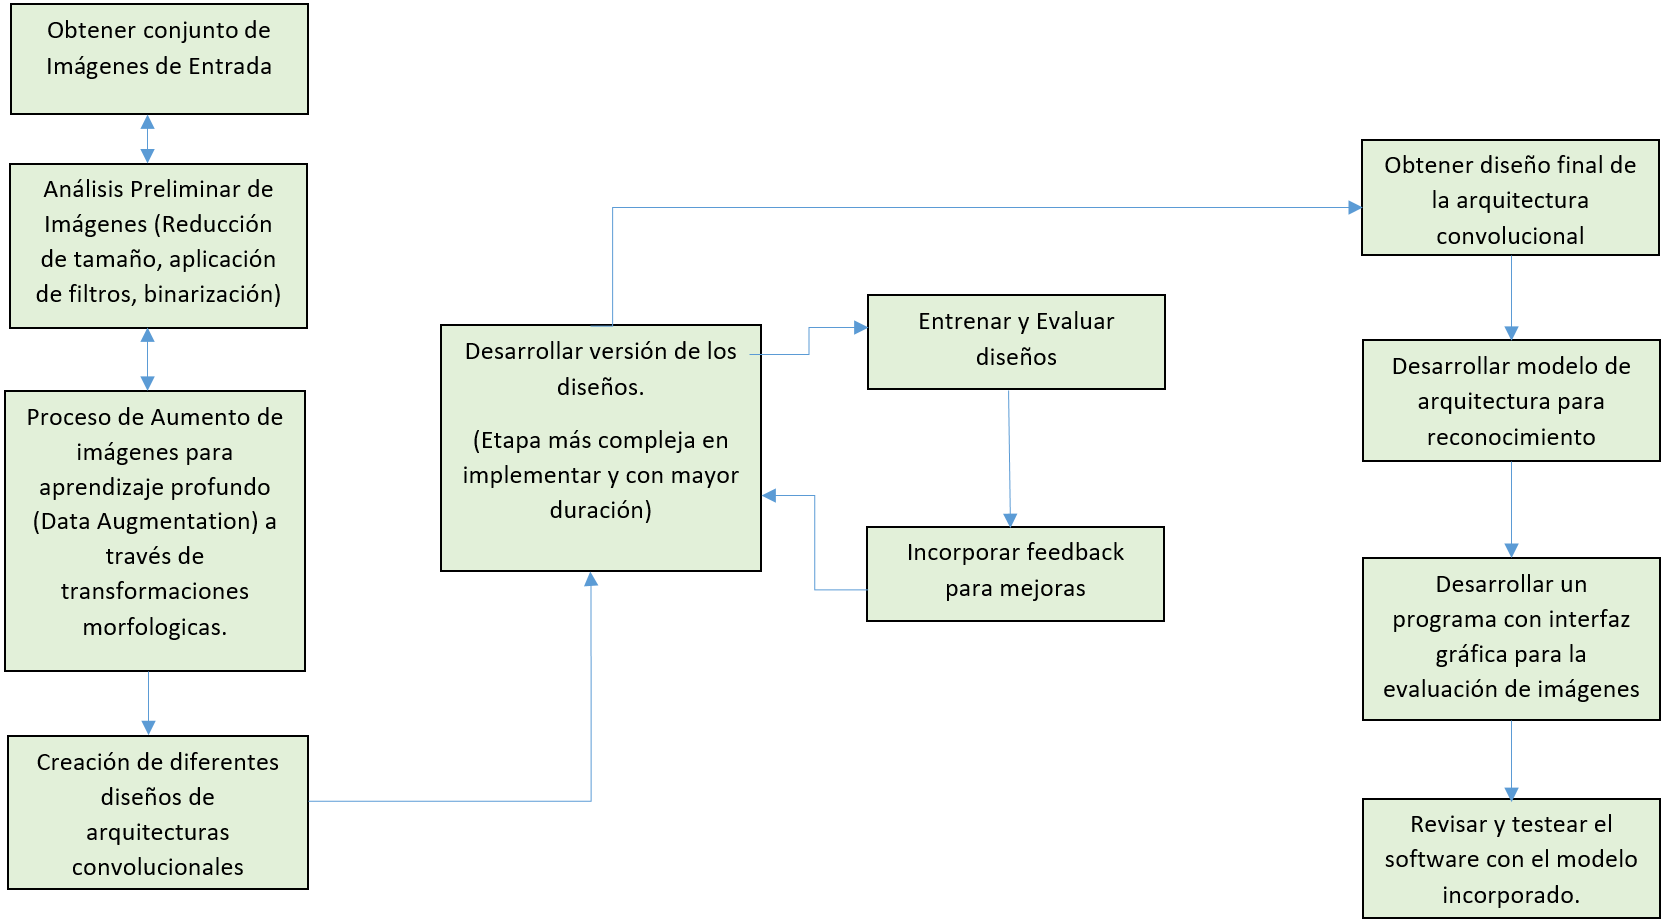
\includegraphics[width=0.9\textwidth]{images/intro/disenho}
			\end{center}
			\begin{center}
			\vskip 0.6cm	
			\caption{\small{Diseño del Modelo del Ciclo de Vida del Desarrollo}}
			{\small{Fuente: Elaboración propia}}
			\end{center}
			\vspace{-1.5em}
			\end{figure}


% subsection Etapas de la investigación (end)



	    % capitulo de marco teorico
	%!TEX root = origin.TEX
\chapter{Materiales y Técnicas}
\pagenumbering{arabic}
\setcounter{page}{53}
\renewcommand{\baselinestretch}{1.2} %doble espacio paratodo el texto

\section{ Tipo de investigación}
	De acuerdo al fin que se persigue es una investigación de tipo tecnológica y de acuerdo al diseño es una investigación experimental de tipo cuantitativa donde se analizará el rendimiento del modelo algorítmico.

\section{Variables de la Investigación}
		
		\subsection{Variable Dependiente}
		\indent Reconocimiento automático de señales de tránsito vehicular
		\subsection {Variable Independiente}
		\indent Modelo basado en el aprendizaje profundo de redes neuronales convolucionales	
		
	\section{Indicadores}
		\renewcommand{\baselinestretch}{2}
		Los indicadores nos permiten realizar mediciones y a su vez determinan la validez de la hipótesis planteada en la presente investigación. El desempeño de la clasificación se puede verificar con los siguinetes cinco indicadores: 
		\begin{table}[H]
		\centering
		\caption{\small{Indicadores para la investigación}}
		\begin{tabular}{|>{\small}c|>{\small}c|>{\small}c|}
		\hline
		{\ul \textbf{Indicador}} & {\ul \textbf{Descripcion}} & {\ul \textbf{Instrumento}} \\ \hline
		\multirow{2}{*}{\begin{tabular}[c]{@{}c@{}}Tasa de Verdaderos Positivos\\ (Efectividad - Sensibilidad)\end{tabular}} & \multirow{2}{*}{$ \frac{Verdaderos\,Positivos}{{Verdaderos\,Positivos}+{Falsos\,Negativos}}$} & \multirow{2}{*}{\begin{tabular}[c]{@{}c@{}}Modelo de\\ Reconocimiento\end{tabular}} \\
		 &  &  \\ \hline
		\multirow{2}{*}{\begin{tabular}[c]{@{}c@{}}Tasa de Verdaderos Negativos \\ (Especificidad)\end{tabular}} & \multirow{2}{*}{$ \frac{Verdaderos\,Negativos}{{Verdaderos\,Negativos}+{Falsos\,Positivos}}$} & \multirow{2}{*}{\begin{tabular}[c]{@{}c@{}}Modelo de\\ Reconocimiento\end{tabular}} \\
		 &  &  \\ \hline
		 \multirow{2}{*}{\begin{tabular}[c]{@{}c@{}}Valor Predictivo Positivo \\ (Precisión)\end{tabular}} & \multirow{2}{*}{$ \frac{Verdaderos\,Positivos}{{Verdaderos\,Positivos}+{Falsos\,Positivos}}$} & \multirow{2}{*}{\begin{tabular}[c]{@{}c@{}}Modelo de\\ Reconocimiento\end{tabular}} \\
		 &  &  \\ \hline
		 \multirow{2}{*}{\begin{tabular}[c]{@{}c@{}}Curvas PR \\ (Precision - Recall)\end{tabular}} & \multirow{2}{*}{Relación entre Efectividad(Recall) y Precision} & \multirow{2}{*}{\begin{tabular}[c]{@{}c@{}}Modelo de\\ Reconocimiento\end{tabular}} \\
		 &  &  \\ \hline
		%\multirow{2}{*}{\begin{tabular}[c]{@{}c@{}}Tiempo de\\ Procesamiento\end{tabular}} & \multirow{2}{*}{$S= \frac{\sum_{i=1}^{Total} tiempo_{i}}{Total\,de\,muestras}$} & \multirow{2}{*}{\begin{tabular}[c]{@{}c@{}}Cronometro\\ Computacional\end{tabular}} \\
		\multirow{2}{*}{\begin{tabular}[c]{@{}c@{}}Curvas ROC \\ (Receiver Operating Characteristic)\end{tabular}} & \multirow{2}{*}{Relación entre Efectividad y Especificidad} & \multirow{2}{*}{\begin{tabular}[c]{@{}c@{}}Modelo de\\ Reconocimiento\end{tabular}} \\
		 &  &  \\ \hline
		\multirow{2}{*}{\begin{tabular}[c]{@{}c@{}}Tasa de Acuracia \\ (Exactitud)\end{tabular}} & \multirow{2}{*}{$ \frac{Verdaderos\,Positivos+Verdaderos\,Negativos}{Total\,de\,Imagenes}$} & \multirow{2}{*}{\begin{tabular}[c]{@{}c@{}}Modelo de\\ Reconocimiento\end{tabular}} \\
		 &  &  \\ \hline		 
		\end{tabular}
		\vspace{-1.0em}
		\end{table}

	\newpage
	\section{Recolección de Datos para la Construcción del Modelo}
		\renewcommand{\baselinestretch}{1.2}
		\subsection{Técnica de Recolección}
		\begin{enumerate}		
			\item[]   {Revisión de la literatura(análisis de documentos)}
		\end{enumerate}

		\subsection{Población}
		\begin{enumerate}		
			\item[] Existen diversas arquitecturas de redes neuronales convolucionales usadas para propósitos específicos. La idea principal es que al principio la arquitectura de la red neuronal toma como entrada una imagen y su especificación de dimensiones en 3 valores(largo, ancho y profundidad). Capas convolucionales y capas de activación(optimización) se apilan juntas y luego son seguidas por capas de agrupamientos. Esta estructura se usa comúnmente y se repite hasta que la entrada (imagen) se fusiona espacialmente a un tamaño pequeño. Después de eso, se envía a capas completamente conectadas y la salida de la última capa completamente conectada, que está al final de la arquitectura, produce los puntajes de clase de la imagen de entrada.
		\end{enumerate}
		
	
		\subsection{Muestra}
		\begin{enumerate}		
		\item[] Para el proceso de diseño e implementación de arquitecturas a elaborar se tomarán en cuenta dos modelos mundialmente conocidos e importantes:
		\end{enumerate}
				
		
		\subsubsection{Arquitectura AlexNet} 
			Esta arquitectura hizo que las Redes Convolucionales fueran populares en el campo de Visión por Computadora. AlexNet fue desarrollado por \citep{Krizhevsky2012}. La entrada consiste en una imagen de 224x224 pixeles en formato RGB (3 canales). La arquitectura consta de 8 capas, las primeras cinco capas son convolucionales y el resto son capas totalmente conectadas. La primera y segunda capa convolucional son seguidas por capas de normalización de respuesta local, luego estas capas de normalización de respuesta son seguidas por capas de agrupación máxima. La salida de cada capa convolucional y cada capa completamente conectada se activa a través de  una función no linear conocida como RELU. Similar a LenNet-5\citep{LeCun} pero más grande, teniendo aproximadamente 60 millones de parámetros.

		\subsubsection{Arquitectura Inception}  
			Es una arquitectura de red neuronal convolucional profunda, creada por un grupo de investigación de Google que fue responsable de establecer el nuevo estado del arte de la técnica para la clasificación y detección en la competencia de reconocimiento visual a gran escala ImageNet 2014(ILSVRC14). 
			\vskip 0.1cm
			El principal sello distintivo de esta arquitectura es la utilización mejorada de los recursos informáticos dentro de la red. Esto fue logrado por un cuidadoso que permite aumentar la profundidad y el ancho de la red mientras se manteniene el costo computacional constante. Para optimizar la calidad, las decisiones para elaborar la arquitectura se basaron en el principio Hebbiano y la intuición de procesamiento a escala múltiple. Una encarnación particular utilizada en la competencia ILSVRC14 es llamada GoogLeNet, una red de 22 capas de profundidad, cuya calidad se evalúa en el contexto de reconocimiento y detección, \citep{Inception}.

		
	\newpage
	\section{Recolección de Datos para el Entrenamiento y Evaluación del Modelo}
		\subsection{Técnica de Recolección}
		\begin{enumerate}		
			\item[]  Revisión de la literatura(análisis de documentos) y captura de imágenes del Perú a través de la aplicación Google Maps
		\end{enumerate}

		\subsection{Población} 
		\begin{enumerate}
		\item[]				
		{\bf *) Área:} Imágenes de Señales de Seguridad Vial.\vskip 0.1cm
		{\bf *) Categoría:} Tránsito Vehicular Vertical.\vskip 0.1cm
		{\bf *) Subcategoría:} Señales reguladoras, preventivas e informativas.\vskip 0.1cm
		\end{enumerate}
		\begin{enumerate}		
			\item[]  La población es infinita para esta investigación, debido al número infinito de formas distintas en que una señal de tránsito puede ser capturada.Se tomaran en cuenta imágenes donde se muestren señales de tránsito vehicular del tipo vertical en sus 3 subcategorias.
		\end{enumerate}

		\subsection{Muestra} 
		\begin{enumerate}		
			\item[]	Existe una colección(dataset) que se ajusta a las características de nuestra población y será usada para conseguir el objetivo de la investigación, principalmente porque cuenta con abundantes imágenes lo que conforma una muestra representativa y necesaria para hacer generalizaciones. 
		\end{enumerate}

		\subsubsection{Señales de Tránsito de Alemania} \citep{Stallkamp-IJCNN-2011} 
			Conjunto de datos creados a partir de aproximadamente 10 horas de video grabados durante el día mientras se conducía en diferentes tipos de carreteras en Alemania. De las secuencias del video fueron extraídas imágenes de señales de tránsito en formato RGB cuyas dimensiones varían entre 15x15 y 250x250 pixeles. En esta colección se obtuvieron un total de 39209 imágenes distribuidas en 43 clases. 
		
		%\item[B)] {\bf Señales de Tránsito de Bélgica} \citep{Timofte-MVA-2011} \newline
		%	Conjunto de datos creados con a la captura simultánea de imágenes durante el día realizada por 8 cámaras mientras se conducía aproximadamente a 35Km/h, con el objetivo de obtener una localización 3D y un refinamiento simultáneo. Las señales de tránsito fueron capturados a una distancia de menos de 50 metros y almacenadas en formato PPM cuyas dimensiones varían entre 25x30 y 260x250 pixeles. En esta colección se obtuvieron un total de 7125 imágenes distribuidas en 62 clases.
		
		
		\subsubsection{Señales de Tránsito de Perú} 
			Conjunto de aproximadamente 614 imágenes originalmente tomadas de la aplicación Google Maps agrupadas en 7 categorías. Dado que la población de imágenes es infinita, se optó por usar un muestreo aleatorio simple para poblaciones desconocidas con un nivel de confianza del 95\% y un error de muestreo del 4\%.
		
			\vskip 0.4cm
			\begingroup\makeatletter\def\f@size{17.8}\check@mathfonts
			\begin{center}
				${\bf n} ={\bf \frac{z^2pq}{e^2}}$
			\end{center}
			\endgroup
		
			En el que:\vskip 0.1cm
			\begin{itemize}
				\item $n$ = tamaño de muestra
				\item $z$ = Coeficiente de confiabilidad 95\% al que corresponde (1.96)
				\item $pq$ = Varianza de la población, ponemos la varianza mayor posible porque a mayor varianza hará falta una muestra mayor(0.25)
				\item $e$ = Error muestral(0.04)
			\end{itemize}
    % capitulo de cuerpo del trabajo
	%!TEX root = origin.TEX
\chapter{Desarrollo de la Investigación}
\pagenumbering{arabic}
\setcounter{page}{59}
\renewcommand{\baselinestretch}{1.2} %doble espacio paratodo el texto

\section{Análisis del conjunto de Imágenes}
	
	En esta etapa de la investigación se busca encontrar imágenes de señales de tránsito, las cuales conforman la principal fuente de los modelos que se pretenden crear. Estas será usadas durante el entrenamiento, validación y evaluación del modelo pretendido.
	
	\subsection{Datos Iniciales para el entrenamiento}
		Se obtienen un conjunto de imágenes iniciales de señales de tránsito Alemán y Peruano, las cuales servirán para entrenar, validar los modelos creados.
		\subsubsection{Señales de Tránsito de Alemania}

			En esta colección consta de un total de 51839 imágenes distribuidas en 43 clases no necesariamente balanceadas con un tamaño de 32 x 32 pixeles.

			\begin{figure}[H]
				\begin{center}
				
\includegraphics[width=1\textwidth]{images/desarrollo/imagenes/alemania/1__(1).png}
				\end{center}
				\begin{center}
				\caption{\small{Speed limit (20km/h)}}
				\end{center}
				\vspace{-1.5em}
			\end{figure}

			%\begin{figure}[H]
				%\begin{center}
				%
\includegraphics[width=1\textwidth]{images/desarrollo/imagenes/alemania/1__(2).png}
				%\end{center}
				%\begin{center}
				%\caption{\small{Speed limit (30km/h)}}
				%\end{center}
				%\vspace{-1.5em}
			%\end{figure}

			\begin{figure}[H]
				\begin{center}
				
\includegraphics[width=1\textwidth]{images/desarrollo/imagenes/alemania/1__(3).png}
				\end{center}
				\begin{center}
				\caption{\small{Speed limit (50km/h)}}
				\end{center}
				\vspace{-1.5em}
			\end{figure}

			%\begin{figure}[H]
				%\begin{center}
				%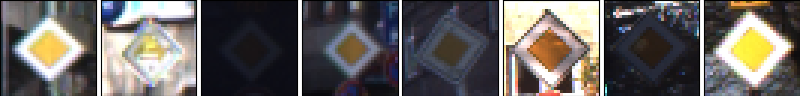
\includegraphics[width=1\textwidth]{images/desarrollo/imagenes/alemania/1__(13).png}
				%\end{center}
				%\begin{center}
				%\caption{\small{Priority road}}
				%\end{center}
				%\vspace{-1.5em}
			%\end{figure}
			
			\begin{figure}[H]
				\begin{center}
				
\includegraphics[width=1\textwidth]{images/desarrollo/imagenes/alemania/1__(23).png}
				\end{center}
				\begin{center}
				\caption{\small{Bumpy road}}
				\end{center}
				\vspace{-1.5em}
			\end{figure}

			\begin{figure}[H]
				\begin{center}
				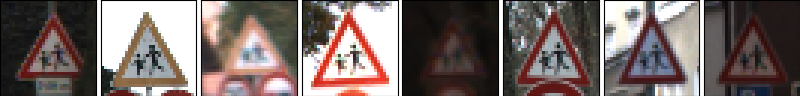
\includegraphics[width=1\textwidth]{images/desarrollo/imagenes/alemania/1__(29).png}
				\end{center}
				\begin{center}
				\caption{\small{Children crossing}}
				\end{center}
				\vspace{-1.5em}
			\end{figure}
			
			\begin{figure}[H]
				\begin{center}
				
\includegraphics[width=1\textwidth]{images/desarrollo/imagenes/alemania/1__(32).png}
				\end{center}
				\begin{center}
				\caption{\small{Wild animals crossing}}
				\end{center}
				\vspace{-1.5em}
			\end{figure}

			\begin{figure}[H]
				\begin{center}
				
\includegraphics[width=1\textwidth]{images/desarrollo/imagenes/alemania/1__(35).png}
				\end{center}
				\begin{center}
				\caption{\small{Turn left ahead}}
				\end{center}
				\vspace{-1.5em}
			\end{figure}


			\begin{figure}[H]
				\begin{center}
				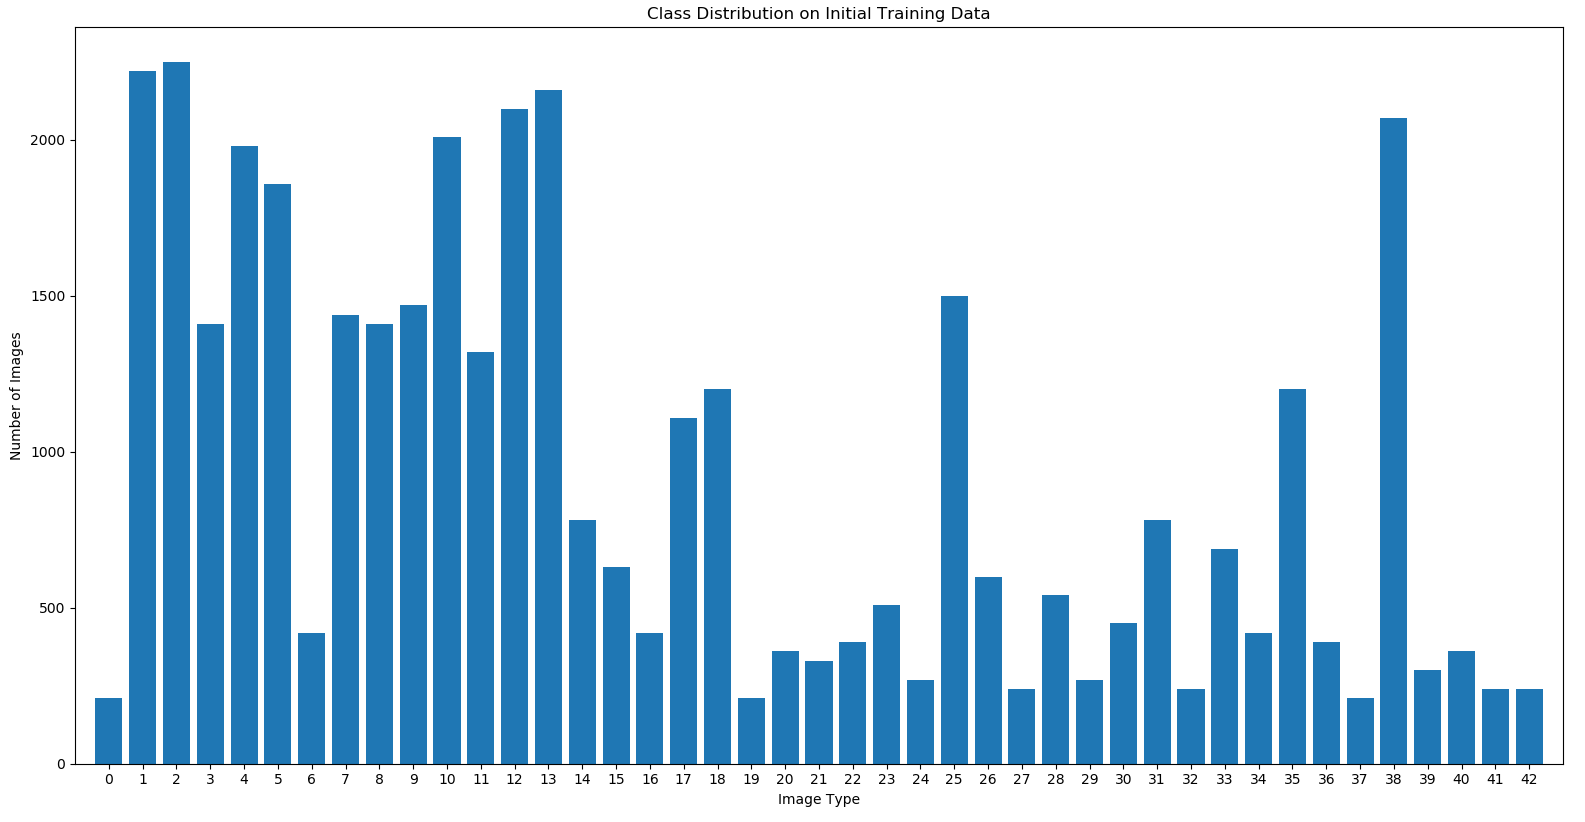
\includegraphics[width=1\textwidth]{images/desarrollo/histograms/initial39209}
				\end{center}
				\begin{center}
				\caption{\small{Distribución de ejemplos por señal para el entrenamiento(Total 39209)}}
				
			{\small{\fontsize{10}{16.8}\selectfont {Fuente propia}}}
				\end{center}
				\vspace{-1.5em}
			\end{figure}


		\subsubsection{Señales de Tránsito de Perú}

			En esta colección consta de un total de 614 imágenes distribuidas en 7 clases no necesariamente balanceadas con un tamaño de 60 x 60 pixeles.

			\begin{figure}[H]
				\begin{center}
				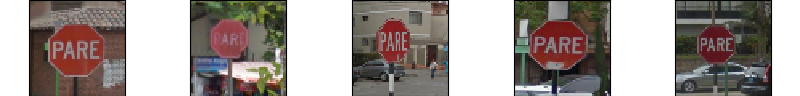
\includegraphics[width=1\textwidth]{images/desarrollo/imagenes/peru/1__(1).png}
				\end{center}
				\begin{center}
				\caption{\small{Pare}}
				\end{center}
				\vspace{-1.5em}
			\end{figure}

			\begin{figure}[H]
				\begin{center}
				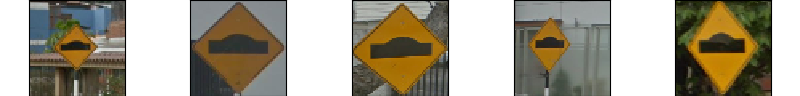
\includegraphics[width=1\textwidth]{images/desarrollo/imagenes/peru/1__(2).png}
				\end{center}
				\begin{center}
				\caption{\small{Resalto}}
				\end{center}
				\vspace{-1.5em}
			\end{figure}

			\begin{figure}[H]
				\begin{center}
				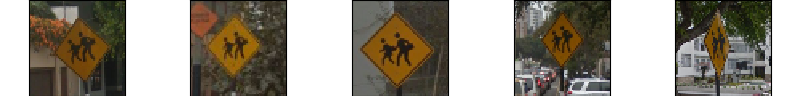
\includegraphics[width=1\textwidth]{images/desarrollo/imagenes/peru/1__(3).png}
				\end{center}
				\begin{center}
				\caption{\small{Zona Escolar}}
				\end{center}
				\vspace{-1.5em}
			\end{figure}

			\begin{figure}[H]
				\begin{center}
				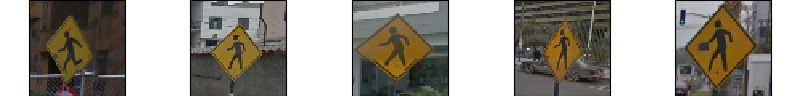
\includegraphics[width=1\textwidth]{images/desarrollo/imagenes/peru/1__(4).png}
				\end{center}
				\begin{center}
				\caption{\small{Peatones}}
				\end{center}
				\vspace{-1.5em}
			\end{figure}
			
			\begin{figure}[H]
				\begin{center}
				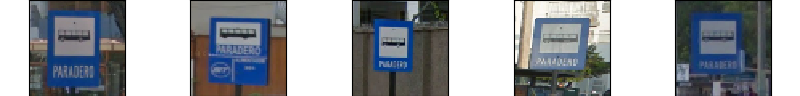
\includegraphics[width=1\textwidth]{images/desarrollo/imagenes/peru/1__(5).png}
				\end{center}
				\begin{center}
				\caption{\small{Paradero}}
				\end{center}
				\vspace{-1.5em}
			\end{figure}

			\begin{figure}[H]
				\begin{center}
				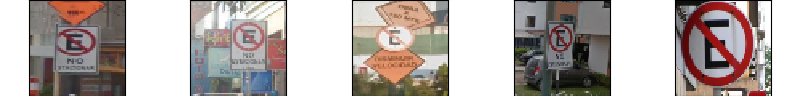
\includegraphics[width=1\textwidth]{images/desarrollo/imagenes/peru/1__(6).png}
				\end{center}
				\begin{center}
				\caption{\small{No Estacionar}}
				\end{center}
				\vspace{-1.5em}
			\end{figure}
			
			\begin{figure}[H]
				\begin{center}
				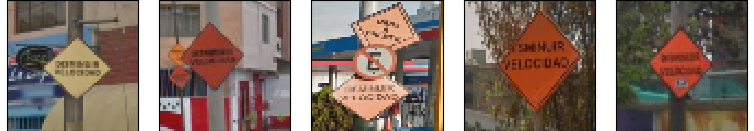
\includegraphics[width=1\textwidth]{images/desarrollo/imagenes/peru/1__(7).png}
				\end{center}
				\begin{center}
				\caption{\small{Disminuir Velocidad}}
				\end{center}
				\vspace{-1.5em}
			\end{figure}

			\begin{figure}[H]
				\begin{center}
				\includegraphics[width=1\textwidth]{images/desarrollo/histograms/inicioTrain614}
				\end{center}
				\begin{center}
				\caption{\small{Distribución de ejemplos por señal para el entrenamiento(Total 614)}}
				
			{\small{\fontsize{10}{16.8}\selectfont {Fuente propia}}}
				\end{center}
				\vspace{-1.5em}
			\end{figure}

			

	\subsection{Datos para el evaluación}
		Al igual que en el anterior punto, se obtienen un conjunto de menor cantidad de imágenes de señales de tránsito Alemán y Peruano, las cuales servirán para evaluar los modelos creados.

		\subsubsection{Señales de Tránsito de Alemania}
		Para la etapa de evaluación se cuenta con un conjunto de 12630 imágenes, de igual manera no necesariamente balanceadas y que no son utilizadas durante el proceso de entrenamiento para obtener resultados confiables a la hora de evaluar el resultado del entrenamiento. 

		\begin{figure}[H]
			%\begin{center}
			\includegraphics[width=1\textwidth]{images/desarrollo/histograms/initialTest12630}
			%\end{center}
			\begin{center}
			\caption{\small{Distribución de ejemplos por señal para la evaluación - Alemania}}
			
		{\small{\fontsize{10}{16.8}\selectfont {Fuente propia}}}
			\end{center}
			\vspace{-1.5em}
		\end{figure}

		\subsubsection{Señales de Tránsito de Perú}
		Para la etapa de evaluación se cuenta con un conjunto de 4698 imágenes, de igual manera no necesariamente balanceadas y que no son utilizadas durante el proceso de entrenamiento para obtener resultados confiables a la hora de evaluar el resultado del entrenamiento. 

		\begin{figure}[H]
			%\begin{center}
			\includegraphics[width=1\textwidth]{images/desarrollo/histograms/PeruinitialTest4698}
			%\end{center}
			\begin{center}
			\caption{\small{Distribución de ejemplos por señal para la evaluación - Perú}}
			
		{\small{\fontsize{10}{16.8}\selectfont {Fuente propia}}}
			\end{center}
			\vspace{-1.5em}
		\end{figure}

	\subsection{Proceso de Aumento de Datos(Data Augmentation)}

		Las redes convolucionales durante el aprendizaje profundo requieren una gran cantidad de datos para conseguir realizar un mejor entrenamiento(aprendizaje) y obtener un modelo que generalice eficazmente. Muchas veces esta recopilación de datos suele ser costosa y laboriosa es por eso que el proceso de Data Augmentation ayuda a superar este problema a través del uso de métodos o técnicas de procesamiento de imágenes. Recientemente se ha utilizado ampliamente el aumento de datos genéricos para mejorar el rendimiento de las Redes Neuronales Convolucionales,\citep{DL_augmentData}. 

		\begin{figure}[H]
		\begin{center}
		\includegraphics[width=0.5\textwidth ]{images/desarrollo/Augment/exampleaug}
		\end{center}
		\begin{center}
		\caption{\small{El aumento de datos infla artificialmente los conjuntos de datos usando transformaciones que preservan las categorias de los objetos}}
		{\small{\citep{DL_augmentData}}}
		\end{center}
		\vspace{-1.5em}
		\end{figure}


		Son utilizadas las siguientes técnicas:
		
		
		\subsubsection{Flipping}
		
			Primero, vamos a aplicar un par de trucos para extender nuestros datos volteando. Algunas señales de tráfico son invariantes para voltear horizontal y / o verticalmente, lo que básicamente significa que podemos voltear una imagen y todavía debe clasificarse como perteneciente a la misma clase.

			Esta técnica solo fue utilizada para el dataset de señales de Tránsito de Alemania.
			
			\begin{multicols}{2}
				
				\underline{Flipping horizontal:}
				\begin{figure}[H]
					\begin{center}
					\includegraphics[height=14.5cm ]{images/desarrollo/Augment/flippedHorizontally}
					\end{center}
					\begin{center}
					\caption{\small{Imágenes volteadas horizontalmente}}
					
				{\small{\fontsize{10}{16.8}\selectfont {Fuente propia}}}
					\end{center}
					\vspace{-1.5em}
				\end{figure}

			%second column
			
				\underline{Flipping Vertical:}
				\begin{figure}[H]
					\begin{center}
					\includegraphics[height=13cm]{images/desarrollo/Augment/flippableVertically}
					\end{center}
					\begin{center}
					\caption{\small{Imágenes volteadas verticalmente}}
					
				{\small{\fontsize{10}{16.8}\selectfont {Fuente propia}}}
					\end{center}
					\vspace{-1.5em}
				\end{figure}

			\end{multicols}

			\newpage
			\underline{Flipping Horizontal y Vertical:}
			\begin{figure}[H]
				%\begin{center}
				\includegraphics[width=0.9\textwidth]{images/desarrollo/Augment/flippable_both}
				%\end{center}
				\begin{center}
				\caption{\small{Imágenes volteadas primero horizontal y luego verticalmente}}
				
				{\small{\fontsize{10}{16.8}\selectfont {Fuente propia}}}
				\end{center}
				\vspace{-1.5em}
			\end{figure}

			Incluso, hay signos que luego de voltearse, deben clasificarse como un signo de alguna otra clase. Esto sigue siendo útil, ya que podemos utilizar los datos de estas clases para ampliar sus contrapartes.
			\begin{figure}[H]
				\begin{center}
				\includegraphics[height=10.5cm ]{images/desarrollo/Augment/cross_flippable}
				\end{center}
				\begin{center}
				\caption{\small{Imágenes que volteadas horizontal o verticalmente, cambian su categoría}}
				
				{\small{\fontsize{10}{16.8}\selectfont {Fuente propia}}}
				\end{center}
				\vspace{1.5em}
			\end{figure}


			Finalmente obtenemos una nueva distribución de datos luego de haber aplicado flipping a ciertas imagenes. Esta distribución consta de 63538 imágenes.
			\begin{figure}[H]
				\begin{center}
				\includegraphics[width=1\textwidth]{images/desarrollo/histograms/train_flipped63538}
				\end{center}
				\begin{center}
				\vspace{1em}
				\caption{\small{Distribución de categoría, luego de aplicar el Flip(en sus distintos tipos)- Señales de Alemania}}
				
				{\small{\fontsize{10}{16.8}\selectfont {Fuente propia}}}
				\end{center}
				\vspace{-1.5em}
			\end{figure}

		Las siguientes técnicas fueron utilizadas para el dataset de señales de Tránsito de Alemania y de Perú.
		
		\subsubsection{Projection(Proyección)}
			Implica mover la imagen a lo largo de la dirección X o Y (o ambas). Este método de aumento es muy útil ya que la mayoría de los objetos se pueden ubicar en casi cualquier lugar de la imagen. Esto obliga a la red neuronal convolucional a buscar en todas partes.
			Los márgenes de proyección se asignan al azar en un rango que depende del tamaño de la imagen. La transformación de proyección parece también ocuparse de escalar al azar a medida que colocamos al azar las esquinas de la imagen en un rango [-delta, +delta].



			\begin{figure}[H]
				\begin{center}
				\includegraphics[width=1\textwidth,height=10cm]{images/desarrollo/Augment/projection_transform2}
				\includegraphics[width=1\textwidth,height=10cm]{images/desarrollo/Augment/projection_transform}
				\end{center}
				\begin{center}
				\vspace{1em}
				\caption{\small{Ejemplo de cinco proyecciones por cada imagen - Dataset Alemania}}
				
			{\small{\fontsize{10}{16.8}\selectfont {Fuente propia}}}
				\end{center}
				\vspace{-1.5em}
			\end{figure}
		\newpage
		\subsubsection{Rotation(Rotación)}
			\vspace{-1.5em}
			Aplica la rotación aleatoria en un rango de grados definido(hasta 30º) a un subconjunto aleatorio de imágenes.
	        El rango en sí está sujeto a escala dependiendo de la intensidad de aumento.

	        \begin{figure}[H]
				\begin{center}
				\includegraphics[width=1\textwidth,height=9cm]{images/desarrollo/Augment/fixedrotation}
				\end{center}
				\begin{center}
				\caption{\small{Ejemplo de cinco rotaciones por cada imagen - Dataset Alemania}}
				
			{\small{\fontsize{10}{16.8}\selectfont {Fuente propia}}}
				\end{center}
				\vspace{-1.5em}
			\end{figure}
			%\vspace{-2.5em}
	    

	    \subsubsection{Zoom}
	    	\vspace{-1.5em}
	    	Acerca(zoom in) o aleja(zoom out) la imagen  tratando de preservar el fondo.

	    	%\begin{figure}[H]
			%	\begin{center}
			%	\includegraphics[width=1\textwidth,height=10cm]{images/desarrollo/Augment/zoom_normal}
			%	\end{center}
			%\end{figure}

			\begin{figure}[H]
				\begin{center}
				\includegraphics[width=1\textwidth,height=8cm]{images/desarrollo/Augment/zoom_inv}
				\end{center}
				\begin{center}
				\vspace{0.5em}
				\caption{\small{Ejemplo de cinco aplicaciones de zoom(in/out) por cada imagen - Dataset Alemania}}
				
			{\small{\fontsize{10}{16.8}\selectfont {Fuente propia}}}
				\end{center}
				\vspace{-1.5em}
			\end{figure}


		\subsubsection{Equalizacion del histograma}
			Aumenta el contraste global de muchas imágenes, especialmente cuando los datos utilizables de la imagen están representados por valores de contraste cercanos. Esto permite que áreas de menor contraste local puedan obtener un mayor contraste. La ecualización del histograma logra esto al distribuir eficazmente los valores de intensidad más frecuentes.

			\begin{figure}[H]
				\begin{center}
				\includegraphics[height=9.5cm]{images/desarrollo/Augment/equalize_hist2_wo_Norm_woRepetition}
				\end{center}
				\begin{center}
				\caption{\small{Ilustración de un modelo de aprendizaje profundo}}
				
			{\small{\fontsize{10}{16.8}\selectfont {Fuente propia}}}
				\end{center}
				\vspace{-1.5em}
			\end{figure}
		
		
		%	\begin{figure}[H]
				%\begin{center}
		%		\includegraphics[width=0.9\textwidth,height=11cm]{images/desarrollo/Augment/AllTogether_ramdoly_mixed2}
				%\end{center}
		%		\begin{center}
		%		\caption{\small{Ilustración de un modelo de aprendizaje profundo}}
		%		
		%	{\small{\fontsize{10}{16.8}\selectfont {Fuente propia}}}
		%		\end{center}
		%		\vspace{-1.5em}
		%	\end{figure}

	\newpage
	\subsection{Dataset final para el Entrenamiento}
		Finalmente, luego de haber aplicado de manera secuencial y/o aleatoriamente estas tecnicas a cada una de las imágenes, obtenemos nuevas distribuciones de datos. 
		\subsubsection{Señales de Tránsito de Alemania - Dataset Balanceado }
			En una se tiene un conjunto balanceado de datos con {\bf 270900 imágenes}.
			\begin{figure}[H]
				%\begin{center}
				\includegraphics[width=1\textwidth, height=8.5cm]{images/desarrollo/histograms/train_extended_balanced270900}
				%\end{center}
				\begin{center}
				\caption{\small{Dataset balanceado(cada categoría posee igual cantidad de imágenes)}}
				
				{\small{\fontsize{10}{16.8}\selectfont {Fuente propia}}}
				\end{center}

			\end{figure}

			Teniendo en cuenta lo descrito en la \textbf{Seccion 2.3.4 (Validación Cruzada)}, para la etapa del entrenamiento, el conjunto de datos Balanceados compuesto por 270900 imágenes fue dividido en un subconjunto de entrenamiento y otro para validación, con la siguiente distribución:
			\vspace{1.5em}
			\begin{table}[H]
				\caption{\small{Distribución Entrenamiento y Validación Dataset Balanceado - Señales de Tránsito de Alemania}}
				\begin{center}
				\begin{tabular}{|>{\scriptsize}c|>{\scriptsize}c|}
				\hline
				{\ul \textbf{CONJUNTO DE DATOS}}           & {\ul \textbf{CANTIDAD IMÁGENES}}                \\ \hline
				\textbf{Entrenamiento}                    & \text{203175 (75\%)}                       \\ \hline
				\textbf{Validación}                       & \text{67725 (25\%)}                    \\ \hline
				\end{tabular}
				\end{center}
			\end{table}

	%---------------------------------------------------------------------------------------------------------------------------------------------------------
	
		\subsubsection{Señales de Tránsito de Perú - Dataset No Balanceado}
			Con el objetivo de obtener una gran cantidad de datos, para el Dataset de señales de Tránsito del Perú, por cada imágen fueron creadas 50 nuevas imágenes, obteniéndose {\bf 31314 imágenes}.
			\begin{figure}[H]
				%\begin{center}
				\includegraphics[width=1\textwidth, height=8.5cm]{images/desarrollo/histograms/train_extended_per_51_31314}
				%\end{center}
				\begin{center}
				\caption{\small{Dataset no balanceado - Señales de Tránsito de Perú}}
				
				{\small{\fontsize{10}{16.8}\selectfont {Fuente propia}}}
				\end{center}
			\end{figure}

			Para este caso, el dataset aumentado se configuró con una distribución de datos para entrenamiento, validación y evaluación: 
			\vspace{1.5em}
			\begin{table}[H]
				\caption{\small{Distribución Entrenamiento y Validación Dataset no Balanceado - Señales de Tránsito de Perú}}
				\begin{center}
				\begin{tabular}{|>{\scriptsize}c|>{\scriptsize}c|}
				\hline
				{\ul \textbf{CONJUNTO DE DATOS}}           & {\ul \textbf{CANTIDAD IMÁGENES}}     \\ \hline
				\textbf{Entrenamiento}                    & \text{23485 (75\%)}                   \\ \hline
				\textbf{Validación}                       & \text{3131 (10\%)}                    \\ \hline
				\textbf{Evaluación}                       & \text{4698 (15\%)}                    \\ \hline
				\end{tabular}
				\end{center}
			\end{table}

	%---------------------------------------------------------------------------------------------------------------------------------------------------------
	\newpage
	\subsection{Pre-procesamiento de Imágenes(Normalization)}
		Existe una técnica de procesamiento de imágenes por computadora que se utiliza para mejorar el contraste en las imágenes denominada Ecualización Adaptativa del Histograma(AHE por sus siglas en inglés). Difiere de la ecualización de histograma ordinaria en el sentido de que el método adaptativo computa varios histogramas, cada uno correspondiente a una sección distinta de la imagen, y los utiliza para redistribuir los valores de luminosidad de la imagen. Por lo tanto, es adecuado para mejorar el contraste local y mejorar las definiciones de los bordes en cada región de una imagen. Sin embargo, AHE tiene una tendencia a amplificar el ruido en regiones relativamente homogéneas de una imagen. Una variante de la ecualización de histograma adaptativo llamada ecualización de histograma adaptativo limitado por contraste (CLAHE por sus siglas en inglés) evita que se genere esto al limitar la amplificación.

		En esta investigación, aplicaremos la técnica CLAHE, un algoritmo para la mejora del contraste local, que utiliza histogramas calculados sobre diferentes regiones en una imagen. Utilizado frecuentemente para mejorar el nivel de visibilidad de una imagen o video con niebla ya que permite mejorar los detalles locales incluso en regiones que son más oscuras o más claras que la mayoría de regiones de la imagen. Este algoritmo mejorará aún más la extracción de características de cada imágen.\citep{CLAHE}

			\begin{figure}[H]
			%\begin{center}
			\includegraphics[width=1\textwidth]{images/desarrollo/Normalization_Processing/norm_test1}
			\includegraphics[width=1\textwidth]{images/desarrollo/Normalization_Processing/norm_test2}
			%\end{center}
			\begin{center}
			\caption{\small{Imágenes a las cuales se le aplicaron la técnica CLAHE }}
			
			{\small{\fontsize{10}{16.8}\selectfont {Fuente propia}}}
			\end{center}
			\vspace{-1.5em}
			\end{figure}
		
		Por otra parte, para convertir un color de un espacio de color basado en un modelo de color RGB típico de gamma comprimido (no lineal) a una representación en escala de grises de su luminancia, primero se debe eliminar la función de compresión gamma mediante la expansión gamma (linealización) para transformar la imagen en un RGB lineal espacio de color, de modo que la suma ponderada apropiada se puede aplicar a los componentes de color lineales ($R_{linear} , G_{linear} , B_{linear}$) para calcular la luminancia lineal $Y_{linear}$.

		Para imágenes en espacios de color como Y'UV y sus derivados, que se usan en sistemas de TV y video a color estándar como PAL, SECAM y NTSC, un componente de luma no lineal ($Y'$) se calcula directamente a partir de intensidades primarias comprimidas con gamma como una suma ponderada, que aunque no es una representación perfecta de la luminancia colorimétrica, puede calcularse más rápidamente sin la expansión gamma y sin la compresión utilizadas en los cálculos fotométricos o colorimétricos,\citep{POYNTON2003257}. En los modelos utilizados por PAL y NTSC para conseguir tener las imágenes en escala de grises, el componente rec601 luma ($Y'$) se calcula como: \begingroup\makeatletter\def\f@size{14.8}\check@mathfonts	$Y' = 0.299R' + 0.587G' +0.114B'$ \endgroup

		Pierre Sermanet y Yann LeCun mencionaron en su artículo \citep{LeCun}, que el uso de canales de color no pareció mejorar mucho las cosas. Además, debido a diversas condiciones o problemas de iluminación, no es adecuado procesar directamente las imágenes que se capturan a través de la cámara o sensores de imágenes, es por ello que en esta investigación {\bf se usará un solo canal} en el modelo, es decir las imágenes estarán en escala de grises en lugar de tener 3 canales de colores.
		
			\begin{figure}[H]
			\begin{center}
			\includegraphics[width=0.7\textwidth]{images/desarrollo/Normalization_Processing/proc_test1}
			\includegraphics[width=0.7\textwidth]{images/desarrollo/Normalization_Processing/proc_test2}
			\end{center}
			\begin{center}
			\caption{\small{Imágenes procesadas en escala de grises}}
			
			{\small{\fontsize{10}{16.8}\selectfont {Fuente propia}}}
			\end{center}
			\vspace{-1.5em}
			\end{figure}
			\newpage
	

\section{Arquitectura del Modelo}


	Los hiperparámetros engloban funciones, variables y constantes utilizadas durante la construcción de las diferentes arquitecturas; estas varían, sin embargo siguiendo conceptos teóricos, antecedentes(investigaciones previas) y sobretodo despues de algunas pruebas realizadas, los siguientes hiperparámetros fueron seleccionados de manera específica:
		% Please add the following required packages to your document preamble:
		% \usepackage{multirow}
		%\usepackage[table,xcdraw]{xcolor}
		% If you use beamer only pass "xcolor=table" option, i.e. \documentclass[xcolor=table]{beamer}
		% \usepackage[normalem]{ulem}
		% \useunder{\uline}{\ul}{}
		\begin{table}[H]
			\begin{center}
			\caption{\small{Hiperparámetros del Modelo}}
			\begin{tabular}{|>{\scriptsize}c|>{\scriptsize}c|>{\scriptsize}c|>{\scriptsize}c|}
			\hline
			{\ul \textbf{HIPERPARÁMETROS}}  & {\ul \textbf{TIPO}}       & {\ul \textbf{HIPERPARÁMETROS}}        & {\ul \textbf{TIPO}}        \\ \hline
			{\textbf{Inicialización de Pesos}}                     		& {\textit{Xavier}}  				  &
			\textbf{Tasa de Aprendizaje}                                & \textit{0.0005}                    \\ \hline
			\textbf{Alg. de Optimización}                               & \textit{Optimizador Adam}          &
			\textbf{Método de Validación}                               & \textit{Entropía Cruzada}          \\ \hline
			\textbf{Fun. Activ. Capas Convolucionales}        			& \textit{RELU y DropOut}                      &
			\textbf{Fun. Activ. Capas Totalmente Conectadas} 			& \textit{Func. Softmax}           \\ \hline
			\textbf{Método de Regularización}                           &\textit{L2 Lasso(lambda = 0.0001)} &
			\textbf{Épocas}                                             &\textit{100}		 				\\ \hline
			\end{tabular}
			\end{center}
		\end{table}
		\vspace{-1.5em}

		Recordemos que en cada época se procesa el dataset completo de imágenes, por lo que cada época es igual : \begingroup\makeatletter\def\f@size{11}\check@mathfonts	$Epoca = Mini batch \times iteraciones$ \endgroup

		Sin embargo debido a que se tiene dos distintos datasets para el entrenamiento \textbf{(Seccion 4.1.4 - Dataset final para el Entrenamiento)}, el tamaño del Minibatch cambiará respecto al tamaño del dataset y por ende también será diferente la cantidad de iteraciones ejecutadas durante 100 épocas de entrenamiento.                        
		
		%\begin{center}\end{center}

		\begin{table}[H]
			\begin{center}
			\caption{\small{Minibatch e iteraciones en el Dataset de Señales de Tránsito de Alemania Balanceado}}
			\begin{tabular}{|>{\scriptsize}c|>{\scriptsize}c|>{\scriptsize}c|>{\scriptsize}c|}
			\hline
			\textbf{Imágenes totales }                 &\textit{203175}                       \\ \hline
			\textbf{Iteraciones por Época}                 &\textit{387}                             \\ \hline
			\textbf{Tamaño del Mini-batch}                 &\textit{525 imágenes analizadas por iteración}                       \\ \hline
			\textbf{Épocas entrenadas}                &\textit{100 épocas (38700 iter.)}                       \\ \hline
			\end{tabular}
			\end{center}
		\end{table}


		\begin{table}[H]
			\begin{center}
			\caption{\small{Minibatch e iteraciones en el Dataset de Señales de Tránsito de Peru No Balanceado}}
			\begin{tabular}{|>{\scriptsize}c|>{\scriptsize}c|>{\scriptsize}c|>{\scriptsize}c|}
			\hline
			\textbf{Imágenes totales }                 &\textit{23485}                       \\ \hline
			\textbf{Iteraciones por Época}                 &\textit{77}                             \\ \hline
			\textbf{Tamaño del Mini-batch}                 &\textit{305 imágenes analizadas por iteración}                       \\ \hline
			\textbf{Épocas entrenadas}                &\textit{100 épocas (7700 iter.)}                       \\ \hline
			\end{tabular}
			\end{center}
		\end{table}

	En esta investigación se implementó el modelo de redes neuronales convolucionales(CNN) donde las capas convolucionales iniciales de la red extraen características de la imagen(feature extractor), mientras que las capas totalmente conectadas predicen las probabilidades de salida(classifier).

		\begin{figure}[H]
		%\begin{center}
		\includegraphics[width=1\textwidth]{images/desarrollo/networkArquitec/tempGeneralCNNmodel}
		%\end{center}
		\begin{center}
		\caption{\small{Arquitectura de la CNN}}
		
		{\small{\fontsize{10}{16.8}\selectfont {Extreme Learning Classifier}}}
		\end{center}
		\vspace{-1.5em}
		\end{figure}

	La arquitectura de la red está inspirada en el arquitectura Inception \citep{Inception} y en la arquitectura AlexNet\citep{Krizhevsky2012} para la clasificación de imágenes. En la arquitectura Inception, el modelo creado es denominado GoogLeNet, similar a AlexNet donde varios módulos iniciales son apilados uno sobre el otro para producir el resultado final. En el módulo de inicio, en ese tipo de red, se usaron diversos tamaños de filtros convolucionales para capturar características de diferente abstracción. El alto nivel de abstracción se captura con filtros de mayor tamaño y el de un nivel inferior con filtros de menor tamaño. Procesando información visual a diferentes escalas y al concatenarlas se obtiene un nivel eficiente de abstracción. 
	%%%	Dado que aplicar directamente más filtros convolucionales con datos de imagen y concatenarlos es computacionalmente costoso, en el modelo Inception finalmente se usaron filtros de reducción de dimensionalidad(pooling/acumulación). Además de ser muy exitoso para la reducción de dimensionalidad, estos filtros también llegan a ser útiles como activación lineal rectificada. La arquitectura de inicio es eficiente en términos de complejidad computacional con respecto al número de unidades en cada etapa. \citep{Mrinal2016}.las características abstractas locales desempeñan un papel importante. Las señales que pertenecen al mismo grupo tienen una ligera diferencia en la estructura local entre sí, lo que dificulta su distinción. Por lo que se optó por agregar un kernel de reducción convolucional de 3 × 3 extra con acumulación máxima en la parte superior para capturar la estructura local discriminativa al comienzo mismo. Los signos pertenecientes a diferentes grupos tienen una abstracción global que se puede capturar utilizando un núcleo de reducción convolucional de 5 × 5.

	Para la clasificación de señales de tránsito en esta investigación se utilizó una versión modificada de las arquitecturas antes mencionadas. Se incorporó {\bf funciones de escala-múltiple} \citep{Multi_scale_feat}, lo que significa que la salida de las capas convolucionales no solo se envía a la capa posterior, sino que también se ramifica y se introduce al clasificador (capa totalmente conectada). La razón detrás de esto es que cuando el clasificador está tomando una decisión basada en convoluciones, podría encontrar que la salida de la primera o segunda capa convolucional también es útil. Básicamente con las características de escala múltiple depende del clasificador qué nivel de abstracción usar, ya que tiene acceso a las salidas de todas las capas convolucionales, es decir,características en todos los niveles de abstracción. Estas capas ramificadas se someten a un pooling máximo adicional, de modo que todas las convoluciones se submuestrean proporcionalmente antes de entrar en el clasificador. Así se garantiza que todas las funciones de escala múltiple experimenten la misma cantidad de máximo aprovechamiento.
	
	\subsection{Diseño de la Red}
	
	Teniendo en cuenta lo descrito en la {\bf seccion 2.2 (Figura 2.5)}, para describir las capas convolucionales se utilizará la terminología compleja(cada capa tiene múltiples etapas).
	
		\begin{figure}[H]
		%\begin{center}
		\includegraphics[width=1\textwidth]{images/desarrollo/networkArquitec/designNet}
		%\end{center}
		\begin{center}
		\caption{\small{Modelo del diseño de la Red propuesta}}
		
		{\small{\fontsize{10}{16.8}\selectfont {Fuente propia}}}
		\end{center}
		\vspace{-1.5em}
		\end{figure}


	Para el proceso de entrenamiento fueron tomados en cuenta 5 diferentes diseños. Estos fueron ejectudados durante el entrenamiento del dataset que contiene señales de tránsito de Alemania y Perú.

	Estos 5 modelos son descritos a continuación.
		\vspace{-1.5em}
		\subsubsection{Diseño A} 
			Diseño compuesto de 2 capas convolucionales y 2 capas totalmente conectadas.
			% Please add the following required packages to your document preamble:
			% \usepackage{multirow}
			% \usepackage[table,xcdraw]{xcolor}
			% If you use beamer only pass "xcolor=table" option, i.e. \documentclass[xcolor=table]{beamer}
			\begin{itemize}
			\item \underline{Dataset de Alemania}			
				\begin{table}[H]
				\begin{center}
				\caption{\small{Diseño A - Dataset de Imágenes de Alemania}}
				\begin{tabular}{|>{\scriptsize}c|>{\scriptsize}c>{\scriptsize}c>{\scriptsize}c>{\scriptsize}c>{\scriptsize}c|>{\scriptsize}c|}
				\hline
				{\color[HTML]{000000} \textbf{Capa}} & {\color[HTML]{000000} \textbf{Entrada}} & {\color[HTML]{000000} \textbf{Tipo}} & {\color[HTML]{000000} \textbf{\begin{tabular}[c]{@{}c@{}}Número de\\ (kernels/filtros)\end{tabular}}} & {\color[HTML]{000000} \textbf{Padding}} & {\textbf{Salida}} & {\textbf{Func.Esc.Múltiple}}\\ \hline

				 & 1 de 32 x 32 neuronas & Conv(DropOut : 0.8) & 32 de 3 x 3 & Activo & 32 de 32 x 32 neuronas & --\\ 
				\multirow{-2}{*}{1} &  32 de 32 x 32 neuronas &  Max Pool &  32 de 2 x 2 &  Inactivo & 32 de 16 x 16 neuronas & {\cellcolor[HTML]{DAE8FC}(Kernel = 2) 32 de 8x8}\\ \hline
				 & 32 de 16 x 16 neuronas & Conv(DropOut : 0.7) & 64 de 5 x 5 & Activo & 32 de 16 x 16 neuronas & --\\ 
				\multirow{-2}{*}{2} &  64 de 16 x 16 neuronas &  Max Pool &  64 de 2 x 2 &  Inactivo & 64 de 8 x 8 neuronas & {\cellcolor[HTML]{DAE8FC}(Kernel = 1) 64 de 8x8}\\ \hline
				3 &  {\cellcolor[HTML]{DAE8FC}6144 neuronas} &  F.C.(DropOut : 0.5) &  3072 neuronas &  -- & 43 neuronas & --\\ \hline

				\end{tabular}
				\end{center}
				\end{table}
			\vspace{-1.5em}
			\item \underline{Dataset del Perú}
				\begin{table}[H]
				\begin{center}
				\caption{\small{Diseño A - Dataset de Imágenes de Perú}}
				\begin{tabular}{|>{\scriptsize}c|>{\scriptsize}c>{\scriptsize}c>{\scriptsize}c>{\scriptsize}c>{\scriptsize}c|>{\scriptsize}c|}
				\hline
				{\color[HTML]{000000} \textbf{Capa}} & {\color[HTML]{000000} \textbf{Entrada}} & {\color[HTML]{000000} \textbf{Tipo}} & {\color[HTML]{000000} \textbf{\begin{tabular}[c]{@{}c@{}}Número de\\ (kernels/filtros)\end{tabular}}} & {\color[HTML]{000000} \textbf{Padding}} & {\textbf{Salida}} & {\textbf{Func.Esc.Múltiple}}\\ \hline

				 & 1 de 60 x 60 neuronas & Conv(DropOut : 0.8) & 32 de 3 x 3 & Activo & 32 de 60 x 60 neuronas & --\\ 
				\multirow{-2}{*}{1} &  32 de 60 x 60 neuronas &  Max Pool &  32 de 2 x 2 &  Inactivo & 32 de 30 x 30 neuronas & {\cellcolor[HTML]{DAE8FC}(Kernel = 2) 32 de 15x15}\\ \hline
				 & 32 de 30 x 30 neuronas & Conv(DropOut : 0.7) & 64 de 5 x 5 & Activo & 64 de 30 x 30 neuronas & --\\ 
				\multirow{-2}{*}{2} &  64 de 30 x 30 neuronas &  Max Pool &  64 de 2 x 2 &  Inactivo & 64 de 15 x 15 neuronas & {\cellcolor[HTML]{DAE8FC}(Kernel = 1) 64 de 15x15}\\ \hline
				3 &  {\cellcolor[HTML]{DAE8FC}21600 neuronas} &  F.C.(DropOut : 0.5) &  3072 neuronas &  -- & 7 neuronas & --\\ \hline

				\end{tabular}
				\end{center}
				\end{table}

			\end{itemize}
		%------------------------------------------------------------------------------------------------------------------------------------------------------------
		\subsubsection{Diseño B}
		Diseño compuesto de 3 capas convolucionales y 2 capas totalmente conectadas.
			\begin{itemize}
			\item \underline{Dataset de Alemania}		
				\begin{table}[H]
				\begin{center}
				\caption{\small{Diseño B - Dataset de Imágenes de Alemania}}
				\begin{tabular}{|>{\scriptsize}c|>{\scriptsize}c>{\scriptsize}c>{\scriptsize}c>{\scriptsize}c>{\scriptsize}c|>{\scriptsize}c|}
				\hline
				{\color[HTML]{000000} \textbf{Capa}} & {\color[HTML]{000000} \textbf{Entrada}} & {\color[HTML]{000000} \textbf{Tipo}} & {\color[HTML]{000000} \textbf{\begin{tabular}[c]{@{}c@{}}Número de\\ (kernels/filtros)\end{tabular}}} & {\color[HTML]{000000} \textbf{Padding}} & {\textbf{Salida}} & {\textbf{Func.Esc.Múltiple}}\\ \hline

				 & 1 de 32 x 32 neuronas & Conv(DropOut : 0.8) & 32 de 3 x 3 & Activo & 32 de 32 x 32 neuronas & --\\ 
				\multirow{-2}{*}{1} &  32 de 32 x 32 neuronas &  Max Pool &  32 de 2 x 2 &  Inactivo & 32 de 16 x 16 neuronas & {\cellcolor[HTML]{DAE8FC}(Kernel = 4) 32 de 4x4}\\ \hline
				 & 32 de 16 x 16 neuronas & Conv(DropOut : 0.7) & 64 de 5 x 5 & Activo & 64 de 16 x 16 neuronas & --\\ 
				\multirow{-2}{*}{2} &  64 de 16 x 16 neuronas &  Max Pool &  64 de 2 x 2 &  Inactivo & 64 de 8 x 8 neuronas & {\cellcolor[HTML]{DAE8FC}(Kernel = 2) 64 de 4x4}\\ \hline			
				{\cellcolor[HTML]{ffb3b3}} & 64 de 8 x 8 neuronas & Conv(DropOut : 0.6) & 128 de 5 x 5 & Activo & 128 de 8 x 8 neuronas & --\\ 			
				{\cellcolor[HTML]{ffb3b3} \multirow{-2}{*}{3}} &  128 de 8 x 8 neuronas &  Max Pool &  128 de 2 x 2 &  Inactivo & 128 de 4 x 4 neuronas & {\cellcolor[HTML]{DAE8FC} (Kernel = 1) 128 de 4x4 }\\ \hline
				4 &  {\cellcolor[HTML]{DAE8FC}3584 neuronas} &  F.C.(DropOut : 0.5) &  1024 neuronas &  -- & 43 neuronas & --\\ \hline
				\end{tabular}
				\end{center}
				\end{table}
			\vspace{2em}
			\item \underline{Dataset del Perú}
				\begin{table}[H]
				\begin{center}
				\caption{\small{Diseño B - Dataset de Imágenes de Alemania}}
				\begin{tabular}{|>{\scriptsize}c|>{\scriptsize}c>{\scriptsize}c>{\scriptsize}c>{\scriptsize}c>{\scriptsize}c|>{\scriptsize}c|}
				\hline
				{\color[HTML]{000000} \textbf{Capa}} & {\color[HTML]{000000} \textbf{Entrada}} & {\color[HTML]{000000} \textbf{Tipo}} & {\color[HTML]{000000} \textbf{\begin{tabular}[c]{@{}c@{}}Número de\\ (kernels/filtros)\end{tabular}}} & {\color[HTML]{000000} \textbf{Padding}} & {\textbf{Salida}} & {\textbf{Func.Esc.Múltiple}}\\ \hline

				 & 1 de 60 x 60 neuronas & Conv(DropOut : 0.8) & 32 de 3 x 3 & Activo & 32 de 60 x 60 neuronas & --\\ 
				\multirow{-2}{*}{1} &  32 de 60 x 60 neuronas &  Max Pool &  32 de 2 x 2 &  Inactivo & 32 de 30 x 30 neuronas & {\cellcolor[HTML]{DAE8FC}(Kernel = 4) 32 de 7x7}\\ \hline
				 & 32 de 30 x 30 neuronas & Conv(DropOut : 0.7) & 64 de 5 x 5 & Activo & 64 de 30 x 30 neuronas & --\\ 
				\multirow{-2}{*}{2} &  64 de 30 x 30 neuronas &  Max Pool &  64 de 2 x 2 &  Inactivo & 64 de 15 x 15 neuronas & {\cellcolor[HTML]{DAE8FC}(Kernel = 2) 64 de 7x7}\\ \hline			
				{\cellcolor[HTML]{ffb3b3}} & 64 de 15 x 15 neuronas & Conv(DropOut : 0.6) & 128 de 5 x 5 & Activo & 128 de 15 x 15 neuronas & --\\ 			
				{\cellcolor[HTML]{ffb3b3} \multirow{-2}{*}{3}} &  128 de 15 x 15 neuronas &  Max Pool &  128 de 2 x 2 &  Inactivo & 128 de 7 x 7 neuronas & {\cellcolor[HTML]{DAE8FC} (Kernel = 1) 128 de 7x7 }\\ \hline
				4 &  {\cellcolor[HTML]{DAE8FC}10976 neuronas} &  F.C.(DropOut : 0.5) &  1024 neuronas &  -- & 7 neuronas & --\\ \hline
				\end{tabular}
				\end{center}
				\end{table}

				\end{itemize}
		%------------------------------------------------------------------------------------------------------------------------------------------------------------
		\vspace{-2.2em}
		\subsubsection{Diseño C} %model4
			\vspace{-1.2em}
			Diseño compuesto de 3 capas convolucionales y 2 capas totalmente conectadas. Variando el número de kernels en la 2da capa convolucional.
			
			\begin{itemize}
			\item \underline{Dataset de Alemania}		
				\begin{table}[H]
				\begin{center}
				\caption{\small{Diseño C - Dataset de Imágenes de Alemania}}
				\begin{tabular}{|>{\scriptsize}c|>{\scriptsize}c>{\scriptsize}c>{\scriptsize}c>{\scriptsize}c>{\scriptsize}c|>{\scriptsize}c|}
				\hline
				{\color[HTML]{000000} \textbf{Capa}} & {\color[HTML]{000000} \textbf{Entrada}} & {\color[HTML]{000000} \textbf{Tipo}} & {\color[HTML]{000000} \textbf{\begin{tabular}[c]{@{}c@{}}Número de\\ (kernels/filtros)\end{tabular}}} & {\color[HTML]{000000} \textbf{Padding}} & {\textbf{Salida}} & {\textbf{Func.Esc.Múltiple}}\\ \hline

				 & 1 de 32 x 32 neuronas & Conv(DropOut : 0.8) & 32 de 3 x 3 & Activo & 32 de 32 x 32 neuronas & --\\ 
				\multirow{-2}{*}{1} &  32 de 32 x 32 neuronas &  Max Pool &  32 de 2 x 2 &  Inactivo & 32 de 16 x 16 neuronas & {\cellcolor[HTML]{DAE8FC}(Kernel = 4) 32 de 4x4}\\ \hline
				 & 32 de 16 x 16 neuronas & Conv(DropOut : 0.7) & {\cellcolor[HTML]{ffb3b3} 64 de 3 x 3} & Activo & 64 de 16 x 16 neuronas & --\\ 
				\multirow{-2}{*}{2} &  64 de 16 x 16 neuronas &  Max Pool &  64 de 2 x 2 &  Inactivo & 64 de 8 x 8 neuronas & {\cellcolor[HTML]{DAE8FC}(Kernel = 2) 64 de 4x4}\\ \hline			
				 & 64 de 8 x 8 neuronas & Conv(DropOut : 0.6) & 128 de 5 x 5 & Activo & 64 de 8 x 8 neuronas & --\\ 			
				\multirow{-2}{*}{3} &  128 de 8 x 8 neuronas &  Max Pool &  128 de 2 x 2 &  Inactivo & 128 de 4 x 4 neuronas & {\cellcolor[HTML]{DAE8FC} (Kernel = 1) 128 de 4x4 }\\ \hline
				4 &  {\cellcolor[HTML]{DAE8FC}10976 neuronas} &  F.C.(DropOut : 0.5) &  1024 neuronas &  -- & 43 neuronas & --\\ \hline
				\end{tabular}
				\end{center}
				\end{table}
			\vspace{-1.5em}
			\item \underline{Dataset del Perú}
				\begin{table}[H]
				\begin{center}
				\caption{\small{Diseño C - Dataset de Imágenes de Alemania}}
				\begin{tabular}{|>{\scriptsize}c|>{\scriptsize}c>{\scriptsize}c>{\scriptsize}c>{\scriptsize}c>{\scriptsize}c|>{\scriptsize}c|}
				\hline
				{\color[HTML]{000000} \textbf{Capa}} & {\color[HTML]{000000} \textbf{Entrada}} & {\color[HTML]{000000} \textbf{Tipo}} & {\color[HTML]{000000} \textbf{\begin{tabular}[c]{@{}c@{}}Número de\\ (kernels/filtros)\end{tabular}}} & {\color[HTML]{000000} \textbf{Padding}} & {\textbf{Salida}} & {\textbf{Func.Esc.Múltiple}}\\ \hline

				 & 1 de 60 x 60 neuronas & Conv(DropOut : 0.8) & 32 de 3 x 3 & Activo & 32 de 60 x 60 neuronas & --\\ 
				\multirow{-2}{*}{1} &  32 de 60 x 60 neuronas &  Max Pool &  32 de 2 x 2 &  Inactivo & 32 de 30 x 30 neuronas & {\cellcolor[HTML]{DAE8FC}(Kernel = 4) 32 de 7x7}\\ \hline
				 & 32 de 30 x 30 neuronas & Conv(DropOut : 0.7) & {\cellcolor[HTML]{ffb3b3} 64 de 3 x 3} & Activo & 64 de 30 x 30 neuronas & --\\ 
				\multirow{-2}{*}{2} &  64 de 30 x 30 neuronas &  Max Pool &  64 de 2 x 2 &  Inactivo & 64 de 15 x 15 neuronas & {\cellcolor[HTML]{DAE8FC}(Kernel = 2) 64 de 7x7}\\ \hline			
				 & 64 de 15 x 15 neuronas & Conv(DropOut : 0.6) & 128 de 5 x 5 & Activo & 128 de 15 x 15 neuronas & --\\ 			
				\multirow{-2}{*}{3} &  128 de 15 x 15 neuronas &  Max Pool &  128 de 2 x 2 &  Inactivo & 128 de 7 x 7 neuronas & {\cellcolor[HTML]{DAE8FC} (Kernel = 1) 128 de 7x7 }\\ \hline
				4 &  {\cellcolor[HTML]{DAE8FC}3584 neuronas} &  F.C.(DropOut : 0.5) &  1024 neuronas &  -- & 43 neuronas & --\\ \hline
				\end{tabular}
				\end{center}
				\end{table}

			\end{itemize}
		%------------------------------------------------------------------------------------------------------------------------------------------------------------

		\subsubsection{Diseño D} %model6
			
			Diseño compuesto de 3 capas convolucionales y 2 capas totalmente conectadas. Variando el número de kernels en la 3ra capa convolucional.

			\begin{itemize}
			\item \underline{Dataset de Alemania}		

				\begin{table}[H]
				\begin{center}
				\caption{\small{Diseño D - Dataset de Imágenes de Alemania}}
				\begin{tabular}{|>{\scriptsize}c|>{\scriptsize}c>{\scriptsize}c>{\scriptsize}c>{\scriptsize}c>{\scriptsize}c|>{\scriptsize}c|}
				\hline
				{\color[HTML]{000000} \textbf{Capa}} & {\color[HTML]{000000} \textbf{Entrada}} & {\color[HTML]{000000} \textbf{Tipo}} & {\color[HTML]{000000} \textbf{\begin{tabular}[c]{@{}c@{}}Número de\\ (kernels/filtros)\end{tabular}}} & {\color[HTML]{000000} \textbf{Padding}} & {\textbf{Salida}} & {\textbf{Func.Esc.Múltiple}}\\ \hline

				 & 1 de 32 x 32 neuronas & Conv(DropOut : 0.8) & 32 de 3 x 3 & Activo & 32 de 32 x 32 neuronas & --\\ 
				\multirow{-2}{*}{1} &  32 de 32 x 32 neuronas &  Max Pool &  32 de 2 x 2 &  Inactivo & 32 de 16 x 16 neuronas & {\cellcolor[HTML]{DAE8FC}(Kernel = 4) 32 de 4x4}\\ \hline
				 & 32 de 16 x 16 neuronas & Conv(DropOut : 0.7) & 64 de 5 x 5 & Activo & 64 de 16 x 16 neuronas & --\\ 
				\multirow{-2}{*}{2} &  64 de 16 x 16 neuronas &  Max Pool &  64 de 2 x 2 &  Inactivo & 64 de 8 x 8 neuronas & {\cellcolor[HTML]{DAE8FC}(Kernel = 2) 64 de 4x4}\\ \hline			
				 & 64 de 8 x 8 neuronas & Conv(DropOut : 0.6) & {\cellcolor[HTML]{ffb3b3} 128 de 7 x 7} & Activo & 64 de 8 x 8 neuronas & --\\ 			
				\multirow{-2}{*}{3} &  128 de 8 x 8 neuronas &  Max Pool &  128 de 2 x 2 &  Inactivo & 128 de 4 x 4 neuronas & {\cellcolor[HTML]{DAE8FC} (Kernel = 1) 128 de 4x4 }\\ \hline
				4 &  {\cellcolor[HTML]{DAE8FC}3584 neuronas} &  F.C.(DropOut : 0.5) &  1024 neuronas &  -- & 43 neuronas & --\\ \hline
				\end{tabular}
				\end{center}
				\end{table}

			\item \underline{Dataset del Perú}
				\begin{table}[H]
				\begin{center}
				\caption{\small{Diseño D - Dataset de Imágenes de Perú}}
				\begin{tabular}{|>{\scriptsize}c|>{\scriptsize}c>{\scriptsize}c>{\scriptsize}c>{\scriptsize}c>{\scriptsize}c|>{\scriptsize}c|}
				\hline
				{\color[HTML]{000000} \textbf{Capa}} & {\color[HTML]{000000} \textbf{Entrada}} & {\color[HTML]{000000} \textbf{Tipo}} & {\color[HTML]{000000} \textbf{\begin{tabular}[c]{@{}c@{}}Número de\\ (kernels/filtros)\end{tabular}}} & {\color[HTML]{000000} \textbf{Padding}} & {\textbf{Salida}} & {\textbf{Func.Esc.Múltiple}}\\ \hline

				 & 1 de 60 x 60 neuronas & Conv(DropOut : 0.8) & 32 de 3 x 3 & Activo & 32 de 60 x 60 neuronas & --\\ 
				\multirow{-2}{*}{1} &  32 de 60 x 60 neuronas &  Max Pool &  32 de 2 x 2 &  Inactivo & 32 de 30 x 30 neuronas & {\cellcolor[HTML]{DAE8FC}(Kernel = 4) 32 de 7x7}\\ \hline
				 & 32 de 30 x 30 neuronas & Conv(DropOut : 0.7) & 64 de 5 x 5 & Activo & 64 de 30 x 30 neuronas & --\\ 
				\multirow{-2}{*}{2} &  64 de 30 x 30 neuronas &  Max Pool &  64 de 2 x 2 &  Inactivo & 64 de 15 x 15 neuronas & {\cellcolor[HTML]{DAE8FC}(Kernel = 2) 64 de 7x7}\\ \hline			
				 & 64 de 15 x 15 neuronas & Conv(DropOut : 0.6) & {\cellcolor[HTML]{ffb3b3} 128 de 7 x 7} & Activo & 128 de 15 x 15 neuronas & --\\ 			
				\multirow{-2}{*}{3} &  128 de 15 x 15 neuronas &  Max Pool &  128 de 2 x 2 &  Inactivo & 128 de 7 x 7 neuronas & {\cellcolor[HTML]{DAE8FC} (Kernel = 1) 128 de 7x7 }\\ \hline
				4 &  {\cellcolor[HTML]{DAE8FC}10976 neuronas} &  F.C.(DropOut : 0.5) &  1024 neuronas &  -- & 7 neuronas & --\\ \hline
				\end{tabular}
				\end{center}
				\end{table}

			\end{itemize}
		%------------------------------------------------------------------------------------------------------------------------------------------------------------
		\newpage
		\subsubsection{Diseño E}
			Diseño compuesto de 4 capas convolucionales y 2 capas totalmente conectadas.
			\begin{itemize}
			\item \underline{Dataset de Alemania}		

				\begin{table}[H]
				\begin{center}
				\caption{\small{Diseño E - Dataset de Imágenes de alemania}}
				\begin{tabular}{|>{\scriptsize}c|>{\scriptsize}c>{\scriptsize}c>{\scriptsize}c>{\scriptsize}c>{\scriptsize}c|>{\scriptsize}c|}
				\hline
				{\color[HTML]{000000} \textbf{Capa}} & {\color[HTML]{000000} \textbf{Entrada}} & {\color[HTML]{000000} \textbf{Tipo}} & {\color[HTML]{000000} \textbf{\begin{tabular}[c]{@{}c@{}}Número de\\ (kernels/filtros)\end{tabular}}} & {\color[HTML]{000000} \textbf{Padding}} & {\textbf{Salida}} & {\textbf{Func.Esc.Múltiple}}\\ \hline

				 & 1 de 32 x 32 neuronas & Conv(DropOut : 0.8) & 32 de 3 x 3 & Activo & 32 de 32 x 32 neuronas & --\\ 
				\multirow{-2}{*}{1} &  32 de 32 x 32 neuronas &  Max Pool &  32 de 2 x 2 &  Inactivo & 32 de 16 x 16 neuronas & {\cellcolor[HTML]{DAE8FC}(Kernel = 8) 32 de 2x2}\\ \hline
				 & 32 de 16 x 16 neuronas & Conv(DropOut : 0.7) & 64 de 5 x 5 & Activo & 64 de 16 x 16 neuronas & --\\ 
				\multirow{-2}{*}{2} &  64 de 16 x 16 neuronas &  Max Pool &  64 de 2 x 2 &  Inactivo & 64 de 8 x 8 neuronas & {\cellcolor[HTML]{DAE8FC}(Kernel = 4) 64 de 2x2}\\ \hline			
				 & 64 de 8 x 8 neuronas & Conv(DropOut : 0.6) & 128 de 5 x 5 & Activo & 128 de 8 x 8 neuronas & --\\ 			
				\multirow{-2}{*}{3} &  128 de 8 x 8 neuronas &  Max Pool &  128 de 2 x 2 &  Inactivo & 128 de 4 x 4 neuronas & {\cellcolor[HTML]{DAE8FC} (Kernel = 2) 128 de 2x2 }\\ \hline
				{\cellcolor[HTML]{ffb3b3}}& 128 de 4 x 4 neuronas & Conv(DropOut : 0.6) & 128 de 7 x 7 & Activo & 128 de 4 x 4 neuronas & --\\ 			
				{\cellcolor[HTML]{ffb3b3}\multirow{-2}{*}{4}} &  128 de 4 x 4 neuronas &  Max Pool &  128 de 2 x 2 &  Inactivo & 128 de 2 x 2 neuronas & {\cellcolor[HTML]{DAE8FC} (Kernel = 1) 128 de 2x2 }\\ \hline
				5 &  {\cellcolor[HTML]{DAE8FC}1408 neuronas} &  F.C.(DropOut : 0.5) &  702 neuronas &  -- & 43 neuronas & --\\ \hline
				\end{tabular}
				\end{center}
				\end{table}

			\item \underline{Dataset del Perú}

				\begin{table}[H]
				\begin{center}
				\caption{\small{Diseño E - Dataset de Imágenes de alemania}}
				\begin{tabular}{|>{\scriptsize}c|>{\scriptsize}c>{\scriptsize}c>{\scriptsize}c>{\scriptsize}c>{\scriptsize}c|>{\scriptsize}c|}
				\hline
				{\color[HTML]{000000} \textbf{Capa}} & {\color[HTML]{000000} \textbf{Entrada}} & {\color[HTML]{000000} \textbf{Tipo}} & {\color[HTML]{000000} \textbf{\begin{tabular}[c]{@{}c@{}}Número de\\ (kernels/filtros)\end{tabular}}} & {\color[HTML]{000000} \textbf{Padding}} & {\textbf{Salida}} & {\textbf{Func.Esc.Múltiple}}\\ \hline

				 & 1 de 60 x 60 neuronas & Conv(DropOut : 0.8) & 32 de 3 x 3 & Activo & 32 de 60 x 60 neuronas & --\\ 
				\multirow{-2}{*}{1} &  32 de 60 x 60 neuronas &  Max Pool &  32 de 2 x 2 &  Inactivo & 32 de 30 x 30 neuronas & {\cellcolor[HTML]{DAE8FC}(Kernel = 8) 32 de 3x3}\\ \hline
				 & 32 de 30 x 30 neuronas & Conv(DropOut : 0.7) & 64 de 5 x 5 & Activo & 64 de 30 x 30 neuronas & --\\ 
				\multirow{-2}{*}{2} &  64 de 30 x 30 neuronas &  Max Pool &  64 de 2 x 2 &  Inactivo & 64 de 15 x 15 neuronas & {\cellcolor[HTML]{DAE8FC}(Kernel = 4) 64 de 3x3}\\ \hline			
				 & 64 de 15 x 15 neuronas & Conv(DropOut : 0.6) & 128 de 5 x 5 & Activo & 128 de 15 x 15 neuronas & --\\ 			
				\multirow{-2}{*}{3} &  128 de 15 x 15 neuronas &  Max Pool &  128 de 2 x 2 &  Inactivo & 128 de 7 x 7 neuronas & {\cellcolor[HTML]{DAE8FC} (Kernel = 2) 128 de 3x3 }\\ \hline
				{\cellcolor[HTML]{ffb3b3}}& 128 de 7 x 7 neuronas & Conv(DropOut : 0.6) & 128 de 7 x 7 & Activo & 128 de 7 x 7 neuronas & --\\ 			
				{\cellcolor[HTML]{ffb3b3}\multirow{-2}{*}{4}} &  128 de 7 x 7 neuronas &  Max Pool &  128 de 2 x 2 &  Inactivo & 128 de 3 x 3 neuronas & {\cellcolor[HTML]{DAE8FC} (Kernel = 1) 128 de 3x3 }\\ \hline
				5 &  {\cellcolor[HTML]{DAE8FC}3168 neuronas} &  F.C.(DropOut : 0.5) &  702 neuronas &  -- & 43 neuronas & --\\ \hline
				\end{tabular}
				\end{center}
				\end{table}



			\end{itemize}
		%------------------------------------------------------------------------------------------------------------------------------------------------------------
\newpage
\section{Entrenamiento y Validación }

	Para estimar el error de clasificación, como fue mencionado en la \textbf{Seccion 2.3.4 (Validación Cruzada)} se utilizó el méto do de validación cruzada. En la estimación del error se usa el conjunto de muestras disponible, el cual se divide en el conjunto de entrenamiento y el de validación. El clasificador se diseña usando las muestras de entrenamiento y luego se evalúa obteniendo el error de clasificación para las muestras de validación. Con base en el error obtenidose puede predecir el desempeño del clasificador ante nuevas muestras. Para obtener una medida confiable del desempeño, el conjunto de muestras es lo suficientemente grande y, los conjuntos de entrenamiento y de validación son independientes.

	\subsection{Señales de Tránsito de Alemania}

		Luego de haber entrenado las diferentes arquitecturas durante 100 épocas(38700 iteraciones), obtenemos los siguiente resultados:
		%------------------------------------------------------------------------------------------------------------------------------------------------------------
	 	\subsubsection{Análisis del Entrenamiento y Validación del Diseño A}  
			\begin{figure}[H]
				\begin{center}
				\includegraphics[width=1\textwidth]{images/desarrollo/trainResults/german/model0Acierto} 
				\end{center}
				\begin{center}
				\caption{\small{Modelo A Tasa de Acierto por iteración - Dataset de imágenes de Alemania  }}
				
				{\small{\fontsize{10}{16.8}\selectfont {Fuente propia}}}
				\end{center}
				\vspace{-1.5em}
			\end{figure}

			\begin{figure}[H]
				\begin{center}
				\includegraphics[width=1\textwidth]{images/desarrollo/trainResults/german/model0Loss} 
				\end{center}
				\begin{center}
				\caption{\small{Modelo A Tasa de pérdida por iteración}}
				
				{\small{\fontsize{10}{16.8}\selectfont {Fuente propia}}}
				\end{center}
				\vspace{-1.5em}
			\end{figure}

			Luego de 50 épocas iteradas(19350 iteraciones), se observa que rápidamente el modelo se sobreajusta al dataset de entrenamiento. Es decir, rápidamente el valor de pérdida es muy cercana a cero, lo que a su vez hace que se separe de manera abrupta de los resultados de validación. Iteraciones posteriores harán que el modelo no permita obtener resultados correctos durante la prueba de evaluación.


		%------------------------------------------------------------------------------------------------------------------------------------------------------------
		\subsubsection{Análisis del Entrenamiento y Validación del Diseño B}  
		
			\begin{figure}[H]
				\begin{center}
				\includegraphics[width=1\textwidth]{images/desarrollo/trainResults/german/model1Acierto} 
				\end{center}
				\begin{center}
				\caption{\small{Modelo B Tasa de Acierto por iteración - Dataset de imágenes de Alemania  }}
				
				{\small{\fontsize{10}{16.8}\selectfont {Fuente propia}}}
				\end{center}
				\vspace{-1.5em}
			\end{figure}
		
			
			\begin{figure}[H]
				\begin{center}
				\includegraphics[width=1\textwidth]{images/desarrollo/trainResults/german/model1Loss} 
				\end{center}
				\begin{center}
				\caption{\small{Modelo B Tasa de pérdida por iteración}}
				
				{\small{\fontsize{10}{16.8}\selectfont {Fuente propia}}}
				\end{center}
				\vspace{-1.5em}
			\end{figure}

			Durante 100 epocas iteradas(38700 iteraciones), aproximadamente en  \textbf{34830 iteraciones(80 épocas)} se obtiene la mejor tasa de acierto de validación(99.26\%). Iteraciones posteriores hacen que el modelo se sobreajuste al conjunto de entrenamiento y no permita evaluar correctamente imágenes previmante nos analizadas.


		%------------------------------------------------------------------------------------------------------------------------------------------------------------

		\subsubsection{Análisis del Entrenamiento y Validación del Diseño C} 

			\begin{figure}[H]
				\begin{center}
				\includegraphics[width=1\textwidth]{images/desarrollo/trainResults/german/model4Acierto} 
				\end{center}
				\begin{center}
				\caption{\small{Modelo C Tasa de Acierto por iteración - Dataset de imágenes de Alemania  }}
				
				{\small{\fontsize{10}{16.8}\selectfont {Fuente propia}}}
				\end{center}
				\vspace{-1.5em}
			\end{figure}
			
			
			\begin{figure}[H]
				\begin{center}
				\includegraphics[width=1\textwidth]{images/desarrollo/trainResults/german/model4Loss} 
				\end{center}
				\begin{center}
				\caption{\small{Modelo C Tasa de pérdida por iteración}}
				
				{\small{\fontsize{10}{16.8}\selectfont {Fuente propia}}}
				\end{center}
				\vspace{-1.5em}
			\end{figure}

			Durante 100 epocas iteradas(38700 iteraciones),al finalizar estas, se obtiene la mejor tasa de acierto de validación. Iteraciones posteriores harán probablemente que el modelo se sobreajuste al conjunto de entrenamiento y no permita evaluar correctamente imágenes previmante nos analizadas.

		%------------------------------------------------------------------------------------------------------------------------------------------------------------			
		\subsubsection{Análisis del Entrenamiento y Validación del Diseño D} 
			\begin{figure}[H]
				\begin{center}
				\includegraphics[width=1\textwidth]{images/desarrollo/trainResults/german/model6Acierto} 
				\end{center}
				\begin{center}
				\caption{\small{Modelo D Tasa de Acierto por iteración - Dataset de imágenes de Alemania  }}
				
				{\small{\fontsize{10}{16.8}\selectfont {Fuente propia}}}
				\end{center}
				\vspace{-1.5em}
			\end{figure}
			
			\begin{figure}[H]
				\begin{center}
				\includegraphics[width=1\textwidth]{images/desarrollo/trainResults/german/model6Loss} 
				\end{center}
				\begin{center}
				\caption{\small{Modelo D Tasa de pérdida por iteración}}
				
				{\small{\fontsize{10}{16.8}\selectfont {Fuente propia}}}
				\end{center}
				\vspace{-1.5em}
			\end{figure}

			Al finalizar 100 epocas (38700 iteraciones) se obtiene unda de las mejores tasas de acierto de validación. Iteraciones posteriores harán probablemente que el modelo se sobreajuste al conjunto de entrenamiento y no permita evaluar correctamente imágenes previmante nos analizadas.
			

		%------------------------------------------------------------------------------------------------------------------------------------------------------------
		\subsubsection{Análisis del Entrenamiento y Validación del Diseño E} 
			\begin{figure}[H]
				\begin{center}
				\includegraphics[width=1\textwidth]{images/desarrollo/trainResults/german/model7Acierto} 
				\end{center}
				\begin{center}
				\caption{\small{Modelo E Tasa de Acierto por iteración - Dataset de imágenes de Alemania  }}
				
				{\small{\fontsize{10}{16.8}\selectfont {Fuente propia}}}
				\end{center}
				\vspace{-1.5em}
			\end{figure}
		
			\begin{figure}[H]
				\begin{center}
				\includegraphics[width=1\textwidth]{images/desarrollo/trainResults/german/model7Loss} 
				\end{center}
				\begin{center}
				\caption{\small{Modelo E Tasa de pérdida por iteración}}
				
				{\small{\fontsize{10}{16.8}\selectfont {Fuente propia}}}
				\end{center}
				\vspace{-1.5em}
			\end{figure}
		
			Al finalizar 100 épocas (38700 iteraciones) se obtiene una de las mejores tasas de acierto de validación. Iteraciones posteriores harán probablemente que el modelo se sobreajuste al conjunto de entrenamiento y no permita evaluar correctamente imágenes previmante nos analizadas.
		%------------------------------------------------------------------------------------------------------------------------------------------------------------
		
		\vspace{2em}
		En resumen, los 5 modelos lograron similares resultados de acierto y error durante el entrenamiento.

			\begin{figure}[H]
				%\begin{center}
				\includegraphics[width=1\textwidth, height=\textheight,keepaspectratio]{images/desarrollo/trainResults/germanSummary_entreAcierto} 
				%\end{center}
				\begin{center}
				\caption{\small{Análisis del Acierto durante el Entrenamiento de los modelos - Dataset Señales de Tránsito de Alemania}}
				
				{\small{\fontsize{10}{16.8}\selectfont {Fuente propia}}}
				\end{center}
				\vspace{-1.5em}
			\end{figure}	

			\begin{figure}[H]
				%\begin{center}
				\includegraphics[width=1\textwidth, height=\textheight,keepaspectratio]{images/desarrollo/trainResults/germanSummary_entreError} 
				%\end{center}
				\begin{center}
				\caption{\small{Análisis del Error durante el Entrenamiento de los modelos - Dataset Señales de Tránsito de Alemania}}
				
				{\small{\fontsize{10}{16.8}\selectfont {Fuente propia}}}
				\end{center}
				\vspace{-1.5em}
			\end{figure}	


			Sin embargo a través de la validación del modelo (usando dataset de imágenes no visto/analizado durante el entrenamiento), se puede apreciar que el Modelo E obtuvo una de las mejores tasas de Acierto y Error. 

			\begin{figure}[H]
				%\begin{center}
				\includegraphics[width=1\textwidth, height=\textheight,keepaspectratio]{images/desarrollo/trainResults/germanSummary_validAcierto} 
				%\end{center}
				\begin{center}
				\caption{\small{Análisis del Acierto en la Validación de los modelos - Dataset Señales de Tránsito de Alemania}}
				
				{\small{\fontsize{10}{16.8}\selectfont {Fuente propia}}}
				\end{center}
				\vspace{-1.5em}
			\end{figure}

			\begin{figure}[H]
				%\begin{center}
				\includegraphics[width=1\textwidth, height=\textheight,keepaspectratio]{images/desarrollo/trainResults/germanSummary_validError} 
				%\end{center}
				\begin{center}
				\caption{\small{Análisis del Error en la Validación de los modelos - Dataset Señales de Tránsito de Alemania}}
				
				{\small{\fontsize{10}{16.8}\selectfont {Fuente propia}}}
				\end{center}
				\vspace{-1.5em}
			\end{figure}
	\newpage
	\subsection{Señales de Tránsito de Perú}
		Luego de haber entrenado las diferentes arquitecturas durante 100 épocas(7700 iteraciones), obtenemos los siguiente resultados:

		\subsubsection{Análisis del Entrenamiento y Validación del Diseño A}  
			\begin{figure}[H]
				\begin{center}
				\includegraphics[width=1\textwidth]{images/desarrollo/trainResults/peru/model0Acierto} 
				\end{center}
				\begin{center}
				\caption{\small{Modelo A Tasa de Acierto por iteración - Dataset de imágenes de Alemania  }}
				
				{\small{\fontsize{10}{16.8}\selectfont {Fuente propia}}}
				\end{center}
				\vspace{-1.5em}
			\end{figure}

			\begin{figure}[H]
				\begin{center}
				\includegraphics[width=1\textwidth]{images/desarrollo/trainResults/peru/model0Loss} 
				\end{center}
				\begin{center}
				\caption{\small{Modelo A Tasa de pérdida por iteración}}
				
				{\small{\fontsize{10}{16.8}\selectfont {Fuente propia}}}
				\end{center}
				\vspace{-1.5em}
			\end{figure}

			Luego de 50 épocas iteradas(19350 iteraciones), se observa que rápidamente el modelo se sobreajusta al dataset de entrenamiento. Es decir, rápidamente el valor de pérdida es muy cercana a cero, lo que a su vez hace que se separe de manera abrupta de los resultados de validación. Iteraciones posteriores harán que el modelo no permita obtener resultados correctos durante la prueba de evaluación.


		%------------------------------------------------------------------------------------------------------------------------------------------------------------
		\subsubsection{Análisis del Entrenamiento y Validación del Diseño B}  
		
			\begin{figure}[H]
				\begin{center}
				\includegraphics[width=1\textwidth]{images/desarrollo/trainResults/peru/model1Acierto} 
				\end{center}
				\begin{center}
				\caption{\small{Modelo B Tasa de Acierto por iteración - Dataset de imágenes de Alemania  }}
				
				{\small{\fontsize{10}{16.8}\selectfont {Fuente propia}}}
				\end{center}
				\vspace{-1.5em}
			\end{figure}
		
			
			\begin{figure}[H]
				\begin{center}
				\includegraphics[width=1\textwidth]{images/desarrollo/trainResults/peru/model1Loss} 
				\end{center}
				\begin{center}
				\caption{\small{Modelo B Tasa de pérdida por iteración}}
				
				{\small{\fontsize{10}{16.8}\selectfont {Fuente propia}}}
				\end{center}
				\vspace{-1.5em}
			\end{figure}

			Durante 100 epocas iteradas(38700 iteraciones), aproximadamente en  \textbf{34830 iteraciones(80 épocas)} se obtiene la mejor tasa de acierto de validación(99.26\%). Iteraciones posteriores hacen que el modelo se sobreajuste al conjunto de entrenamiento y no permita evaluar correctamente imágenes previmante nos analizadas.


		%------------------------------------------------------------------------------------------------------------------------------------------------------------

		\subsubsection{Análisis del Entrenamiento y Validación del Diseño C} 

			\begin{figure}[H]
				\begin{center}
				\includegraphics[width=1\textwidth]{images/desarrollo/trainResults/peru/model4Acierto} 
				\end{center}
				\begin{center}
				\caption{\small{Modelo C Tasa de Acierto por iteración - Dataset de imágenes de Alemania  }}
				
				{\small{\fontsize{10}{16.8}\selectfont {Fuente propia}}}
				\end{center}
				\vspace{-1.5em}
			\end{figure}
			
			
			\begin{figure}[H]
				\begin{center}
				\includegraphics[width=1\textwidth]{images/desarrollo/trainResults/peru/model4Loss} 
				\end{center}
				\begin{center}
				\caption{\small{Modelo C Tasa de pérdida por iteración}}
				
				{\small{\fontsize{10}{16.8}\selectfont {Fuente propia}}}
				\end{center}
				\vspace{-1.5em}
			\end{figure}

			Durante 100 epocas iteradas(38700 iteraciones),al finalizar estas, se obtiene la mejor tasa de acierto de validación. Iteraciones posteriores harán probablemente que el modelo se sobreajuste al conjunto de entrenamiento y no permita evaluar correctamente imágenes previmante nos analizadas.

		%------------------------------------------------------------------------------------------------------------------------------------------------------------			
		\subsubsection{Análisis del Entrenamiento y Validación del Diseño D} 
			\begin{figure}[H]
				\begin{center}
				\includegraphics[width=1\textwidth]{images/desarrollo/trainResults/peru/model6Acierto} 
				\end{center}
				\begin{center}
				\caption{\small{Modelo D Tasa de Acierto por iteración - Dataset de imágenes de Alemania  }}
				
				{\small{\fontsize{10}{16.8}\selectfont {Fuente propia}}}
				\end{center}
				\vspace{-1.5em}
			\end{figure}
			
			\begin{figure}[H]
				\begin{center}
				\includegraphics[width=1\textwidth]{images/desarrollo/trainResults/peru/model6Loss} 
				\end{center}
				\begin{center}
				\caption{\small{Modelo D Tasa de pérdida por iteración}}
				
				{\small{\fontsize{10}{16.8}\selectfont {Fuente propia}}}
				\end{center}
				\vspace{-1.5em}
			\end{figure}

			Al finalizar 100 epocas (38700 iteraciones) se obtiene unda de las mejores tasas de acierto de validación. Iteraciones posteriores harán probablemente que el modelo se sobreajuste al conjunto de entrenamiento y no permita evaluar correctamente imágenes previmante nos analizadas.
			

		%------------------------------------------------------------------------------------------------------------------------------------------------------------
		\subsubsection{Análisis del Entrenamiento y Validación del Diseño E} 
			\begin{figure}[H]
				\begin{center}
				\includegraphics[width=1\textwidth]{images/desarrollo/trainResults/peru/model7Acierto} 
				\end{center}
				\begin{center}
				\caption{\small{Modelo E Tasa de Acierto por iteración - Dataset de imágenes de Alemania  }}
				
				{\small{\fontsize{10}{16.8}\selectfont {Fuente propia}}}
				\end{center}
				\vspace{-1.5em}
			\end{figure}
		
			\begin{figure}[H]
				\begin{center}
				\includegraphics[width=1\textwidth]{images/desarrollo/trainResults/peru/model7Loss} 
				\end{center}
				\begin{center}
				\caption{\small{Modelo E Tasa de pérdida por iteración}}
				
				{\small{\fontsize{10}{16.8}\selectfont {Fuente propia}}}
				\end{center}
				\vspace{-1.5em}
			\end{figure}
		
			Al finalizar 100 épocas (38700 iteraciones) se obtiene una de las mejores tasas de acierto de validación. Iteraciones posteriores harán probablemente que el modelo se sobreajuste al conjunto de entrenamiento y no permita evaluar correctamente imágenes previmante nos analizadas.
		%------------------------------------------------------------------------------------------------------------------------------------------------------------


		\newpage
		En resumen, los 5 modelos lograron similares resultados de acierto y error durante el entrenamiento. 

			\begin{figure}[H]
				%\begin{center}
				\includegraphics[width=1\textwidth, height=\textheight,keepaspectratio]{images/desarrollo/trainResults/peruSummary_entreAcierto} 
				%\end{center}
				\begin{center}
				\caption{\small{Análisis del Acierto durante el Entrenamiento de los modelos - Dataset Señales de Tránsito de Perú}}
				
				{\small{\fontsize{10}{16.8}\selectfont {Fuente propia}}}
				\end{center}
				\vspace{-1.5em}
			\end{figure}	

			\begin{figure}[H]
				%\begin{center}
				\includegraphics[width=1\textwidth, height=\textheight,keepaspectratio]{images/desarrollo/trainResults/peruSummary_entreError} 
				%\end{center}
				\begin{center}
				\caption{\small{Análisis del Error durante el Entrenamiento de los modelos - Dataset Señales de Tránsito de Perú}}
				
				{\small{\fontsize{10}{16.8}\selectfont {Fuente propia}}}
				\end{center}
				\vspace{-1.5em}
			\end{figure}	


			Sin embargo a través de la validación del modelo (usando dataset de imágenes no visto/analizado durante el entrenamiento), se puede apreciar que el Modelo E obtuvo una de las mejores tasas de Acierto y Error. 

			\begin{figure}[H]
				%\begin{center}
				\includegraphics[width=1\textwidth, height=\textheight,keepaspectratio]{images/desarrollo/trainResults/peruSummary_validAcierto} 
				%\end{center}
				\begin{center}
				\caption{\small{Análisis del Acierto en la Validación de los modelos - Dataset Señales de Tránsito de Perú}}
				
				{\small{\fontsize{10}{16.8}\selectfont {Fuente propia}}}
				\end{center}
				\vspace{-1.5em}
			\end{figure}

			\begin{figure}[H]
				%\begin{center}
				\includegraphics[width=1\textwidth, height=\textheight,keepaspectratio]{images/desarrollo/trainResults/peruSummary_validError} 
				%\end{center}
				\begin{center}
				\caption{\small{Análisis del Error en la Validación de los modelos - Dataset Señales de Tránsito de Perú}}
				
				{\small{\fontsize{10}{16.8}\selectfont {Fuente propia}}}
				\end{center}
				\vspace{-1.5em}
			\end{figure}    % capitulo de Desarrollo de Investigacion
	%!TEX root = origin.TEX
\chapter{Resultados de la tesis}
\pagenumbering{arabic}
\setcounter{page}{127}
\renewcommand{\baselinestretch}{1.2} %doble espacio paratodo el texto
	
	Al culminar con la investigación, para la prueba de resultados de clasificación se dispone de una matriz de confusión. La matriz de confusión es una matriz cuadrada cuyo orden es el número de clases. En las  columnas se presentan las clases reales mientras que en las filas se presentan las clases asignadas por el clasificador, por ende, la suma vertical muestra la distribución real de las clases, mientras que la suma horizontal muestra la distribución de las clases producida por el clasificador.

	El análisis de los clasificadores se hace con base en la matriz de confusión de la cual se obtienen los 4 de los 6 indicadores de desempeño (mencionado en la \textbf{Seccion 2.5.3 Indicadores}).

	\begin{itemize}

	\item Prop. de Verdaderos Positivos(Efectividad): {$PVP= \frac{Verdaderos\,Positivos}{{Verdaderos\,Positivos} + {Falsos\,Negativos}}$}
	\item Prop. de Verdaderos Negativos(Especificidad): {$PVN= \frac{Verdaderos\,Negativos}{{Verdaderos\,Negativos} + {Falsos\,Positivos}}$}
	\item Valor Predictivo Positivo (Precisión): {$PPV = \frac{Verdaderos\,Positivos}{{Verdaderos\,Positivos}+{Falsos\,Positivos}}$}
	\item Acuracia (Exactitud): {$ACC= \frac{Verdaderos\,Positivos+Verdaderos\,Negativos}{Total\,de\,Imagenes}$}
	\end{itemize}	
	Donde:
	\begin{itemize}
		\item[--] Verdaderos Positivos: Imágenes correctamente indentificadas.
		\item[--] Falsos Positivos: Imágenes incorrectamente identificadas.
		\item[--] Verdaderos Negativo:Imágenes correctamente rechazadas.
		\item[--] Falsos Negativos:Imágenes incorrectamente rechazadas.
	\end{itemize}
	
	Utilizando los anteriores indicadores, podemos obtener dos más:
	\begin{itemize}
		\item Curvas ROC : Relación entre Efectividad y Especificidad
		\item Curvas PR  : Relación entre Precisión y Efectividad(Recall)
	\end{itemize}

	
	Las curvas ROC (Característica Operativa del Receptor, del inglés - Receiver Operating Characteristic) define un sistema de coordenadas usadas para visualizar el desempeño del clasificador. Las curvas ROC presentan el compromiso entre efectividad(sensibilidad) y especificidad del clasificador, un aumento en la sensibilidad está acompañado por un decremento en la especificidad. Esto significa que la esquina superior izquierda de la gráfica es el punto ideal, debido a que muestran la relación entre las muestras clasificadas adecuadamente (Proporción de Verdaderos Positivos - PVP) y las muestras que no pertenecen a la clase pero se clasificaron como si lo fueran (Proporción de Falsos Positivos). Esta última, calculada a través de la Especificidad(PVN), siendo:
	\begin{center}
	{$PFP= 1 - PVN$}
	\end{center}

	Las curvas ROC se utilizan normalmente en la clasificación binaria para estudiar la salida de un clasificador. Para dibujarlas se construye la línea convexa formada por los puntos (PFP, PVP) de los clasificadores que se estén evaluando, junto con los puntos de los clasificadores triviales (0,0) y(1,1). La curva más cercana a los bordes izquierdo y superior en el espacio ROC, es la prueba más acertada porque significa que hay mayor acierto. La curva que más se acerque a la diagonal de 45 grados en el espacio ROC, es la prueba menos acertada. Para extender la curva ROC y obtener una área ROC a la clasificación de múltiples clases, como es el caso de esta investigación, solo es necesario binarizar la salida. Se puede dibujar una curva ROC por clase, pero también se puede dibujar una curva ROC considerando cada elemento de la matriz del confusion por clase, como una predicción binaria (micro-promedio). Otra medida de evaluación para la clasificación de múltiples clases es el macro promedio, que otorga igual peso a la clasificación de cada etiqueta. El mejor sistema de entrenamiento es el que produce un conjunto de clasificadores que maximice el área bajo la curva(AUC - Area Under the Curve)\citep{SandovalCereza}.


	De manera similar, las Curvas PR(Precision -Recall) define represetan la relación entre la Efectividad y Precisión del clasificador. El objetivo es tener un modelo que se posicione en la esquina superior derecha, que básicamente consiste en obtener solo los positivos verdaderos sin falsos positivos ni falsos negativos: un clasificador perfecto. En la situación en la que se tiene clases con cantidades no balanceadas, como es el caso del Dataset- Perú, a menudo es más útil utilizar el Área bajo la Curva PR como indicador del "clasificador", \citep{Davis-2006-RPR-1143844-1143874}.


		
	%\newpage
	\section{Señales de Tránsito de Alemania}
		Luego de evaluar cada uno de los 5 modelos durante 100 épocas, el diseño del \underline{\bf modelo E} es el que presentó los mejores resultados:

		\subsection{Tabla de Resultados}


		\begin{table}[H]
			\begin{center}
			\caption{\small{Indicadores de los 5 modelos entrenados en el Dataset - Alemania}}
			\vspace{1.1em}
			\begin{tabular}{c|c|c|c|c|c|}
			\cline{2-6}
			                                 & \textbf{Modelo A} & \textbf{Modelo B} & \textbf{Modelo C} &\textbf{ Modelo D} & \textbf{Modelo E} \\ \hline
			\multicolumn{1}{|c|}{\textbf{PVP}}        & 96.14     & 98.35       & 98.08       & 98.37       & 98.61       \\ \hline
			\multicolumn{1}{|c|}{\textbf{PVN}}        & 99.93     & 99.96       & 99.96       & 99.96       & 99.97       \\ \hline
			\multicolumn{1}{|c|}{\textbf{PPV}}        & 95.69     & 97.52       & 97.57       & 97.78       & 98.01      \\ \hline
			\multicolumn{1}{|c|}{\textbf{AUC-PR}}     & 94.31     & 96.88       & 96.60       & 96.93       & 97.30       \\ \hline
			\multicolumn{1}{|c|}{\textbf{AUC-ROC}}    & 98.04     & 99.15       & 99.02       & 99.17       & 99.29       \\ \hline
			\multicolumn{1}{|c|}{\textbf{ACC}}        & 97.08     & 98.41       & 98.27       & 98.43       & 98.62       \\ \hline
			\end{tabular}
			\end{center}
		\end{table}
		%------------------------------------------------------------------------------------------------------------------------------------------------------------

	 	\subsection{Matriz de Confusión}  
			\begin{figure}[H]
				\begin{center}
				\includegraphics[width=1\textwidth, height=18cm]{images/desarrollo/testResults/german/model_A_A} 
				\end{center}
				\begin{center}
				\caption{\small{Matriz de Confusión del Modelo E - Dataset de imágenes de Alemania}}
				{\small{\fontsize{10}{16.8}\selectfont {Fuente: Elaboración propia}}}
				\end{center}
				\vspace{-1.5em}
			\end{figure}
		%------------------------------------------------------------------------------------------------------------------------------------------------------------
		\subsection{Curvas ROC - AUC}  
					\begin{figure}[H]
						%\begin{center}
						\includegraphics[width=\textwidth, height=7.5cm]{images/desarrollo/testResults/german/ROC_curve_modelE} 
						%\end{center}
						\begin{center}
						\caption{\small{Área debajo de la Curva ROC del Modelo E - Dataset de imágenes de Alemania}}
						{\small{\fontsize{10}{16.8}\selectfont {Fuente: Elaboración propia}}}
						\end{center}
						\vspace{-1.5em}
					\end{figure}
		%------------------------------------------------------------------------------------------------------------------------------------------------------------
		\subsection{Curvas PR - AUC}  
					\begin{figure}[H]
						%\begin{center}
						\includegraphics[width=\textwidth, height=7.5cm]{images/desarrollo/testResults/german/PR_curve_modelE} 
						%\end{center}
						\begin{center}
						\caption{\small{Área debajo de la Curva PR del Modelo E - Dataset de imágenes de Alemania}}
						{\small{\fontsize{10}{16.8}\selectfont {Fuente: Elaboración propia}}}
						\end{center}
						\vspace{-1.5em}
					\end{figure}		
	%------------------------------------------------------------------------------------------------------------------------------------------------------------
	
	\section{Señales de Tránsito de Perú}

		Luego de evaluar cada uno de los 5 modelos, el diseño del \underline{\bf modelo E} es el que presentó los mejores resultados:

		\subsection{Tabla de Resultados}

		\begin{table}[H]
			\begin{center}
			\caption{\small{Indicadores de los 5 modelos entrenados en el Dataset - Perú}}
			\vspace{1.1em}
			\begin{tabular}{c|c|c|c|c|c|}
			\cline{2-6}
			                                 & \textbf{Modelo A} & \textbf{Modelo B} & \textbf{Modelo C} &\textbf{ Modelo D} & \textbf{Modelo E} \\ \hline
			\multicolumn{1}{|c|}{\textbf{PVP}}        & 95.78     & 99.16       & 99.26       & 98.97       & 99.83       \\ \hline
			\multicolumn{1}{|c|}{\textbf{PVN}}        & 99.44     & 99.91       & 99.92       & 99.86       & 99.97       \\ \hline
			\multicolumn{1}{|c|}{\textbf{PPV}}        & 96.75     & 99.40       & 99.49       & 99.31       & 99.86       \\ \hline
			\multicolumn{1}{|c|}{\textbf{AUC-PR}}     & 94.06     & 98.98       & 99.09       & 98.54       & 99.68       \\ \hline
			\multicolumn{1}{|c|}{\textbf{AUC-ROC}}    & 97.62     & 99.51       & 99.60       & 99.42       & 99.90       \\ \hline
			\multicolumn{1}{|c|}{\textbf{ACC}}        & 96.74     & 99.45       & 99.51       & 98.21       & 99.83       \\ \hline
			\end{tabular}
			\end{center}
		\end{table}
		%------------------------------------------------------------------------------------------------------------------------------------------------------------
	 	\subsection{Matriz de Confusión}  
			\begin{figure}[H]
				\begin{center}
				\includegraphics[width=1\textwidth, height=11.2cm,keepaspectratio]{images/desarrollo/testResults/peru/modelE} 
				\end{center}
				\begin{center}
				\caption{\small{Matriz de Confusión del Modelo E - Dataset de imágenes de Perú}}
				
				{\small{\fontsize{10}{16.8}\selectfont {Fuente: Elaboración propia}}}
				\end{center}
				\vspace{-1.5em}
			\end{figure}
		%------------------------------------------------------------------------------------------------------------------------------------------------------------
		\subsection{Curvas ROC - AUC}  
					\begin{figure}[H]
						%\begin{center}
						\includegraphics[width=1\textwidth, height=7.5cm]{images/desarrollo/testResults/peru/ROC_curve_modelE} 
						%\end{center}
						\begin{center}
						\caption{\small{Área debajo de la Curva ROC del Modelo E - Dataset de imágenes de Perú}}
						
						{\small{\fontsize{10}{16.8}\selectfont {Fuente: Elaboración propia}}}
						\end{center}
						\vspace{-1.5em}
					\end{figure}
		%------------------------------------------------------------------------------------------------------------------------------------------------------------
		\subsection{Curvas PR - AUC}  
					\begin{figure}[H]
						%\begin{center}
						\includegraphics[width=1\textwidth, height=7.5cm]{images/desarrollo/testResults/peru/PR_curve_modelE} 
						%\end{center}
						\begin{center}
						\caption{\small{Área debajo de la Curva PR del Modelo E - Dataset de imágenes de Perú}}
						{\small{\fontsize{10}{16.8}\selectfont {Fuente: Elaboración propia}}}
						\end{center}
						\vspace{-1.5em}
					\end{figure}
	\newpage
	\section{Interfaz de Aplicación}
		
		Para continuar con la evaluando el rendimiento del reconocimiento de señales de tránsito, los modelos para el Dataset de señales de Alemania y Perú con mejores resultados fueron utilizados en un aplicación programada en lenguaje python, la cual se encarga de analizar y reconocer una nueva imagen que contenga señales de tránsito:

		
		\begin{figure}[H]
			%\begin{center}
			\includegraphics[width=1\textwidth,  height=12cm]{images/interfazWithGermSign} 
			%\end{center}
			\begin{center}
			\vspace{1em}
			\caption{\small{Interfaz reconociendo Señal de Tránsito “Wild Animals Crossing” - Alemania}}
			{\small{\fontsize{10}{16.8}\selectfont {Fuente: Elaboración propia}}}
			\end{center}
			\vspace{-1.5em}
		\end{figure}

		\begin{figure}[H]
			%\begin{center}
			\includegraphics[width=1\textwidth, height=\textheight,keepaspectratio]{images/interfazWithPeruvSign} 
			%\end{center}
			\begin{center}
			\vspace{1.8em}
			\caption{\small{Interfaz reconociendo Señal de Tránsito “No Estacionar” - Perú}}
			{\small{\fontsize{10}{16.8}\selectfont {Fuente: Elaboración propia}}}
			\end{center}
			\vspace{-1.5em}
		\end{figure}    % capitulo de Resultados
	%!TEX root = origin.TEX
\chapter{Consideraciones finales}
\pagenumbering{arabic}
\setcounter{page}{24}
\renewcommand{\baselinestretch}{2} %doble espacio paratodo el texto


\section{Conclusiones}

Conclusion
Our MCDNN won the German traffic sign recognition benchmark with
a  recognition  rate  of  99.46%,  better  than  the  one  of  humans  on  this  task
(98.84%), with three times fewer mistakes than the second best competing
algorithm  (98.31%).   Forming  a  MCDNN  from  25  nets,  5  per  preprocess-
ing  method,  increases  the  recognition  rate  from  an  average  of  98.52%  to
99.46%.  None of the preprocessing methods are superior in terms of single
DNN  recognition  rates,  but  combining  them  into  a  MCDNN  increases  ro-
bustness to various types of noise and leads to more recognized traffic signs.
We plan to embed our method in a more general system that first localizes
traffic signs in realistic scenes and then classifies them


{\bf Ejemplo}\\
La investigación bibliográfica revela que realmente existe una preocupación de los gobiernos federales con el destino final de los residuos sólidos, con el objetivo de preservar la salud de la población y el medio ambiente urbano y rural. Por ejemplo, se observa la creación, en el caso del Brasil, de la Ley 12.305/10. Sin embargo existe una laguna entre las metas propuestas en la ley con las metas reales de los gobiernos locales. Eso se debe a la falta de una buena estructura organizacional, gerencial y operacional de los gobiernos locales capaz de atender las demandas locales y las necesidades de la población.
\vskip 0.3cm
La falta de cuadros especializados, tanto en los gobiernos centrales como locales, para realizar la planificación y modelamiento de una red logística reversa puede ser compensada con la contribución de los investigadores que actúan en ese campo del conocimiento. Es muy difícil la formación de un equipo que tenga todo el conocimiento en las áreas de ciencia de la computación, de geo procesamiento, de modelamiento matemático y de logística reversa, entre otras. Esa es una de las principales justificativas que los gobiernos, federales y locales, argumentan a la falta de planificación de una red logística reversa que funciones eficaz y eficientemente. 
\vskip 0.3cm
Por lo tanto, como quedó demostrado a lo largo de este trabajo, es posible realizar el modelamiento matemático para este tipo de problema con baja inversión, así como aplicarlo en varias regiones sin necesidad de grandes cambios en el modelamiento propuesto. El modelo propuesto calcula los flujos en la red logística reversa, permitiendo dimensionar la cantidad y capacidad de las unidades productivas y de los vehículos. 
\vskip 0.3cm
...


\section{Trabajos futuros}

    % capitulo de consideraciones finales
 \bibliographystyle{apalike}
 \bibliography{Bibliografia} % Bibliografia formato APA
	%!TEX root = origin.TEX
\appendix
\chapter{Primer apendice}
hola como
\chapter{Segundo apendice}
si te escucho
\chapter{Tercer apendice}
sdsdsd

\addtocontents{toc}{\vspace{2em}}
    % Apendice
\end{document}






